%%%%
% Consiglio la visione dei seguenti tutorial:
% - https://www.youtube.com/watch?v=ihxSUsJB_14
% - https://www.youtube.com/watch?v=XTFWaV55uDo
%%%%
\documentclass[12pt,a4paper,openright,twoside]{book}
\usepackage[utf8]{inputenc}
\usepackage{subcaption}
\usepackage{listings}
\usepackage{tabularx}
\newcommand{\fonte}[1]{{\color{gray} \small \hypersetup{citecolor=gray} Source: #1}}

%!TeX root = paper-2023-coordination-marl-tool.tex

\lstdefinelanguage{scala}{
  keywords={abstract,case,catch,class,def,%
    do,else,extends,false,final,finally,%
    for,if,implicit,import,match,mixin,%
    new,null,object,override,package,%
    private,protected,requires,return,sealed,%
    super,this,throw,trait,true,try,lazy,%
    type,val,var,while,with,yield,forSome},
  otherkeywords={=>,<-,<\%,<:,>:,\#},
  sensitive=true,
  columns=fullflexible,
  morecomment=[l]{//},
  morecomment=[n]{/*}{*/},
  morestring=[b]",
  stringstyle=\ttfamily\color{red!50!brown},
  showstringspaces=false,
  morestring=[b]',
  morestring=[b]""",
  basicstyle=\sffamily\lst@ifdisplaystyle\scriptsize\fi\ttfamily,
  emphstyle=\sffamily\bfseries\ttfamily
}
%\definecolor{ddarkgreen}{rgb}{0,0.5,0}
\lstdefinelanguage{scafi}{
  frame=single,
  basewidth=0.5em,
  language={scala},
  keywordstyle=\color{blue}\textbf,
  commentstyle=\color{ddarkgreen},
  keywordstyle=[2]\color{red}\textbf,
  keywords=[2]{rep,nbr,foldhood,dilate, gradient, distance, foldhoodPlus,aggregate,branch,spawn,mux,mid},
  keywordstyle=[3]\color{gray},
  keywords=[3]{Me,AroundMe,Everywhere,Forever}, %,@@,@@@
  keywordstyle=[4]\color{red}\textbf,
  keywords=[4]{in,out,rd},
  keywordstyle=[5]\color{violet},
  keywords=[5]{evolve,when,andNext,workflow,G,C,broadcast,gossip},
  keywordstyle=[6]\color{orange},
  keywords=[6]{Available,Serving,Done,Waiting,Removing,None,Set}
}
%!TeX root = paper-2023-coordination-marl-tool.tex
\newcommand\YAMLcolonstyle{\color{red}\mdseries}
\newcommand\YAMLkeystyle{\color{black}\ttfamily}
\newcommand\YAMLvaluestyle{\color{blue}\ttfamily}

\makeatletter

% here is a macro expanding to the name of the language
% (handy if you decide to change it further down the road)
\newcommand\language@yaml{yaml}

\expandafter\expandafter\expandafter\lstdefinelanguage
\expandafter{\language@yaml}
{
  keywords={true,false,null,y,n},
  keywordstyle=\color{darkgray}\bfseries,
  basicstyle=\YAMLkeystyle,                                 % assuming a key comes first
  sensitive=false,
  tabsize=1,
  comment=[l]{\#},
  morecomment=[s]{/*}{*/},
  commentstyle=\color{purple}\ttfamily,
  stringstyle=\YAMLvaluestyle\ttfamily,
  moredelim=[l][\color{orange}]{\&},
  moredelim=[l][\color{magenta}]{*},
  moredelim=**[il][\YAMLcolonstyle{:}\YAMLvaluestyle]{:},   % switch to value style at :
  morestring=[b]',
  morestring=[b]",
  literate={\ \ }{{\ }}1
}

% switch to key style at EOL
\lst@AddToHook{EveryLine}{\ifx\lst@language\language@yaml\YAMLkeystyle\fi}
\makeatother
% \lstdefinestyle{kotlin}{
%     language=Kotlin,
%     basicstyle=\ttfamily,
%     keywordstyle=\color{blue}\bfseries,
%     commentstyle=\color{gray},
%     stringstyle=\color{green!60!black},
%     numbers=left,
%     numberstyle=\tiny\color{gray},
%     breaklines=true,
%     showstringspaces=false,
%     frame=single,
%     backgroundcolor=\color{gray!10},
%     tabsize=4,
%     captionpos=b,
%     morekeywords={val, var, fun, if, else, while, for}
% }
\lstdefinestyle{kotlin}{
    language=Kotlin,
    basicstyle=\ttfamily,
    keywordstyle=\color{blue}\bfseries,
    commentstyle=\color{gray},
    stringstyle=\color{green!60!black},
    numbers=left,
    numberstyle=\tiny\color{gray},
    breaklines=true,
    showstringspaces=false,
    frame=single,
    backgroundcolor=\color{gray!10},
    tabsize=4,
    captionpos=b,
    morekeywords={buildscript, repositories, dependencies, task, doLast}
}


\lstset{language=scafi}

%\newcommand{\thesislang}{italian} % decommentare in caso di tesi in italiano
\newcommand{\thesislang}{english} % commentare in caso di tesi in italiano
\usepackage{thesis-style}
% version
\newcommand{\versionmajor}{0}
\newcommand{\versionminor}{1}
\newcommand{\versionpatch}{2}
\newcommand{\version}{\versionmajor.\versionminor.\versionpatch}
\typeout{Document version: \version}

\begin{document}
	
\frontmatter

% ! TeX root = thesis-main.tex
\title{Title}
\author{Candidate Name Here}
\date{\today}

\newgeometry{margin=0.8in}
\begin{titlepage}
	\begin{center}
		% \vspace*{0.2cm}
		
		\large
		\textbf{ALMA MATER STUDIORUM -- UNIVERSITÀ DI BOLOGNA \\ CAMPUS DI CESENA}
		\\
		\noindent\hrulefill
		\vspace{0.4cm}
		
		\Large
		Scuola di Ingegneria e Architettura \\
		Corso di Laurea Magistrale in Ingegneria e Scienze Informatiche
		
		\Huge
		\vspace{4cm}
		\textbf{
			Aggregate Computing and Many-Agent Reinforcement Learning: 
			Towards a Hybrid Approach
		}
		
		\large
		\vspace{1cm}
		Tesi di laurea in 
		\\ 
		\textsc{Pervasive Computing}
		
		\vspace{5.5cm}
		\begin{minipage}[t]{0.64\textwidth}
			\begin{flushleft}
				\textit{Relatore} 
				\\ 
				\textbf{Prof.} \textbf{Mirko Viroli}
				\\
				\vspace{0.4cm}
				\textit{Correlatore} 
				\\
				\textbf{Dott.} \textbf{Gianluca Aguzzi}
			\end{flushleft}
		\end{minipage}
		\begin{minipage}[t]{0.34\textwidth}
			\begin{flushright}
				\textit{Candidato} 
				\\ 
				\textbf{Davide Domini}
			\end{flushright}
		\end{minipage}\\
		
		\vfill
		\noindent\hrulefill
		\vspace{0.3cm}
		\Large
		
		Seconda Sessione di Laurea
		\\
		Anno Accademico 2022-2023
	\end{center}
\end{titlepage}
\restoregeometry


\begin{abstract}	

The growing popularity of \emph{highly distributed IoT systems} has highlighted the need for new methods to develop these 
    systems effectively and at scale. Numerous methods have been suggested over the years, 
    such as \emph{Aggregate Computing} \cite{viroli2018field}, a macro-programming paradigm, 
    and \emph{Multi-Agent Reinforcement Learning} \cite{busoniu2008comprehensive, marlsurvey}, a machine learning paradigm.

This thesis proposes a \emph{hybrid approach} that maximises their potential by utilising aggregate computing to manage 
    infrastructure-related aspects, like leader election, and reinforcement learning for acquiring complex behaviours that 
    would be difficult to accomplish in a solely programmatic way.

To attain this objective, we present \emph{ScaRLib}, a framework designed to streamline the creation of these systems in 
    simulated settings and JVM-based platforms. ScaRLib focuses on reducing the complexity of development by providing 
    domain abstractions, integration with state-of-the-art tools for multiple subcomponents, 
    a modular and extensible architecture, and a domain-specific language (DSL) to facilitate the configuration of 
    diverse experiments.

\end{abstract}

\begin{dedication} 
Optional. Max a few lines.
\end{dedication}

\begin{acknowledgements}
First of all, I would like to express my gratitude towards ...


\end{acknowledgements}

%----------------------------------------------------------------------------------------
\tableofcontents   
\listoffigures     
\lstlistoflistings 
%----------------------------------------------------------------------------------------

\mainmatter

%----------------------------------------------------------------------------------------
\chapter{\introductionname}
\label{chap:introduction}
%----------------------------------------------------------------------------------------


\paragraph{Thesis motivation}

Significant technological advancements have paved the way for the emergence of a field known as \emph{collective computing} 
    \cite{abowd2016beyond}, with \emph{Cyber-Physical Swarms (CPSW)} \cite{schranz2021swarm} as a noteworthy branch within it.
    The latter consist of myriad devices that interact with the environment and exchange information among themselves
    to reach a \emph{collective} outcome or behaviour. Examples of such systems include swarms of drones and large-scale IoT systems.
    A crucial aspect of these systems is that a more complex collective behavior emerges from the interaction between 
    individual agents that leads to the resolution of various tasks.
    Among all aspects related to CPSW, our focus lies on properties like \emph{collective intelligence} \cite{tumer2004survey} 
    and \emph{self-organization} \cite{schmeck2011organic}. This stems from the applications of these systems, leading us to 
    concentrate on their collective behavior to express autonomy, adaptability, and coordination of the devices 
    that are part of them.

This progress has been driven by research in various related fields such as: multi-agent systems \cite{dorri2018multi},
    coordination \cite{yang2022overview}, distributed artificial intelligence \cite{bond2014readings}, and many others. 
    Additionally, it has a profound impact on a wide range of applied domains, including: smart cities \cite{zedadra2019swarm}, 
    swarm robotics \cite{brambilla2013swarm}, large-scale IoT systems \cite{uslu2023role}, and more.

A crucial aspect to consider in CPSW is how individual devices are programmed and achieve coordination to perform assigned tasks. 
    Novel approaches -- like \emph{aggregate computing} \cite{viroli2018field} -- have focused on manually developing
    controllers from a global perspective. However, this approach has some drawbacks: it is highly challenging to write satisfactory 
    and efficient programs for complex tasks, they may be error-prone and lack of generality.

On the other hand, there exists approaches that leverage various artificial intelligence (AI) techniques, 
    such as \emph{Multi-Agent Reinforcement Learning} (MARL) \cite{busoniu2008comprehensive, marlsurvey},
    to enable devices to learn directly from experience and/or data. These approaches also present several challenges, including: 
    communication, scalability and non-stationarity 
    (i.e., agents learn concurrently in a shared environment; therefore, from an individual agent's perspective, the environment 
    constantly changes due to the actions of other agents, making it challenging to distinguish whether this change is a result of 
    stochasticity or another agent's action) \cite{hernandez2017survey}.

%
\paragraph{Thesis objectives}
The goal of this thesis is to lay the foundation for a \emph{hybrid} approach 
    that can succeed in exploiting the potential of both \emph{macro-programming} and \emph{artificial intelligence} approach.
    In order to achieve this goal, it is necessary to develop a \emph{toolchain} that allows these systems to be developed in an agile,
    fast and reusable way. 
    \emph{ScaRLib} \cite{scarlib}, is the tool that for us forms the basis of this toolchain.
    Its main purpose is to integrate \emph{ScaFi} \cite{casadei2022scafi} (an implementation of aggregate computing) 
    and \emph{Alchemist} \cite{pianini2013chemical} (a bio-chemical based simulator) with \emph{Reinforcement Learning} 
    to help the development of experiments in \emph{simulated} environments with \emph{offline learning}
    (i.e., learning is done once and then the policy is deployed in real-case systems).

%
\paragraph{Thesis Structure} 

\Cref{chap:introduction,chap:background} aim to present a broad scope of the objectives, motivations, and theoretical concepts that serve as the foundation 
    of this thesis. Subsequently, in \Cref{chap:requirements,chap:impl-design,chap:project}, the project that has been developed is presented, starting with 
    the requirements and domain analysis and then delving into the design, implementation, and development process management choices. 
    Finally, in \Cref{chap:validation,chap:conclusions}, two experiments carried out to validate the functionalities of the framework are presented, followed by the limitations 
    that emerged. These limitations are also translated into future work that will be necessary to complete the tool.

%----------------------------------------------------------------------------------------
\chapter{Background}
\label{chap:background}
%----------------------------------------------------------------------------------------

\section{Cyber-Physical Swarms}

\emph{Cyber-physical swarms (CPSW}) are an extension of swarm systems in which both logical and
    physical agents coexist. Swarms draw inspiration from \emph{natural systems} such as ant colonies 
    and bird flocks \cite{tan2013swarm, roy2014nature, bonabeau1999swarm}. In these systems a myriad devices (agents) interact among themselves and with the surrounding 
    environment to achieve a common goal. A fundamental characteristic of these systems is that the local 
    interaction among individual devices usually consists of simple behaviors, but from this emerges a more 
    complex collective behavior that leads to the resolution of the given task. Examples of these systems (\Cref{fig:cpsw}) are a fleet of drones tasked with monitoring a park to 
    oversee adverse events (e.g., fires), or a set of wearable devices to manage crowd congestion in a specific area during a public event.

\begin{figure*}[t]
    \begin{subfigure}[b]{0.49\textwidth}
        \centering
        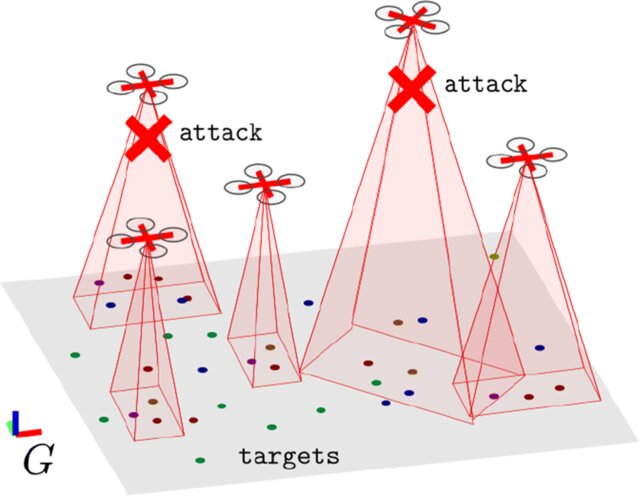
\includegraphics[width=0.7\textwidth]{figures/swarm2.jpeg}
    \end{subfigure}
    \begin{subfigure}[b]{0.49\textwidth}
        \centering
        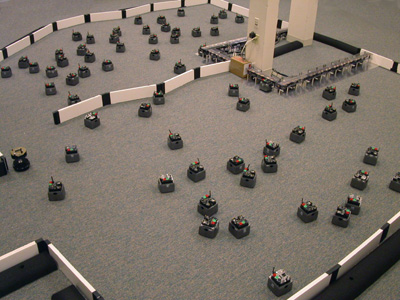
\includegraphics[width=0.6\textwidth]{figures/swarm3.jpeg}
    \end{subfigure}
    \begin{subfigure}[b]{0.49\textwidth}
        \centering
        
\includegraphics[width=0.7\textwidth]{figures/smartcity2.jpeg}
    \end{subfigure}
    \begin{subfigure}[b]{0.49\textwidth}
        \centering
        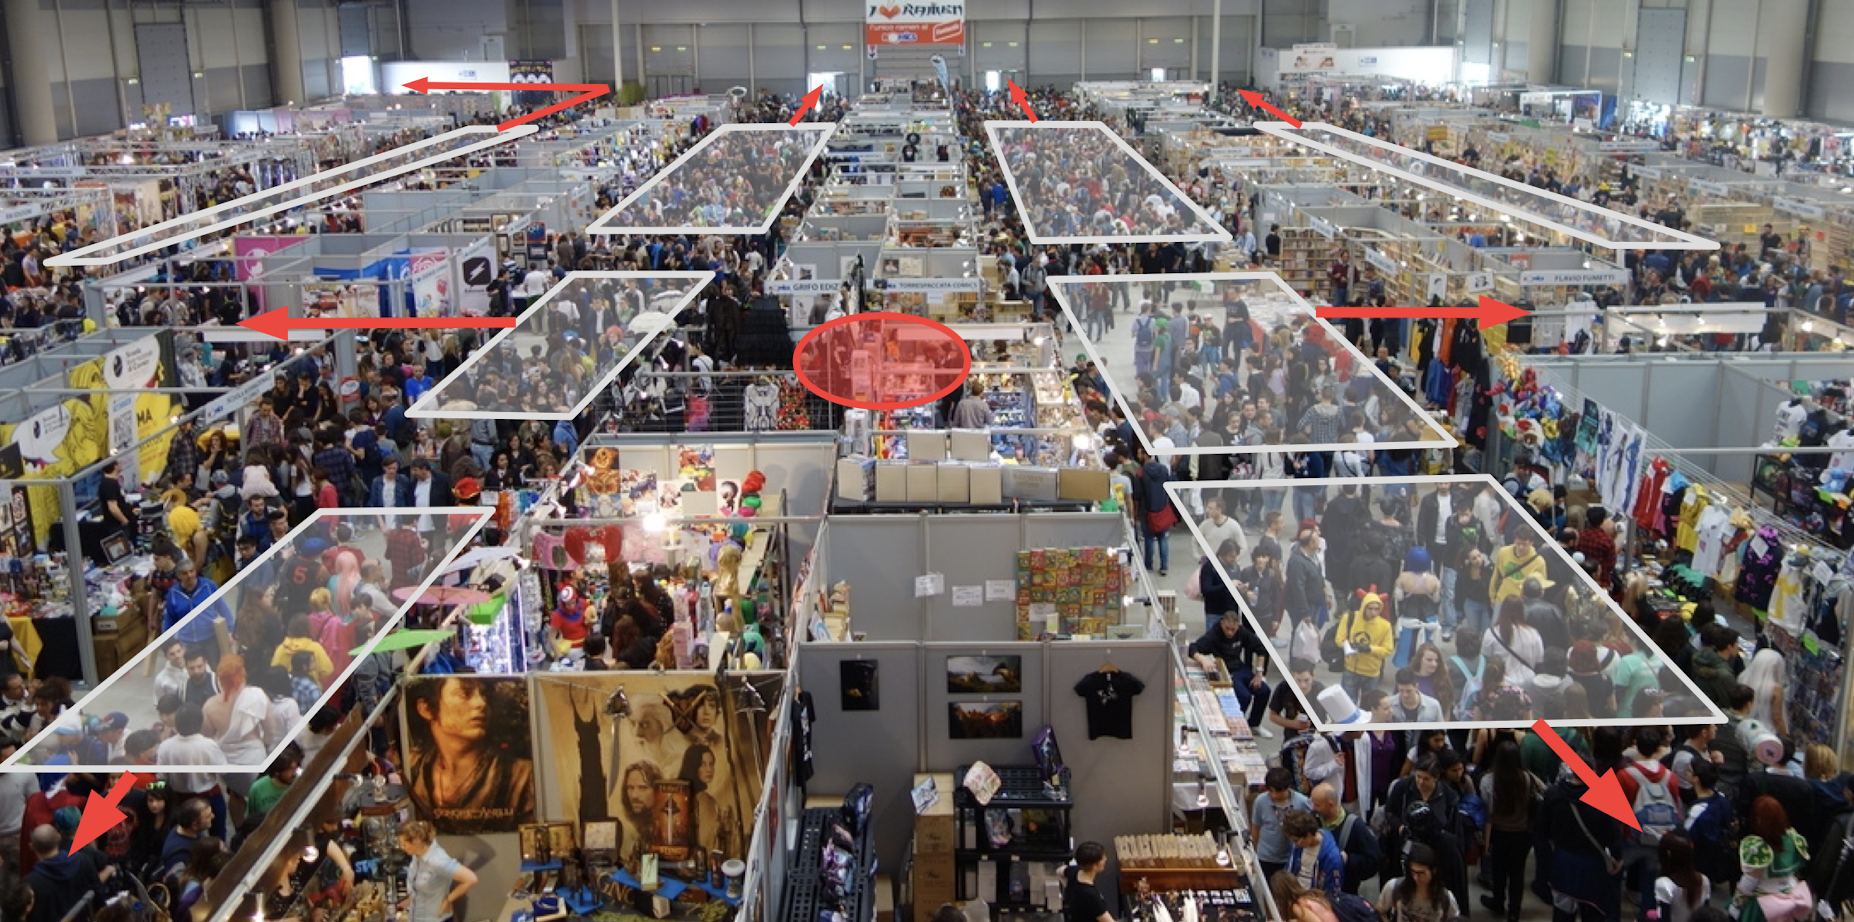
\includegraphics[width=0.7\textwidth]{figures/crowd.png}
    \end{subfigure}
    \caption{Some examples of Cyber-Physical Swarms.}%\vspace{-10pt}
    \label{fig:cpsw}
\end{figure*}


Swarms have been extensively studied due to a series of significant advantages, namely:
    i) \emph{cost}: the devices used are typically simpler than a single device that could solve the task individually, resulting in lower costs;
    ii) \emph{fault-tolerance}: simpler devices are less prone to failures, and there is no single point of failure;
    iii) \emph{scalability}: the system can be easily scaled by adding or removing devices;
    iv) \emph{robustness}: the system can handle the loss of some devices;
    v) \emph{flexibility}: the same system can solve different tasks.


%
\section{Aggregate Computing}

\paragraph{Context}
Over the last few years, there has been a definite trend in the development of computational devices: 
    they have been getting smaller, powerful, and less expensive. We have moved from using a 
    single mainframe computer that is shared by an entire department at a company or university, 
    to using numerous individual devices like smartphones, smartwatches, and others, all interconnected
    with one another. This phenomenon has led to a range of opportunities, but it has also introduced 
    new challenges when it comes to engineering these \emph{complex distributed systems}. It soon became clear 
    that conventional microprogramming approaches, which involve programming each device separately, lacked of 
    \emph{modularity} and \emph{reusability}. For this reason, attempts have been made to introduce novel paradigms, including 
    macroprogramming, which shifts focus onto the \emph{collective of devices}, considering their neighbourhood 
    relations and interactions.
    Some paradigms that have gained significant attention in recent years are \emph{aggregate computing (AC)} \cite{AC}, 
    \emph{tuple on the air (TOTA)} \cite{tota} and \emph{buzz} \cite{7498536}.

\paragraph{Field calculus}
\emph{Field calculus (FC)} \cite{fieldcalculus} has been designed to be a minimal core calculus aimed at capturing the essential 
    aspects of languages that make use of \emph{computational fields}, somewhat similarly to what $\lambda$-calculus does for 
    representing the essence functional programming. 
    The computational model of FC proposes that a program \textbf{P} is executed by a network of devices $\delta$, with a concept 
    of \emph{neighborhood relation} representing physical or logical proximity. An example of such a network is shown in \Cref{fig:random-network}. 
    This notion of neighborhood is used to represent devices capable of direct communication, such as sensors within a broadcast range. 
    In addition to this, the computational model also defines the concept of \emph{computational field} $\phi$. 
    These fields \cite{VIROLI2019100486, 1316820} are 
    a distributed data structure that maps each device, at a given time, to a value.

\begin{figure*}[t]
    \centering
    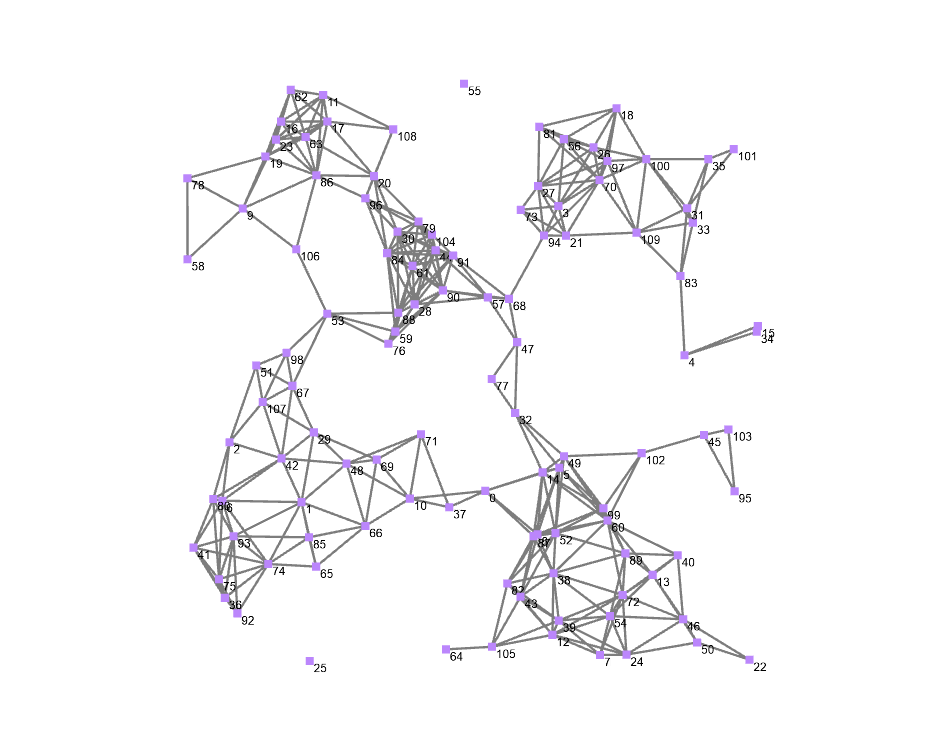
\includegraphics[width=0.7\textwidth]{figures/scafi-web-example.png}
    \caption{A random network of devices generated using ScaFi Web. 
        Each purple dot represents a device, and each line represents a neighbour relation.}
    \label{fig:random-network}
\end{figure*}

A key aspect of FC is that the program (or specification) \textbf{P} can be interpreted both 
    \emph{locally} and \emph{globally}. Locally, it is viewed as a description of computation on 
    an individual device, which is executed in asynchronous \emph{computational rounds}. 
    Each round consists of three phases:
    i) \emph{context building}, each device collects information from the 
         neighborhood and sensors and aggregates it to build its own local context,
    ii) \emph{program execution}, each device executes the aggregate program on the local context, and
    iii) \emph{export sharing}, each device shares the result of the computation with the neighborhood.
    When a device completes a round, it is said ``\emph{the device fires}".
    Globally, on the other hand, a given expression \textsf{e} specifies a mapping that associates, 
    for each round of each device, the value \textsf{e} assumes at that specific space-time event.
    This dualism inherently enables the alignment of each device's individual behaviour with the 
    emerging global behaviour of the entire network of devices.

\Cref{fig:fc-syntax} gives the basic \emph{abstract syntax} of field calculus. Following this syntax 
    a program P is defined as a sequence of function declarations $\bar{F}$ followed by the main 
    expression $e$. An expression can be: 
    \begin{itemize}
        \item A variable $x$ (e.g., a function parameter)
        \item A value $v$. It can be of two types:
        \begin{itemize}
            \item A \emph{local} value $l$ (e.g., a Boolean or an Integer);
            \item A \emph{neighbouring (field)} value $\phi$. It represents a collection of values 
                from neighbors that maps, for each device, the set of neighbour devices $\delta$
                (including the device itself) to local values $l$ (e.g., a map of neighbours to the distances 
                to those neighbours).
        \end{itemize}
        \item A function call $f(\bar{e})$ to either a user-declared function or a built-in function;
        \item A \emph{branching expression} that splits the system into two sub-region depending on 
            how each device evaluates the condition;
        \item The \texttt{nbr} construct, that defines a neighbouring value field $\phi$ that maps 
            each neighbor with its latest available result of evaluating $e$;
        \item The \texttt{rep} construct, which models state evolution over time.
    \end{itemize}

    \begin{figure*}[t]
        \centering
        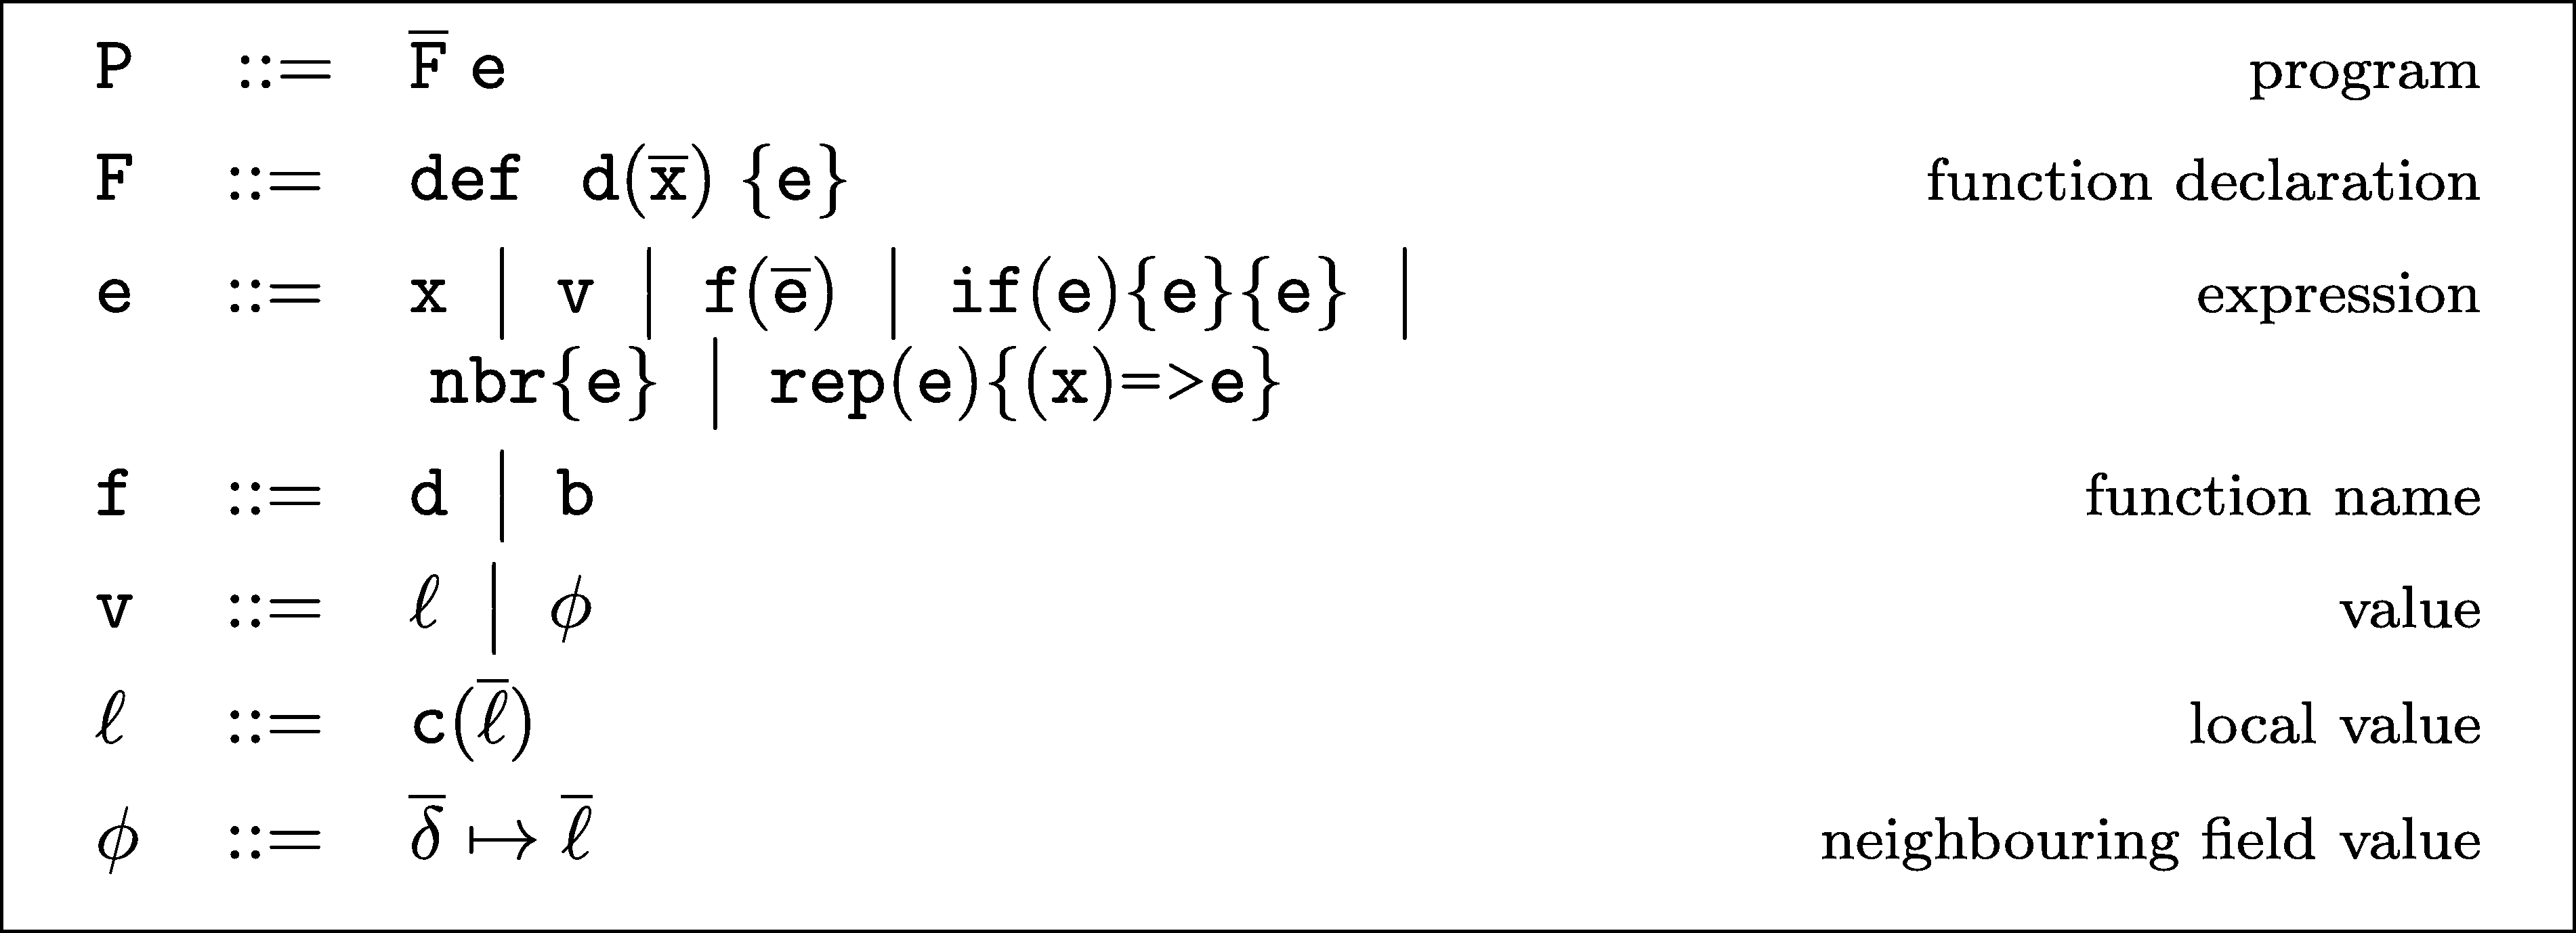
\includegraphics[width=0.8\textwidth]{figures/FC-abstract-syntax.png}
        \caption{Field calculus abstract syntax. From \cite{fieldcalculus}.}
        \label{fig:fc-syntax}
    \end{figure*}

In addition to the syntax explained for FC, there is an expanded version for \emph{higher-order FC}. 
    Here, functions are considered \emph{first-class values} and programmers are able to pass functions as parameters 
    to other functions. This allows for the addition or modification of existing code within the network.

One final important aspect of field calculus is its ability to formally demonstrate the 
    validity of significant properties, including:
    \begin{itemize}
        \item \emph{self-stabilisation} \cite{viroli2018engineering, dolev2000self,lafuente2015fixpoint}:
        this feature serves to prevent the system from entering incorrect states. Firstly, it guarantees that, given a costant input, a program's 
        execution will converge to a specific value in a finite time for each device. Secondly, it ensures that this value is solely 
        dependent on the input and not on previous execution history.
        \item \emph{global coherence}: this characteristic is assured by the field calculus, which ensures consistent alignment of the \emph{nbr}
        operator across the network. However, achieving this isn't straightforward, as multiple requests for \emph{nbr} can occur, 
        and the execution speed of functions can vary depending on the device. 
        If global-local coherence isn't maintained, there may come a point where a subset of network devices loses 
        synchronization with the entire network.
        \item \emph{space-time universality} \cite{audrito2018space}: this property guarantees that field calculus is computationally 
        universal (or Turing complete \cite{turing2009computing, turing1936computable}) and that it can be used to solve any computable problem.
        \item \emph{eventual consistency} \cite{beal2017self}
    \end{itemize}
    

\paragraph{Agregate computing}
\emph{Aggregate computing} \cite{AC} is a macro-programming model theoretically based on \emph{field calculus}, providing innovative solutions
    to the issues previously mentioned. Like FC, it puts the collective of devices (i.e., the \emph{aggregate system})  at its core 
    rather than individual devices. AC's objective is to reduce the complexity of designing, developing, 
    and maintaining complex distributed systems, with focus on three fundamental aspects:
    i) the composition of modules and subsystems must transparent,
    ii) different subsystems needs different coordination mechanisms for different regions and times, and 
    iii) the implementation details of coordination mechanisms should be hidden from programmers in order to facilitate ease of use.
    To attain this objective, AC adopts a \emph{layer-based architecture} (\Cref{fig:ac-layers}) that, in addition to field calculus, 
    includes two levels of abstraction to increase resilience and hide complexity. 


\begin{figure*}[t]
    \centering
    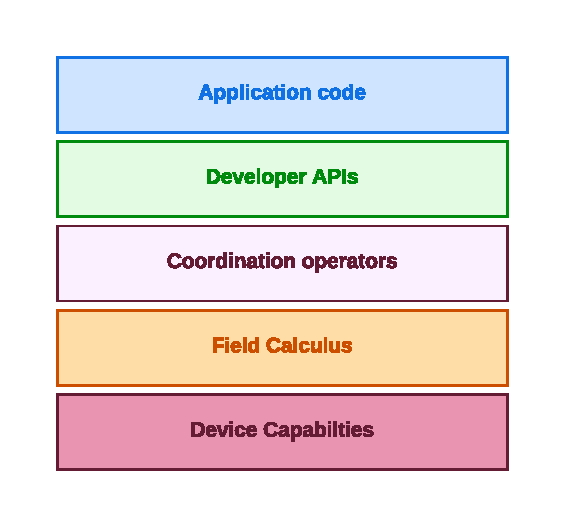
\includegraphics[width=0.7\textwidth]{figures/AC-layers.pdf}
    \caption{Aggregate programming abstraction layers.}
    \label{fig:ac-layers}
\end{figure*}

The first additional layer, placed immediately above the FC layer, is crucial for hiding complexity and supporting the 
    efficient engineering of distributed coordination systems. In practice, it introduces various operators that can 
    be used by the subsequent levels as building blocks, namely:
    i) \textbf{G} allows the spread of information from a source to a given distance,
    ii) \textbf{C} is the inverse of G, allowing the collection of information,
    iii) \textbf{T} allows to keep track of the time, and
    iv) \textbf{S} allows the election of a set of leaders and the partition of the network according to those leaders. 
The second-to-last layer comprises libraries and features tailored towards offering a simple interface for 
    software developers. Furthermore, this layer encourages reusability, productivity, declarativeness, 
    flexibility, and efficiency. An instance of a robust API is \emph{ScaFi} \cite{casadei2022scafi}, a Domain-Specific 
    Language for implementing aggregate computing via the Scala programming language.
Finally, there is the application layer, where the end-user can integrate their own services based on aggregate computing, 
    such as a crowd monitoring system in a smart city.

\paragraph{ScaFi}
\emph{ScaFi} \cite{casadei2022scafi} is a toolkit for the Scala language that provides a domain-specific language, libraries, 
    a simulation environment and runtime support for developing aggregate computing based systems.

\begin{figure*}[t]
    \centering
    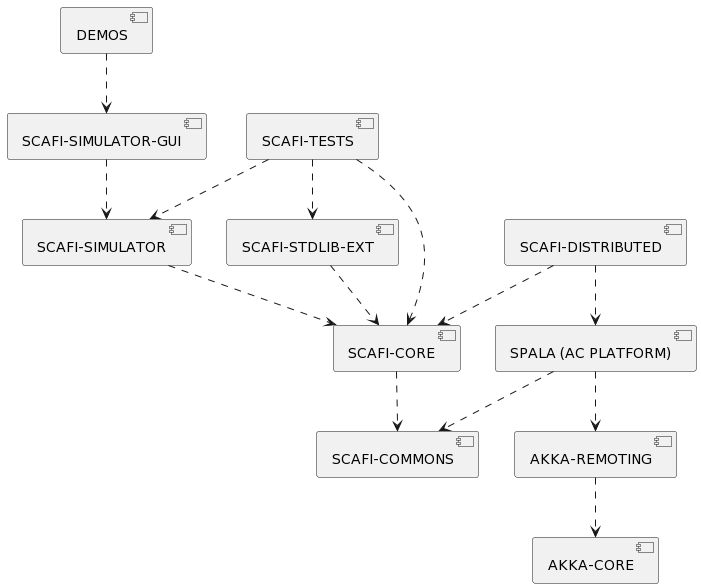
\includegraphics[width=0.8\textwidth]{figures/scafi-arc.png}
    \caption{ScaFi toolkit high level architecture.}
    \label{fig:scafi-arc}
\end{figure*}

The architecture of ScaFi consists of various modules (\Cref{fig:scafi-arc}), the main ones being:
    i) \texttt{scafi-core}, which contains the DSL and a standard library of reusable functions 
        (e.g., Gradients, BlockG and BlockS),
    ii) \texttt{scafi-stdlib-ext}, which provides a set of additional functions; as these require external dependencies, 
        it is kept separate from the core,
    iii)\texttt{scafi-simulator}, which offers support for simulating aggregate systems,
    iv) \texttt{scafi-simulator-gui}, which provides a GUI for visualizing and interacting with the simulation,
    v) \texttt{spala}, which provides an actor-based middleware for AC based on Akka \cite{hunt2014introduction},
    vi) \texttt{scala-distributed}, which provides an integration layer for spala in ScaFi.

An example of how ScaFi works is shown in \Cref{fig:channel} and \Cref{lst:channel}, the goal is create a channel given 
    a source, a destination and a width. To reach this goal is it possible to define the computation as a pure function 
    over fields that exploits and composes the following functions:
    i) \texttt{gradient}, which takes as input a field of Booleans and computes in output a field of Integers with the 
        mininum distance, for each point, from a given source represented by the values set to true in the input;
    ii) \texttt{distance}, which computes the distance between two sources, and
    iii) \texttt{dilate}, which takes as input a field of Booleans and stretches the source by a given width.

\begin{figure}[h!]
    \centering
    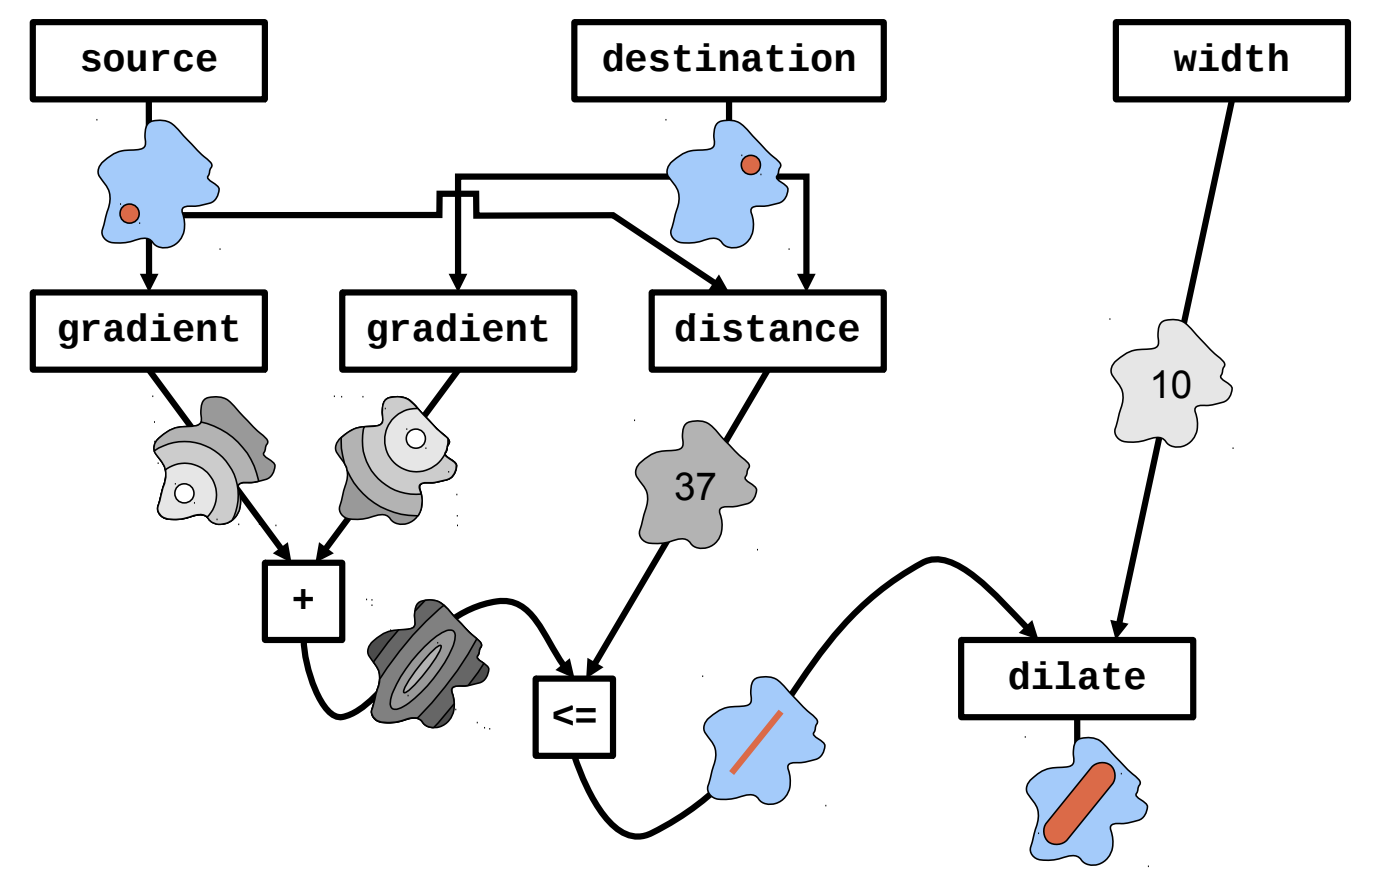
\includegraphics[width=0.7\textwidth]{figures/channel.png}
    \caption{A ScaFi AC program example. This algorithm representation is obtained from the code in \Cref{lst:channel}}.
    \label{fig:channel}
\end{figure}

\begin{lstlisting}[caption={A ScaFi AC program example. The algorithm implements a channel between a source and a destination.}, label={lst:channel}]
def channel(
    source: Boolean, 
    destination: Boolean, 
    width: Double
): Double {
    dilate(gradient(source) + gradient(destination) 
        <= distance(source, destination), width)
}
\end{lstlisting}

\begin{figure*}[h!]
    \centering
    \begin{subfigure}[b]{0.49\textwidth}
        \centering
        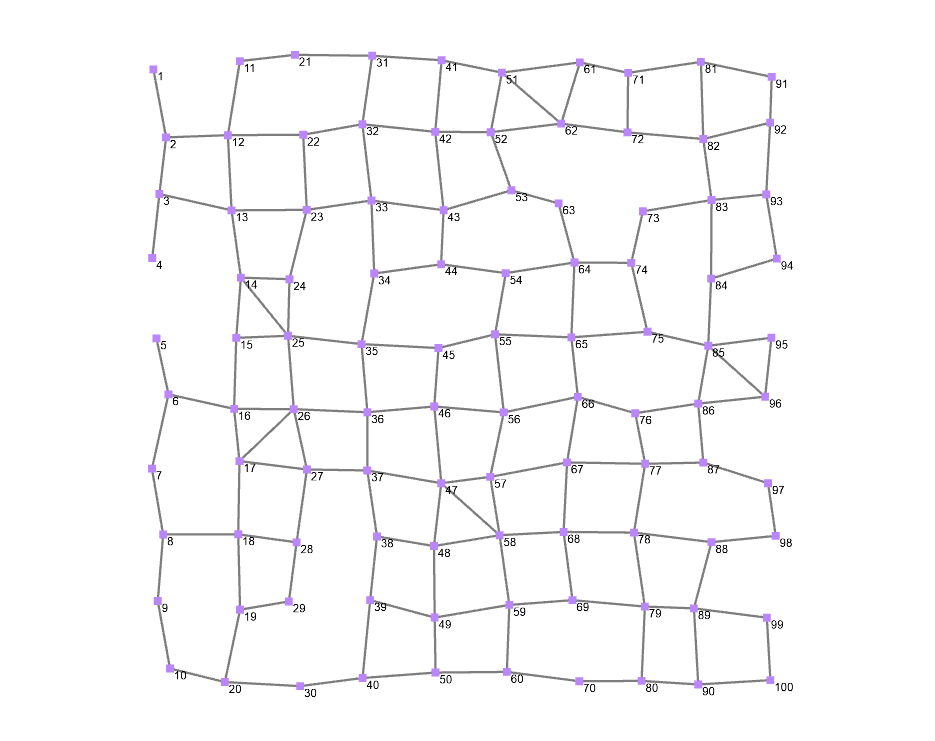
\includegraphics[width=\textwidth]{figures/channel1.png}
    \end{subfigure}
    \hfill
    \begin{subfigure}[b]{0.49\textwidth}
        \centering
        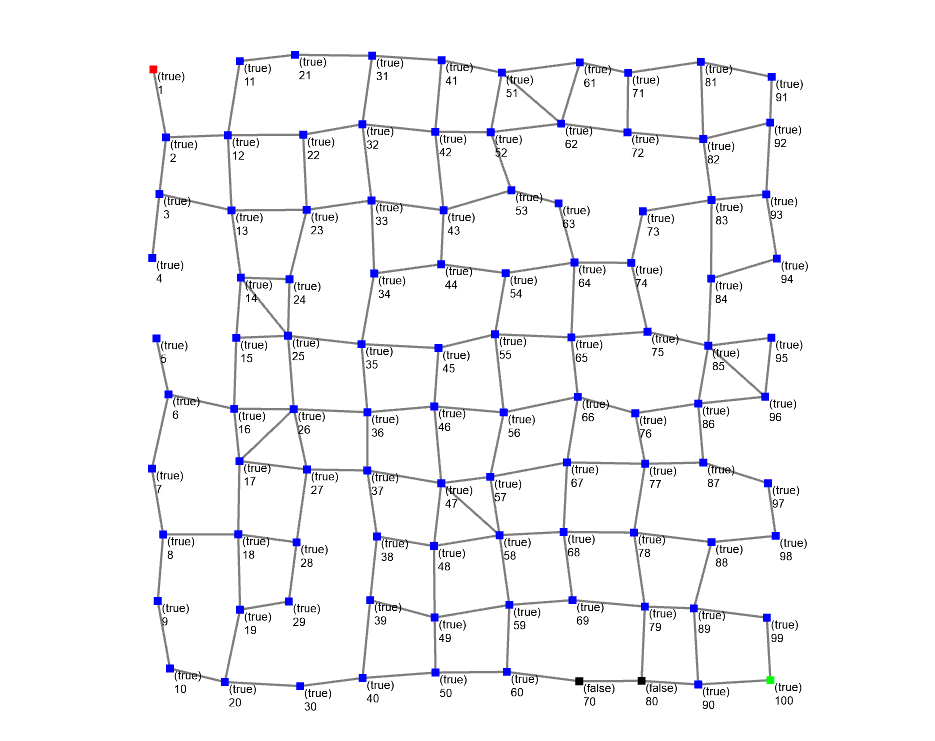
\includegraphics[width=\textwidth]{figures/channel2.png}
    \end{subfigure}
    \hfill
    \begin{subfigure}[b]{0.49\textwidth}
        \centering
        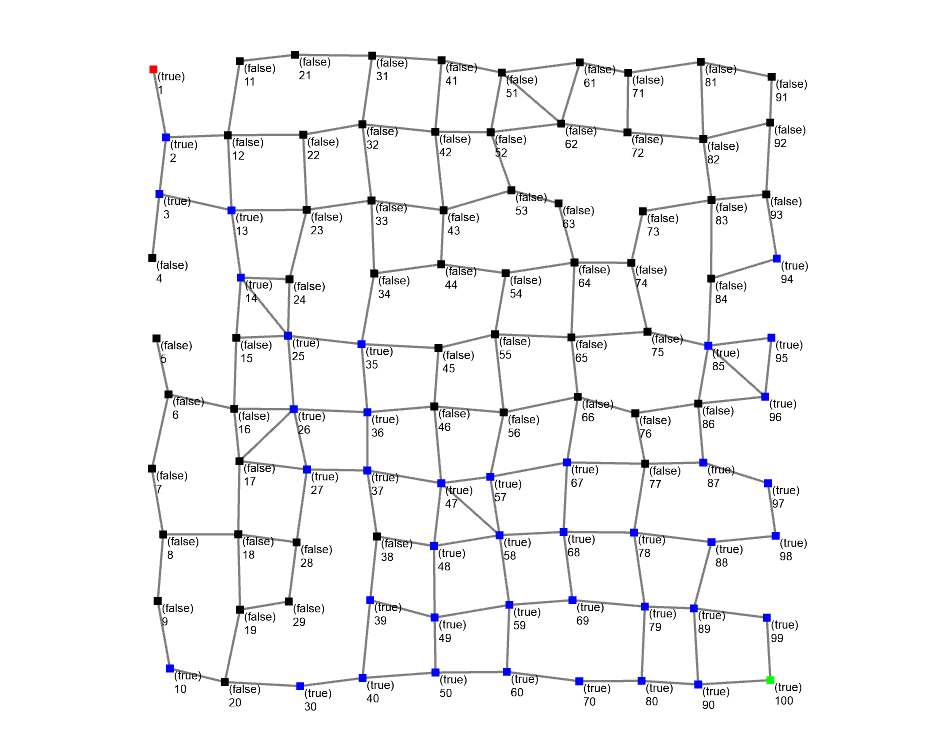
\includegraphics[width=\textwidth]{figures/channel3.png}
    \end{subfigure}
    \hfill
    \begin{subfigure}[b]{0.49\textwidth}
        \centering
        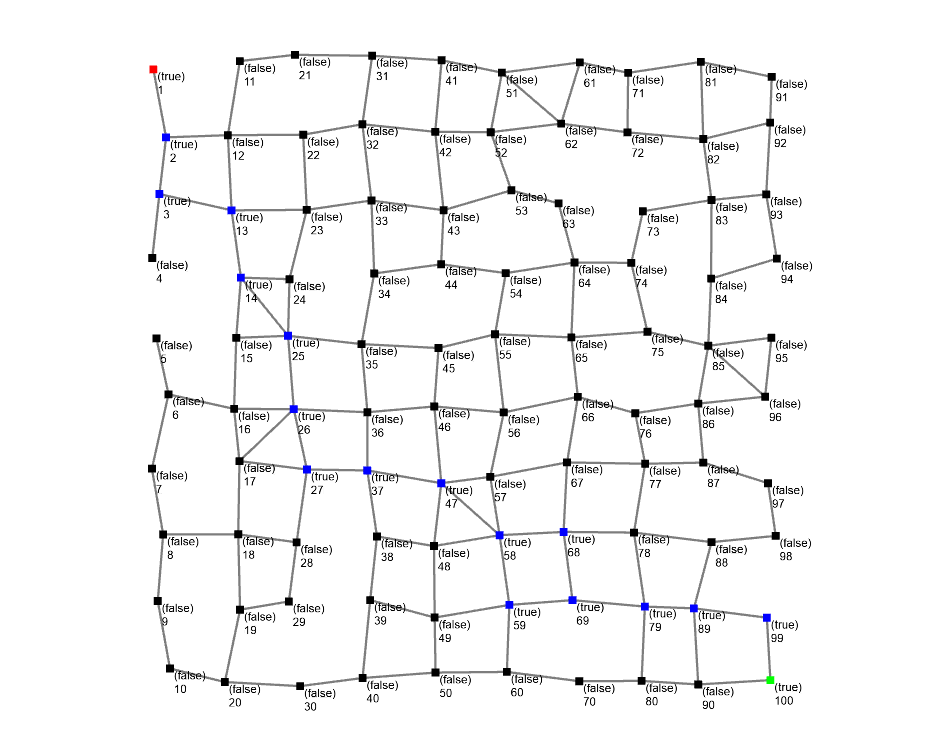
\includegraphics[width=\textwidth]{figures/channel4.png}
    \end{subfigure}
\caption{Channel algorithm execution on ScafiWeb. The source is the red dot, the destination is the green dot, 
    the time flows from left to right and from top to bottom.}
\label{fig:channel-scafiweb}
\end{figure*}


%
\section{Reinforcement Learning}
%

``\emph{Reinforcement Learning (RL)} is the science of decision making. It is about learning the optimal behavior 
    in a environment to obtain maximum reward" 
    \footnote{\url{https://www.synopsys.com/ai/what-is-reinforcement-learning.html}}.
    RL is a general framework, other than supervised and unsupervised learning, in which an \emph{agent} learns 
    to behave within an \emph{environment} by performing some \emph{actions} and seeing the result they produce.
    It is inspired by how humans and animals learn through the system of rewards and punishments: for each good action
    the environment provides to the agent a positive reward, instead, for each bad action the agent gets a negative 
    reward (also called penalty).

Formally, a RL problem can be formulated as following \cite{RLSurvey}:
    \begin{itemize}
        \item Discrete time steps $t=0, 1, 2, ...$;
        \item A discrete set of environment states $\mathcal{S}$;
        \item A discrete set of agent actions $\mathcal{A}$;
        \item A reward signal;
        \item A probabilistic policy $\pi$, that is a mapping function from states to actions.
    \end{itemize}
    The goal of the agent is to learn the optimal policy $\pi^*$ in order to maximize 
        some long-run measure of reinforcement (e.g., the Infinite Horizon Discounted Model \cite{RLSurvey}).
        First, at time $t$, the agent observes the state of the environment $s_t \in \mathcal{S}$
        and chooses an action $a_t \in \mathcal{A}$ using the actual policy $\pi_t$. 
        Thereafter, the environment: takes in the action $a_t$, emits the new state $s_{t+1} \in \mathcal{S}$ 
        and returns the scalar reward $r_{t+1}$ (\Cref{fig:rl_schema}).
        Finally, the agent, based on the reward obtained updates its knwoledge.
    This formulation stems from \emph{Markov Decision Processes}, which is a mathematical framework for \emph{sequential decision making}. A very important property that these systems must adhere to is the \emph{Markov property}, which states ``\emph{the future is independent of the past given the present.}" In other words, it implies that the state transition function does not require the entire past trajectory but only the last state, namely: 
    $$p(s_{t+1} | s_t, a_t, ..., s_0, a_0) = p(s_{t+1} | s_t, a_t)$$
    It is important to note that the concept of state can always be extended to satisfy this property.


\begin{figure}[t]
    \centering
    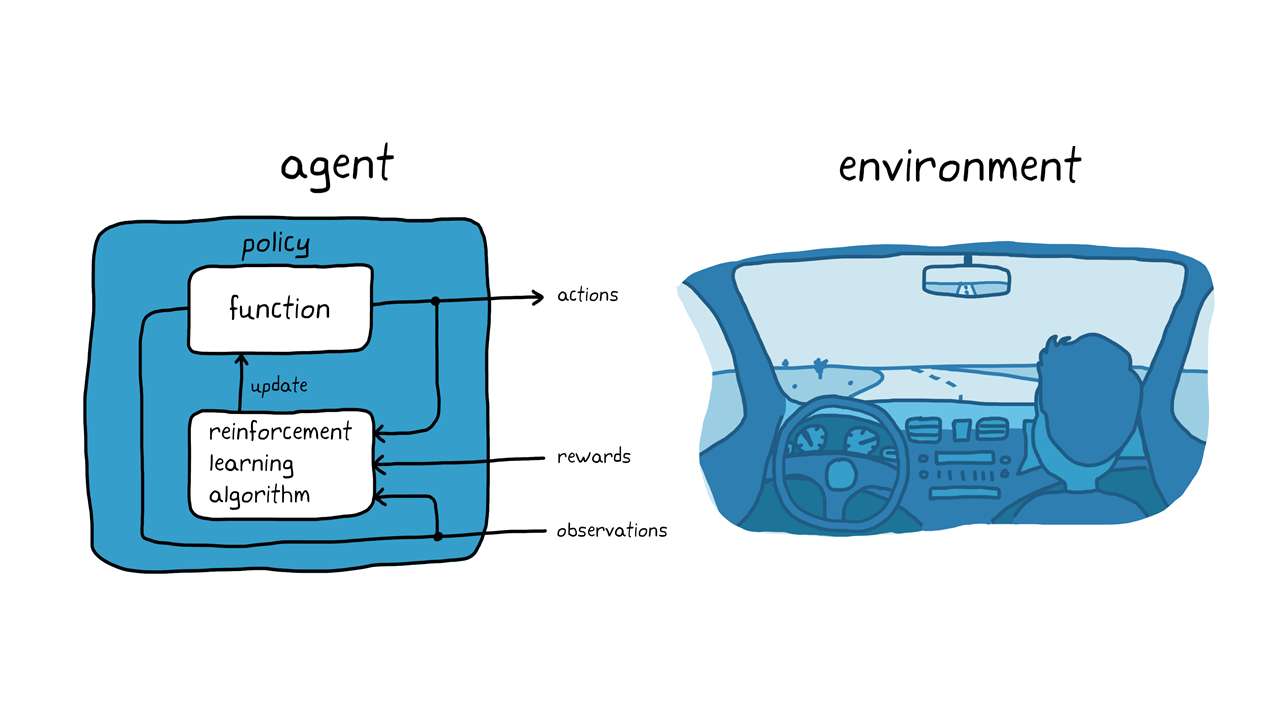
\includegraphics[width=0.7\textwidth]{figures/rl.png}
    \caption{Agent-environment interactions.}
    \fonte{\url{https://it.mathworks.com/discovery/reinforcement-learning.html}}
    \label{fig:rl_schema}
\end{figure}

In order to find the optimal policy $\pi^*$, the agent tries to maximize the expected cumulative reward.
    Since the environment is stochastic (i.e., the same action performed in the same state could lead to different 
    results over time) the more you look into the future the more the outcome could diverge.
    For this reason, it is common to use a model that takes less account of rewards that are far away in time 
    than those that are close in time:
    $$R_t = \sum_{i=t}^{\infty} \gamma^{i-t} \cdot R_{\pi(s_i)}(s_i, s_{i+1}) $$
    This model is called \emph{Infinite Horizon Discounted Model}, the key aspect is the hyper-parameter $\gamma$.
    It is a scalar weight in the range $[0;1]$, in this way, the further away the reward is in time, the smaller its weight.

\paragraph{Exploration-exploitation dilemma}

The \emph{exploration-exploitation dilemma} is a problem that comes from the definition of the RL process.
    In order to increase its knowledge and build an optimal policy, the agent needs to \emph{explore} the environment 
    in the hope of finding better actions. After some exploration, the agent might have found a set of 
    apparently rewarding actions, but, how can the agent be sure that the found actions are actually the best? 
    When should the agent continue to explore or else, when should it just \emph{exploit} its existing knwoledge?

Several exploration strategies have been proposed in the literature to solve this problem, the simplest is the
    \emph{$\epsilon$-greedy} strategy. The agent \emph{randomly explore} the environment with probability $\epsilon$
    while \emph{exploit} the current optimal action with probability $1-\epsilon$.

    $$
    \pi(s)=
    \begin{cases}
        \pi^*(s) & \text{with probability $1-\epsilon$} \\
        \text{\emph{random action}} & \text{with probability $\epsilon$}\\
    \end{cases} 
    $$ 

    Usually, at the beginning of the learning process $\epsilon$ starts near to $1$ (i.e., more exploration) and then decreases
    to $0$ as the agent learns more and more about the environment. 

\paragraph{Main approaches}

In Reinforcement Learning, there are two main families of approaches that can be used to categorize the 
    algorithms employed by an agent in finding the optimal policy. These are: 
    i) \emph{policy-based} methods, and 
    ii) \emph{value-based} methods.
    Policy-based algorithms aim to directly learn a function that maps each state to the best action to take 
    (or a probability distribution over a set of possible actions). On the other hand, value-based methods 
    seek to learn a function that maps each possible state to an expected value of being in that state. 
    This way, the agent can learn which states is more valuable and will take action that leads to it. 
    This comparison is well illustrated in \Cref{fig:rl-methods}.

An example of policy-based method is \emph{Proximal Policy Optimization (PPO)} \cite{ppo}, while an example of 
    value based-method is \emph{Q-Learning} \cite{QL}

\begin{figure*}[t]
    \begin{subfigure}[b]{0.49\textwidth}
        \centering
        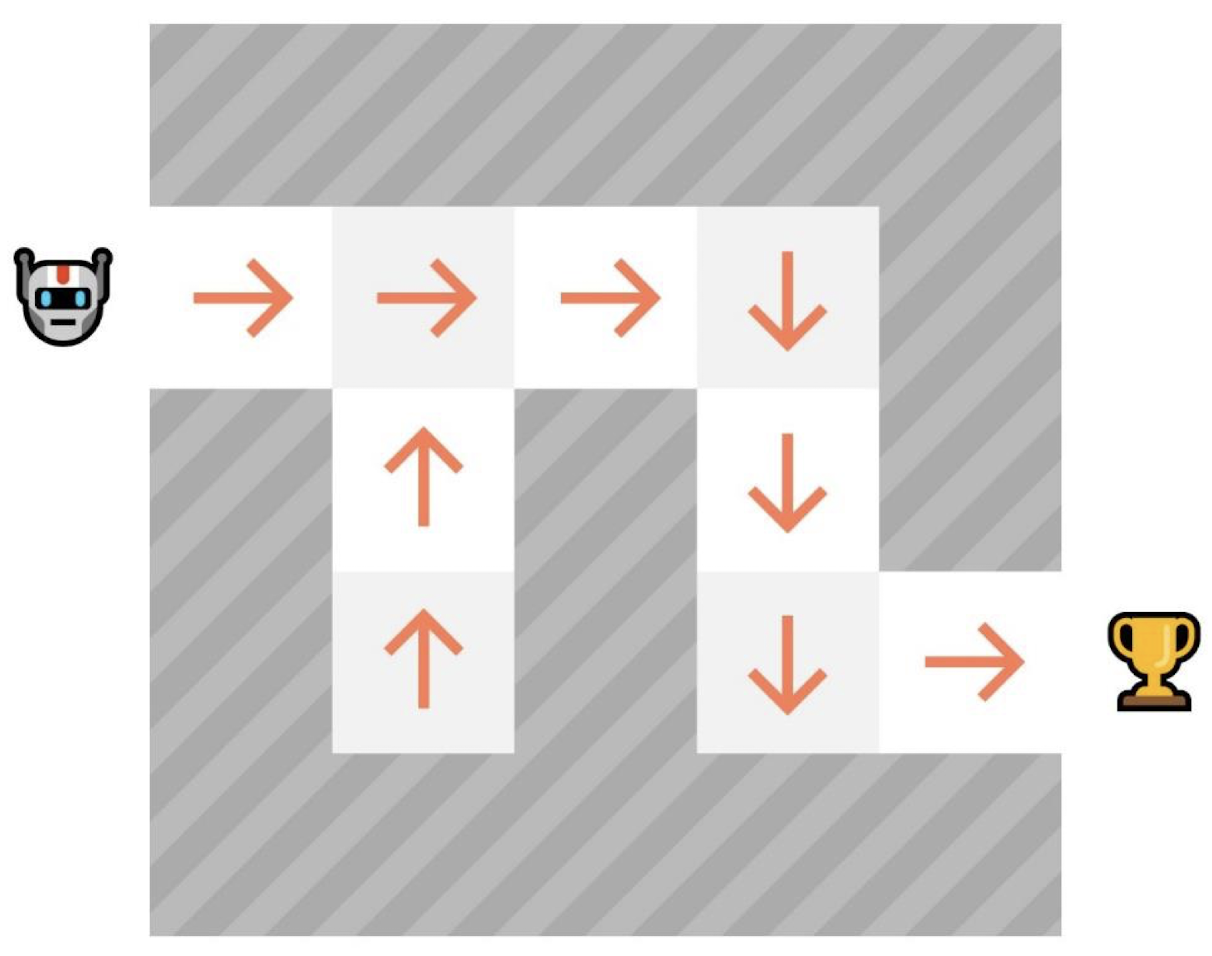
\includegraphics[width=0.7\textwidth]{figures/policy-based-rl.png}
        \caption{Policy based RL}
        \label{fig:policy-based-rl}
    \end{subfigure}
    \begin{subfigure}[b]{0.49\textwidth}
        \centering
        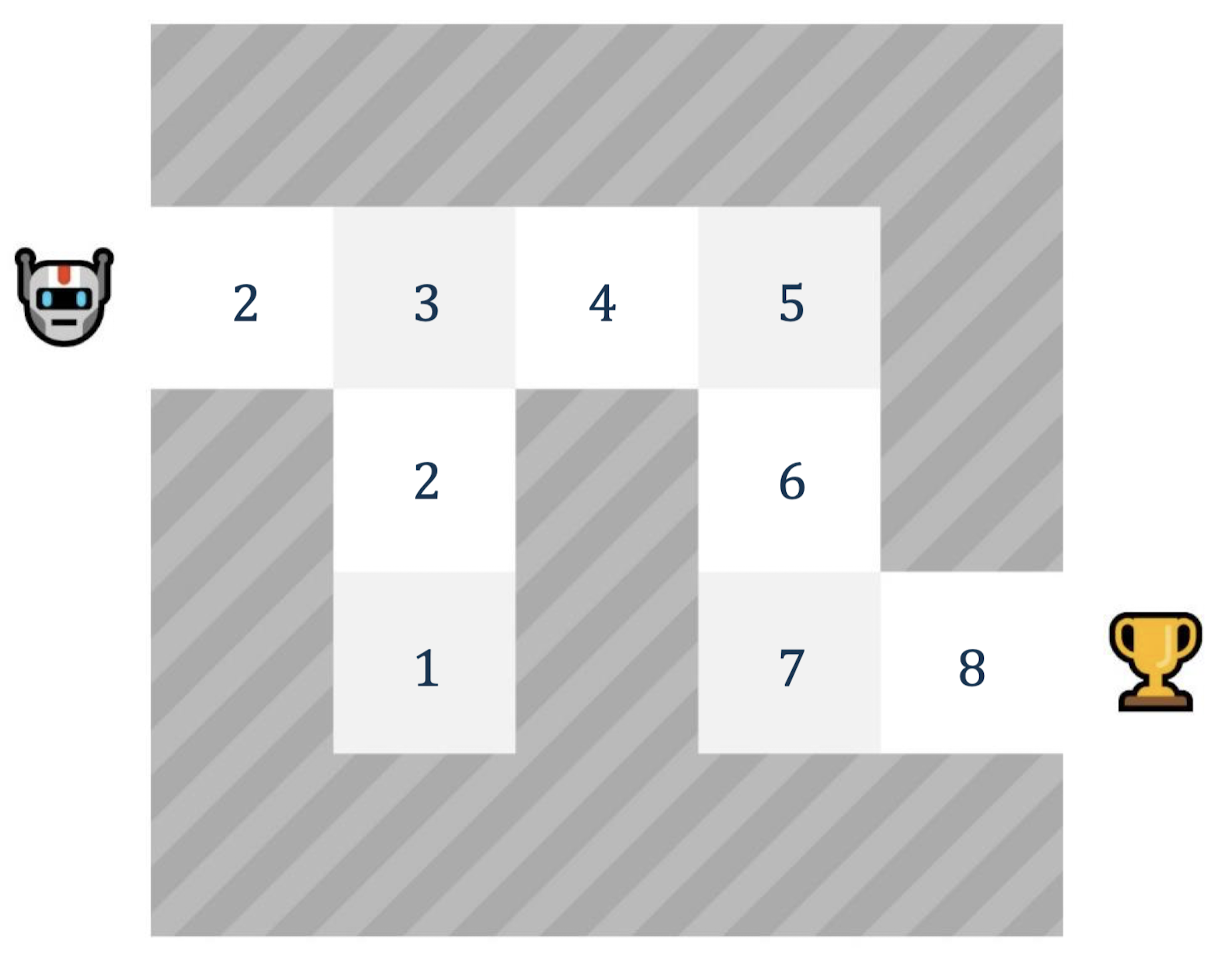
\includegraphics[width=0.7\textwidth]{figures/value-based-rl.png}
        \caption{Value based RL}
        \label{fig:value-based-rl}
    \end{subfigure}
\caption{Policy and value based algorithms visual comparison.}%\vspace{-10pt}
\fonte{\url{https://www.lamsalashish.com.np/blog/reinforcement-learning}}
\label{fig:rl-methods}
\end{figure*}

\paragraph{Q-Learning}

\emph{Q-Learning} is one of the most famous Reinforcement Learning algorithm from the value-based methods family. 
    One of the key aspects of this algorithm is the \emph{Q-Table}, denoted as $Q(s,a)$. This table represents, 
    for each possible state-action pair, the \emph{expected cumulative reward} that the agent will obtain by
    taking action $a$ in state $s$ and subsequently following optimal actions. 
    Thus, the Q-table at time step $t$, given a state $s_t$, an action $a_t$, and a policy $\pi_t$, is represented by:
    $$ Q(s_t, a_t) = max_{\pi(s_t) = a_t} R_{t+1}$$
    Starting from the Q-Table, it is possible to define the \emph{optimal policy} as follows:
    $$ \pi^{*}(s) = argmax_a Q^{*}(s,a) $$

Another key aspect is how we can estimate the reward at the end of the process if we only know the current state 
    and action, without knowing the subsequent trajectory. To achieve this, the \emph{Bellman equation} can be used. 
    This equation defines, for a given transition $<s_t, a_t, s_{t+1}, r_{t+1}>$, the value $Q(s,a)$ recursively 
    as the sum of the immediate reward and the maximum expected cumulative reward from the subsequent state:
    $$ Q(s_t,a_t) =  r_{t+1} + \gamma \cdot max_a Q(s_{t+1}, a)$$

The main idea of Q-Learning is to \emph{iteratively approximate} the Q-values, using the Bellman equation, as follows:
\[
Q(s_t,a_t) = 
    \underbrace{
        (1-\alpha) 
    }_\text{Learning Rate}   
    \cdot 
    \underbrace{
        Q(s_t,a_t) 
    }_\text{Old Value}
    + 
    \underbrace{
        \alpha
    }_\text{Learning Rate}
    \cdot 
    \overbrace{
        (
        \underbrace{
            r_{t+1}
        }_\text{Reward}
        + 
        \underbrace{
            \gamma
        }_\text{Discount Factor}
        \cdot 
        \underbrace{
        max_a Q(s_{t+1}, a)
        }_\text{Maximum Future Reward}
        )
    }^\text{Learned Value}
\]
    Where $\alpha$ is the learning rate hyper-parameter that controls how much of the current Q-value and newly proposed
    Q-value is considered.
    At the beginning of the learning process, these Q-values will be practically random estimates and may be completely wrong. 
    However, it has been demonstrated that as iterations progress, these Q-values will 
    converge and represent the true Q-values.

\paragraph{Deep Reinforcement Learning}

Classical algorithms of reinforcement learning, when applied in \emph{real-world contexts}, suffer from the problem of \emph{state space explosion}.
    This arises from an exceedingly large number of possible states, making the resolution of a given task \emph{computationally intractable}. 
    For instance, in the game of chess, there can be around $100^{100k}$ possible games, a number much larger than 
    the count of sand grains on Earth ($\approx 10^{23}$) and the number of atoms in the observable universe 
    ($\approx 10^{81}$). 
    For this reason, \emph{deep reinforcement learning} has been introduced, which involves utilizing deep neural networks
    as approximators for the policy and/or the value function.

One of the most well-known Deep RL algorithms is DQN \cite{dqn}. This was developed by DeepMind in 2013 and was initially
    used to train an agent capable of playing Atari video games. One of the advantages of using neural networks as 
    approximators for the function to be learned is the ability to avoid hand-engineering the state space and instead 
    allow the network to learn the best features directly. For example, in the case of Atari games, this is achieved 
    by using convolutional layers and feeding the network with screen raw pixels.
    
DQN, specifically, is the deep version of the Q-Learning algorithm, thus producing a Q-Value output for each 
    possible action (\Cref{fig:qlvsdqn}). This makes the training of the utilized neural network a regression task 
    in which a squared error loss can be employed as the loss function:
    $$ L = (y_t - \hat{y_t})^2 $$
    Where $y_t$ represents the actual value and $\hat{y_t}$ is the predicted value at time t. Since RL is an 
    unsupervised learning, and therefore labels are not available, the value $y_t$ is estimated using the 
    Bellman equation, transforming the loss function for a transition $<s_t, a_t, s_{t+1}, r_{t+1}>$ into:
    $$ L = ( r_{t+1} + \gamma \cdot max_a Q(s_{t+1}, a) - Q(s_t, a_t))^2 $$

\begin{figure*}[t]
    \begin{subfigure}[b]{0.49\textwidth}
        \centering
        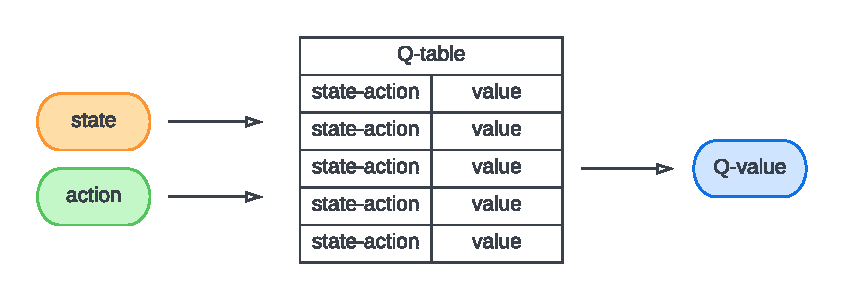
\includegraphics[width=\textwidth]{figures/q-learning.pdf}
        \caption{Q-Learning}
        \label{fig:ql}
    \end{subfigure}
    \begin{subfigure}[b]{0.49\textwidth}
        \centering
        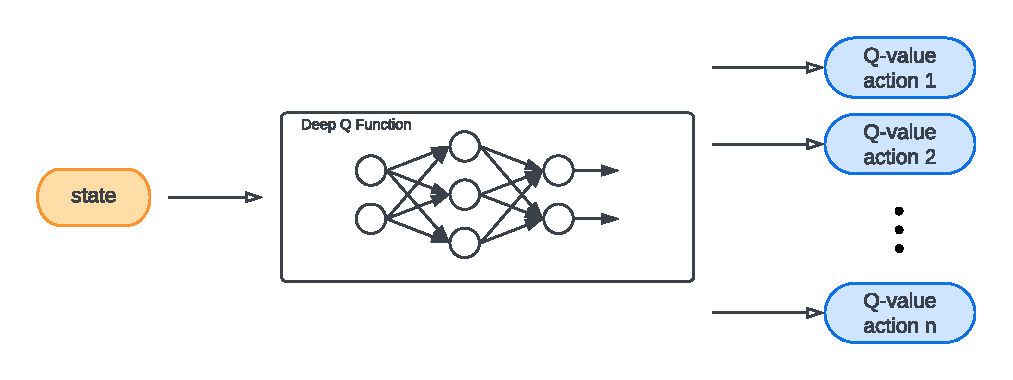
\includegraphics[width=\textwidth]{figures/deepQL.pdf}
        \caption{Deep Q-Learning}
        \label{fig:dqn}
    \end{subfigure}
\caption{Q-Learning and Deep Q-Learning visual comparison}\vspace{-10pt}
\label{fig:qlvsdqn}
\end{figure*}

When attempting to use neural networks to approximate the Q-function, several problems arise. 
    The first one is due to the high correlation that exists between two consecutive transitions within the same 
    episode. This correlation leads to a significant decrease in variance, causing the network to tend to forget 
    previous transitions as it overwrites them with newer ones. For instance, let's consider an agent's task to 
    learn to play a level-based video game; this issue implies that while the agent tries to learn how to navigate 
    the second level, it might forget how to behave in the first level. The most common solution is to employ an 
    \emph{experience replay} (i.e., a buffer), where all transitions $<s_t, a_t, s_{t+1}, r_{t+1}>$ are stored. 
    When updating weights, a random mini-batch is sampled from this buffer, breaking the correlation between consecutive
    transitions. Furthermore, since a transition can be used in multiple weight updates, this approach also 
    improves data efficiency.

A second issue that can be observed is referred to as the \emph{moving target problem}. This stems from the fact that,
    when updating the network's weights, both the predicted values and the target values are estimated using the 
    same neural network. This leads to a strong correlation between the target values and the network's weights, 
    introducing significant oscillations during training. To address this problem, two distinct neural networks 
    with identical architecture are employed: 
    i) \emph{the action network $Q$}, used to determine the agent's actions, which is updated every $u$ steps; 
    ii) \emph{the target network $\hat{Q}$}, used to calculate the target values, updated every $c$ steps. 
    Typically, $c >> u$, and the \emph{target network's} weight update involves replacing the existing weights with 
    those from the \emph{action network}.
    Since the target values are generated using an older set of weights, a delay is introduced between the 
    moment the $Q$ network is updated and the moment it starts to affects the target values.
    This delay reduces the likelihood of divergence and oscillations. The loss function becomes:
    $$ L = ( r_{t+1} + \gamma \cdot max_a \hat{Q}(s_{t+1}, a) - Q(s_t, a_t))^2 $$

\section{Multi-Agent Reinforcement Learning}
\emph{Multi-Agent Reinforcement Learning} is an extension of RL where multiple agents interact one another and 
    with the environment. 
    Usually, MARL is modelled as a \emph{Markov Game} (or Stochastic Game $\mathcal{S}$)~\cite{LITTMAN1994157} in
    which we have:
    \begin{itemize}
        \item A tuple $\mathcal{S} = <N, S, \{A^i\}, P, \{R^i\}>$ with $i \in 1 \dots N$
        \item The number of agents $N > 1$
        \item The action space of the i-th agent $A^i$. The global action space is defined as $\mathbb{A} = A^1 \times A^2 \times \dots \times A^N$
        \item A function describing the transition dynamics $P: S \times \mathbb{A} \rightarrow \mathcal{P}(S)$
        \item The reward function $R^i: S \times \mathbb{A} \times S \rightarrow \mathbb{R}$ for each agent $i$ 
    \end{itemize}

\paragraph{Categorization}

Based on the reward function used by the agents, MARL can be divided into three categories (\Cref{fig:marl-tasks}): 
    i) \emph{cooperative}, where all the agents trying to maximize the same reward function (e.g., a group of robots
    trying to clean a room); 
    ii) \emph{competitive}, where, potentially, each agent has its own reward function that is conflictual with the other (e.g., a rock-paper-scissor game). 
    iii) \emph{mixed}, where some agents are cooperative and others are competitive (e.g., a soccer game).
    Cooperative MARL, with respect to the policy, can be further divided into two additional categories, namely: 
    i) \emph{homogeneous}, where all the agents have the same capabilities, i.e., they use the same policy 
    ii) \emph{heterogeneous}, where each agent may have its own policy, in this case, each agent tries to maximize the local policy following the global shared goal.

\begin{figure*}[t]
    \centering
    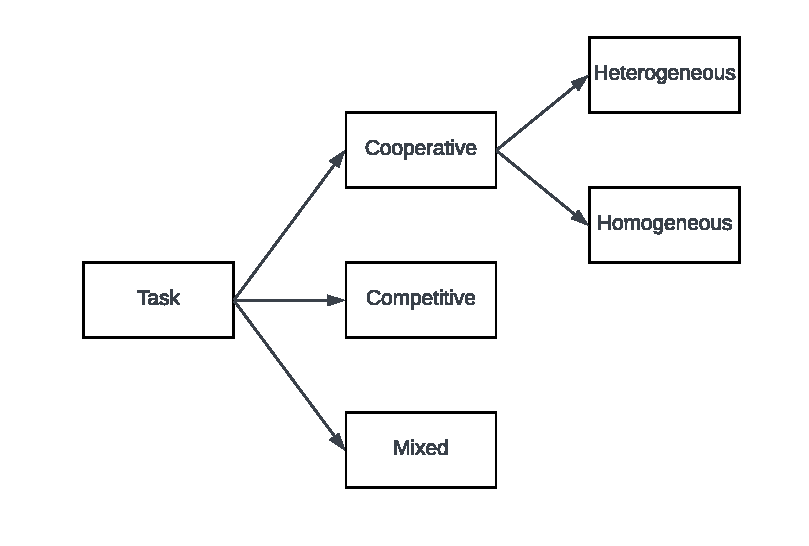
\includegraphics[width=0.8\textwidth]{figures/MARL-tasks.pdf}
    \caption{MARL tasks.}
    \label{fig:marl-tasks}
\end{figure*}

In this thesis, we focus on a subset of MARL, namely: \emph{Many Agent Reinforcement Learning}~\cite{yang2021many}. The only
    difference between the two approaches is in the number of agents involved. 
    Typically, in Many Agent Reinforcement Learning the number of agents may range from a hundred to one or two
    thousands whereas, in Multi Agent Reinforcement Learning, there are only a few tens~\cite{smac,marl-curricula}.
    Moreover, we focus on cooperative homogeneous and heterogeneous learning.


\paragraph{Training and execution model}
   
Another point to pay attention to is the system by which the training and execution of the various agents are carried out. This can be primarily categorized into three types (\Cref{fig:exmod}):
    i) \emph{Centralized Training Centralized Execution (CTCE)}, in this type of system, there is a higher-level agent called \emph{Learner}, with a global perspective, whose task is to perform training and compute actions to be undertaken. The remaining agents, therefore, transmit their local environmental perceptions (i.e., the local state) to the learner agent, which is responsible for merging these perceptions to reconstruct the global state. Once reconstructed, it selects the action to take in accordance with the current policy and evaluates the reward function for policy updates;
    ii) \emph{Centralized Training Decentralized Execution (CTDE)}, in this type of system, a learner agent with a global perspective executes the training algorithm. Once the policy is updated, it is sent to each agent, which can interact with the environment and take actions in accordance with it;
    iii) \emph{Decentralized Training Decentralized Execution (DTDE)}, in this type of system, each agent has its own local policy and can only observe a portion of the environment. Each agent, therefore, takes actions based on its perception of the environment and updates its own local reward function accordingly.

\begin{figure*}[t]
    \begin{subfigure}[b]{0.32\textwidth}
        \centering
        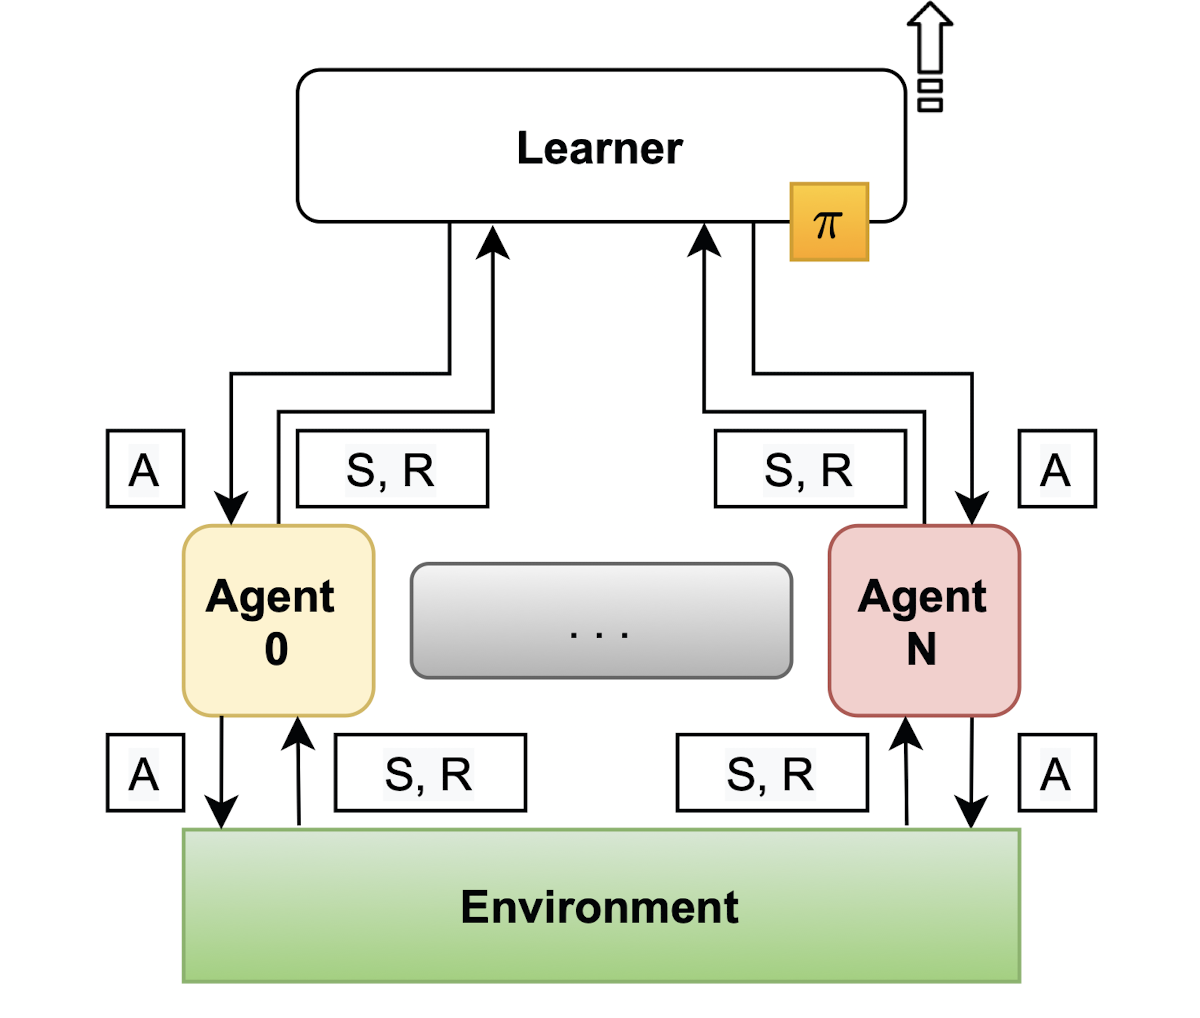
\includegraphics[width=\textwidth]{figures/CTCE.png}
        \caption{CTCE}
        \label{fig:ctce}
    \end{subfigure}
    \begin{subfigure}[b]{0.32\textwidth}
        \centering
        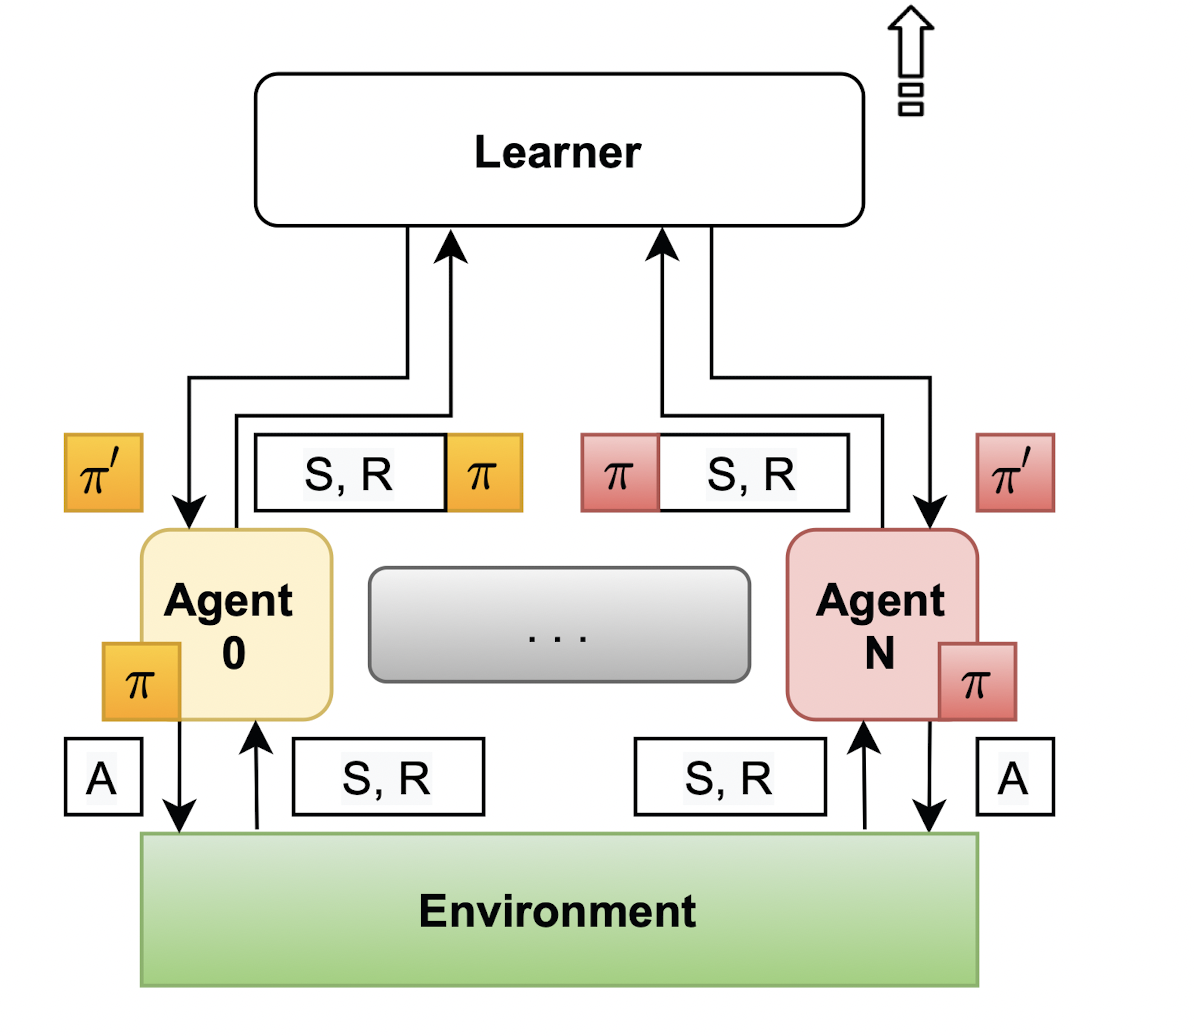
\includegraphics[width=\textwidth]{figures/CTDE.png}
        \caption{CTDE}
        \label{fig:ctde}
    \end{subfigure}
    \begin{subfigure}[b]{0.32\textwidth}
        \centering
        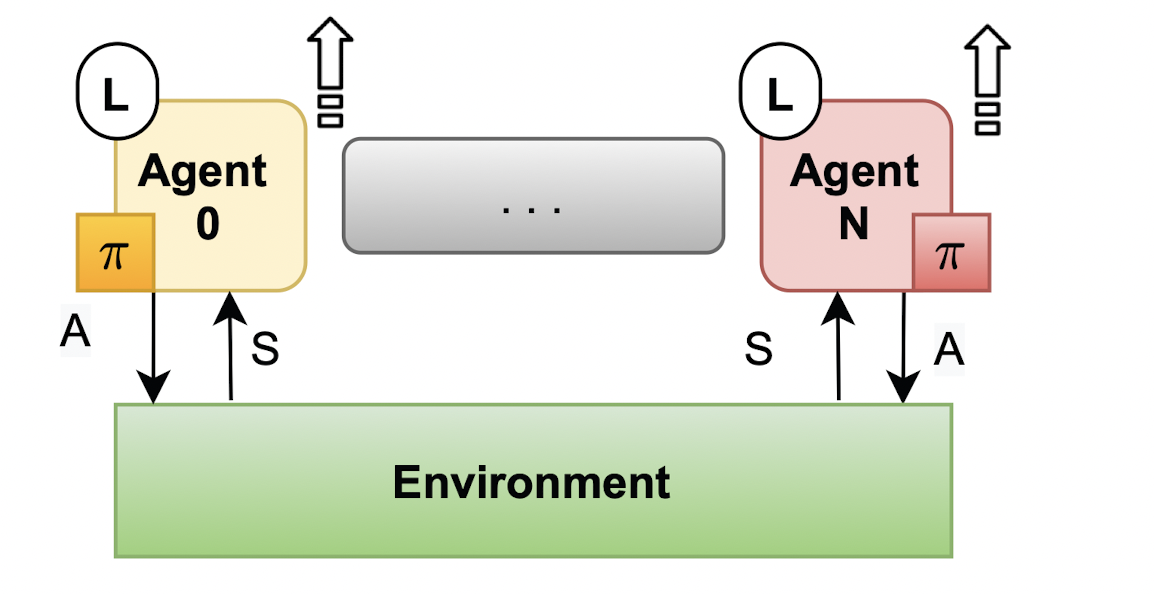
\includegraphics[width=\textwidth]{figures/DTDE.png}
        \caption{DTDE}
        \label{fig:dtde}
    \end{subfigure}
    \caption{MARL execution model comparison.}\vspace{-10pt}
    \label{fig:exmod}
\end{figure*}

\paragraph{Challenges}

MARL is a highly promising field that has been garnering increasing attention in recent years. Nevertheless, there are still several challenges that complicate its application in complex contexts. Some of these challenges include:
\begin{enumerate}
   

    \item  \emph{Partially Observable Environments}: in environments of significant complexity, agents cannot have a complete representation of the surrounding environment nor access the state of other present agents.
   
    \item \emph{Non-Stationarity}: this issue arises due to multiple agents simultaneously learning and changing the environment. From the perspective of an individual agent, the environment becomes non-stationary.
   
    \item  \emph{Agent Communication}: communication among agents is a crucial feature in the literature. The problem not only addresses what an agent should communicate but also with whom and when.
   
    \item  \emph{Coordination}: coordination is essential in cooperative systems, as agents must reach a consensus on the actions to take. Failure to coordinate during learning can lead to suboptimal policies. Coordination can be achieved through communication or implicitly, with each agent constructing its own model of other agents' behavior to infer their next actions.
   
    \item  \emph{Credit Assignment Problem}: this refers to associating a reward with an action taken by a specific agent. This association is crucial for learning to understand the effectiveness of an action and maximizing the reward function over time.
   
    \item  \emph{Scalability}: the scalability of these systems is influenced by the challenges outlined in this section. Training a single agent is inherently challenging; as the number of agents in the system increases, the complexity grows exponentially. Additionally, scalability is determined by an agent's robustness in the face of changes in the behavior of other agents. Literature presents exploration techniques to enhance scalability, such as knowledge reuse, regularization, adversarial training, and others.
\end{enumerate}

\section{Simulation}

In science and engineering, the use of \emph{simulators} plays a key role. These simulators enable the experimentation 
    with complex and expensive systems (such as cyber-physical swarms), offering a virtual 
    environment in which to conduct tests, analyses, and in-depth studies rapidly, under controlled and 
    repeatable conditions (e.g., \cite{argun2021simulation, bagrodia1998parsec, choi2021use, cannon2009simulation}).
    In this project, the \emph{Alchemist} \cite{alchemist} simulator has been taken as a reference.

Alchemist is a \emph{meta-simulator} designed for simulating \emph{complex distributed systems} in a rich variety of scenarios 
    like swarm robotics \cite{Casadei2021}, large-scale sensor networks \cite{Aguzzi_2022},
    crowd simulation \cite{Beal2015}, path planning, and even morphogenesis of multi-cellular systems.

This simulator is ``meta" \emph{by design}, this stems from the fact that it is based on general abstractions that
    can be mapped to specific use cases (i.e., \emph{incarnations}). The meta-model is inspired by biochemistry
    and consists of a set of \emph{nodes} that exist in an \emph{environment} and are linked together by 
    \emph{relationship} rules.
    Each node contains a sequence of \emph{molecules} and \emph{reactions}. 
    A \emph{molecule} represents a variable, which acts as a container for data. 
    \emph{Reactions} instead are events that occur based on a set of \emph{conditions}, and are fired according 
    to a time distribution, producing an effect that is described as an action. 
    This abstraction allows the simulator to be flexible and adaptable to a variety of use cases and node
    numbers (it could support thousands of nodes), while maintaining a consistent underlying structure

Alchemist features four incarnations: biochemistry, sapere, protelis, and ScaFi, 
    each with a different way of modeling molecules and actions.
    In this project, the \emph{ScaFi} incarnation has been taken as a reference.
    It supports the ScaFi Scala DSL and has been used in distributed peer-to-peer chats and 
    situated problem-solving

Alchemist offers an straightforward method for defining simulations. The process
    requires a YAML file that includes essential parameters, such as the incarnation
    type, neighbor connection model, and node deployment. In Figure 2, we have
    provided an example YAML file that creates a simulation using the ScaFi incarnation (first row). It also defines the neighborhood relationship based on fixed
    distances (0.5 in this case), placing nodes in a fixed grid of size 10x10 starting
    at -(5,5) and ending at (5,5), with a node-to-node distance of 0.25. Finally, it
    loads the ScaFi program called ``program", which is evaluated at each node with
    a frequency of 1.

\begin{figure*}
    \centering
    \begin{subfigure}[b]{0.49\textwidth}
        \centering
        \begin{lstlisting}[language=yaml]
    incarnation: scafi
    network-model:
        type: ConnectWithinDistance
        parameters: [0.5]
    deployments:
        type: Grid
        parameters: [-5,-5,5,5,0.25,0.25]
        /*dynamics of the simulation*/
        programs: 
            - program:
            - time-distribution: 1
                type: Event
                actions: 
                - type: RunScafiProgram
                    parameters: [program]
            - program: send
    \end{lstlisting}
    \end{subfigure}
    \hfill
    \begin{subfigure}[b]{0.49\textwidth}
        \centering
        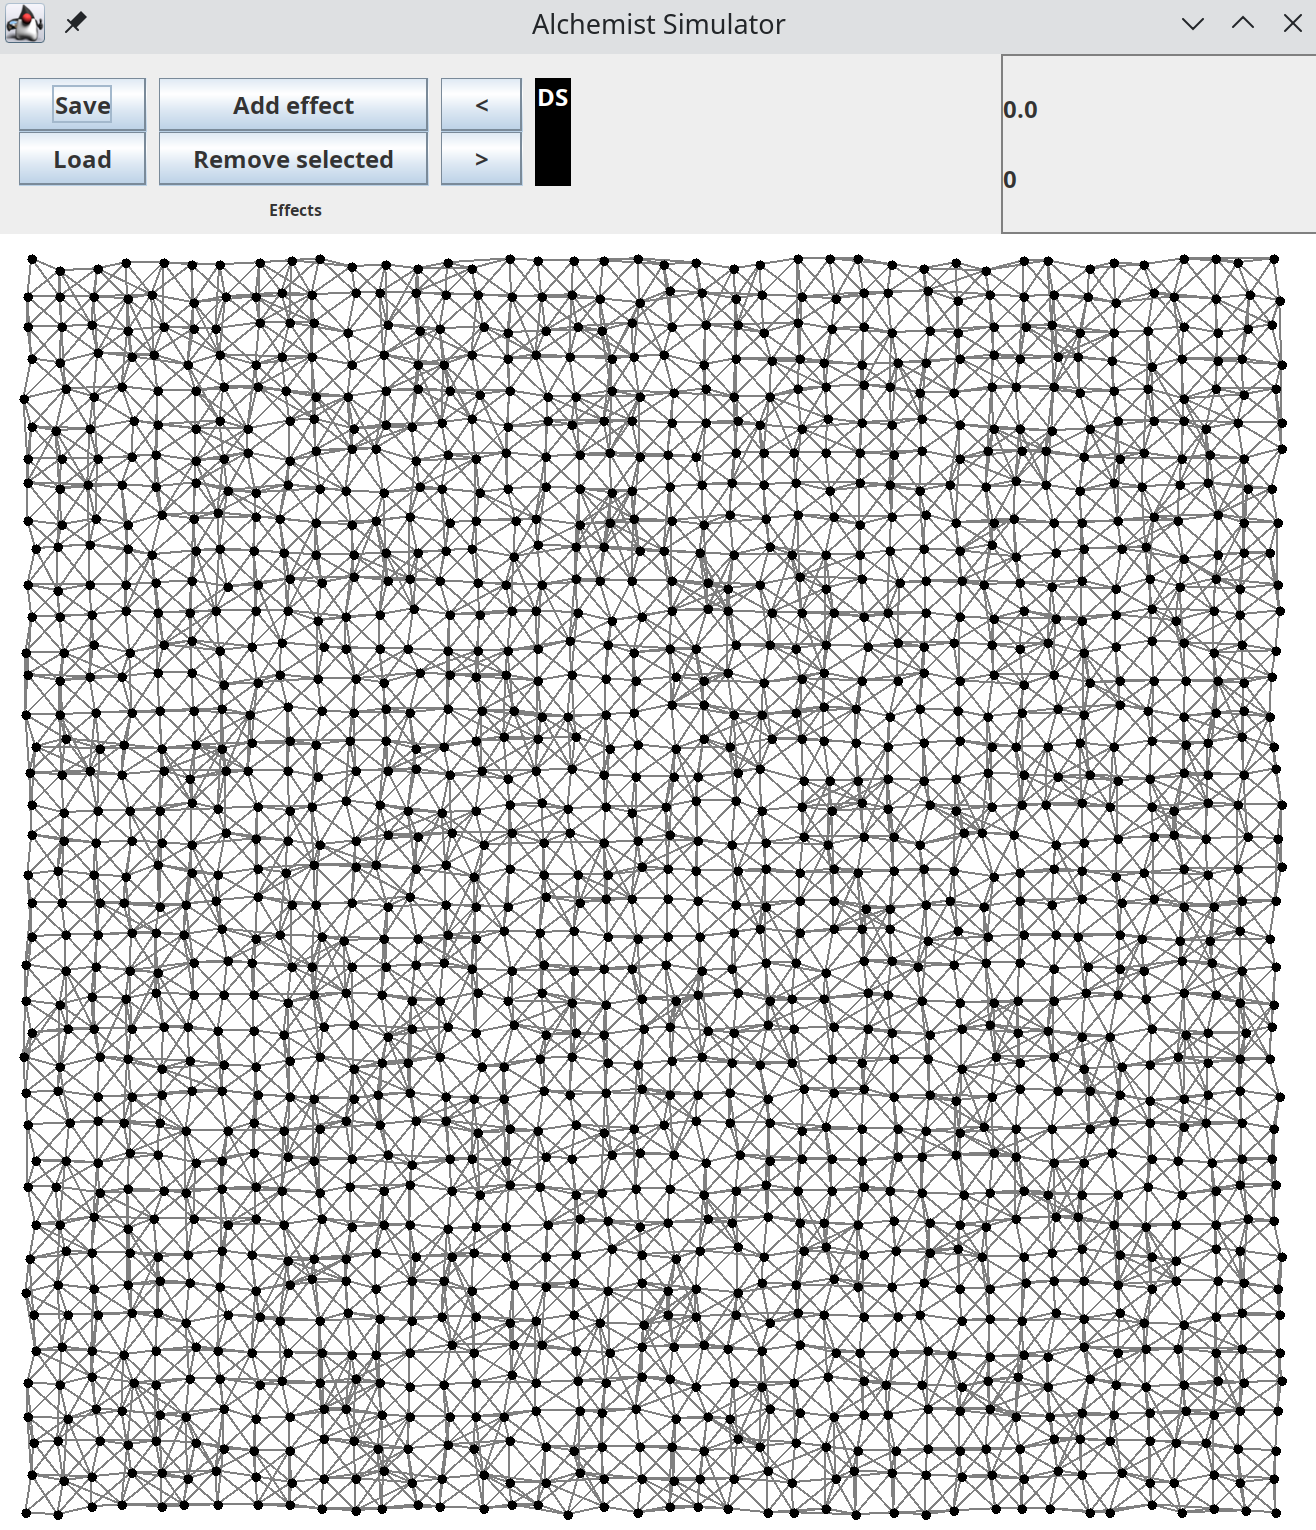
\includegraphics[width=\textwidth]{figures/alchemist.png}
    \end{subfigure}
    \caption{An Alchemist simulation example.}
    \label{fig:alchemist}
\end{figure*}

%----------------------------------------------------------------------------------------
\chapter{Requirements} 
\label{chap:requirements}
%----------------------------------------------------------------------------------------
This chapter first introduces the domain model of the \emph{hybrid AC-MARL} approach to engineer CPSWs, 
    and then presents the framework requirements. Finally, some scenarios
    are explained to provide a reference context.

\section{Domain model}
The proposed \emph{hybrid} approach between \emph{AC} and \emph{MARL} aims to combine the strengths of the two 
    approaches to engineer CPSWs.
    The idea is to leverage AC to define \emph{structural} rules of the swarm (e.g., leader election \cite{pianini2022self}) 
    while using MARL to define \emph{behavioral} rules (e.g., the choice of an action by an agent).
    Harnessing machine learning allows for the definition of more complex and adaptive behaviors, 
    which would be challenging to achieve through programmatic methods.

To accurately define the domain, a \emph{Domain-Driven Design} \cite{evans2004domain} approach was used. 
    First, the \emph{ubiquitous language}, as presented in \Cref{tab:ul}, was defined. 
    This associates a precise definition with each term of the domain, thereby 
    eliminating potential \emph{ambiguities}, which are common given the breadth of the MARL domain.

The \emph{environment} is the context in which \emph{agents} are immersed and operate, cooperating to solve the assigned task. 
    Agents interact with the environment by receiving the \emph{state} it is in before choosing which \emph{action} to perform,
    but they are also equipped with \emph{sensors} through which they can perceive certain features of the context they are in, 
    such as the number of other agents in the neighborhood and the distance from them.
    Each agent chooses which action to take based on its own behavior \emph{policy}. This policy is updated in accordance 
    with the \emph{system} that encompasses the agents themselves and the environment. This system is one of the key abstractions 
    and defines the execution flow of agents. For example, in a \emph{CTDE (Centralized Training and Decentralized Execution)}
    system, agents rely on a centralized learner that updates the policy as experience is accumulated and then also 
    distributes the new policy to each agent. On the other hand, in a \emph{DTDE (Decentralized Training and Decentralized 
    Execution)} system, each agent is responsible for its own policy, potentially resulting in each agent having a 
    different policy from all the others.

\begin{table}
    \centering
    \begin{tabularx}{\textwidth}{lX}
        \hline
        \textbf{\emph{Concept}} & \textbf{\emph{Definition}} \\
        \hline
        Environment & The context in which the \emph{agents} are immersed and operate,
                        it is a representation of the task to be solved.
                        It is capable of interacting with the agents, providing information
                        about its current \emph{state}, receiving the \emph{actions} that one or more agents
                        wish to execute, and returning the corresponding \emph{reward}. \\
        \hline
        Agent       & An entity that interacts within an \emph{environment} and with other \emph{agents}
                        in order to learn the optimal \emph{actions} sequence to maximize a \emph{reward} signal. 
                        It is equipped with \emph{sensors}, \emph{actuators} and a \emph{communication mechanism}. \\
        \hline
        State       & A representation of the \emph{environment} at a given time, 
                        including any relevant information that an \emph{agent} can perceive 
                        or use to make decisions about its \emph{actions}. \\
        \hline
        Action      & A decision or choice made by an \emph{agent} in response to the current 
                        state of the \emph{environment}. \\
        \hline
        System      & A collection of \emph{agents} that interact within a shared \emph{environment}. 
                        It defines the training and execution flow of the agents. \\
        \hline
        Policy      & A function that maps the current \emph{state} of the \emph{environment} to a probability 
                        distribution over the set of possible \emph{actions} that the \emph{agent} 
                        can take in that \emph{state}. The policy specifies the \emph{agent's} behavior 
                        or strategy in response to different \emph{states} of the \emph{environment}, 
                        and it is learned through a process of trial and error using the 
                        \emph{reward} signal as feedback. \\
        \hline
    \end{tabularx}
    \caption{Hybrid AC-MARL approach ubiquitous language}
    \label{tab:ul}
\end{table}

\section{Framework requirements}
This section describes the requirements that the project must satisfy. 
\begin{itemize}
    \item \emph{Business Requirements}: specify the characteristics that the system must possess in order to be correct;
    \item \emph{User Requirements}: express the needs of the users and describe the actions that the user should be able 
        to perform while interacting with the system;
    \item \emph{Functional Requirements}: concern the functionalities that the system must make available to the user. 
        Their definition should be based on the user requirements extracted previously;
    \item \emph{Non-Functional Requirements}: concern the functionalities that the system does not necessarily have 
        to possess in order to be functional and correct.

\end{itemize}

\subsection*{Business requirements}
The business requirements specify the characteristics that the system must have to be correct. Those identified for ScaRLib are:
\begin{itemize}
    \item The framework must enable the development of CMARL systems for JVM-based environments 
        through a high-level specification;
    \item The framework should support different training and execution models;
    \item The framework should be extensible and modular to allow  the integration of:
    \begin{itemize}
        \item different learning algorithms;
        \item different simulators;
        \item different deep learning frameworks.
    \end{itemize}
\end{itemize}

\subsection*{User requirements}
The user requirements express the needs of the users and describe the actions that the user must be able to perform by interacting with the system.
    From the previous domain analysis that was carried out, we can identify the following user requirements:
\begin{itemize}
    \item It should be possible to configure the learning system through a \emph{DSL};
    \item It should be possible to define a custom \emph{environment};
    \item It should be possible to define a custom \emph{state space};
    \item It should be possible to define a custom \emph{action space};
    \item It should be possible to define a custom \emph{reward function};
    \item It should be possible to define a custom \emph{neural network} to approximate the policy/value-function;
    \item It should be possible to define some of the agent logic through \emph{aggregate programming};
    \item It should be possible to log information related to the training process;
    \item It should be possible to visualize the execution of agents, both during training and testing.
\end{itemize}

\subsection*{Functional requirements}
The functional requirements relate to the functionalities that the system must make available to the user. 
    To define them, it is necessary to rely on the user requirements extracted previously.
\begin{itemize}
    \item The framework must allow the user to define their own \emph{experiment}, this includes: 
            i) the environment, 
            ii) the state space, 
            iii) the action space, and
            iv) the reward function;
    \item The framework must allow the user to define their own \emph{learning algorithm};
    \item The framework must allow the user to define their own \emph{neural network} to approximate the policy/value-function;
    \item The framework must allow the user to define their own \emph{agent logic} through aggregate programming;
    \item The framework must allow the user to log information related to the training process;
    \item The framework must allow the user to visualize the execution of agents, both during training and testing.
\end{itemize}

\subsection*{Non-functional requirements}
Non-functional requirements concern the functionalities that the system does not necessarily have to possess in order to ensure that it is correct.
The following non-functional requirements have been identified within the system to be developed:
\begin{itemize}
    \item The framework should provide an easy and clean API;
    \item The framework must be cross-platform, therefore it must be executable on any operating 
        system capable of supporting Java version 11 or later;
    \item The framework should be extensible and modular allowing the user to customize some of its 
        components (e.g., the simulator or the learning algorithm).
\end{itemize}

\section{Scenarios}

This section aims to provide a \emph{reference context} for the use of the framework by attempting to illustrate, 
    through some practical examples, the key characteristics within the domain of CPSWs.

The first scenario represents one of the simplest conceivable instances for CPSWs, in which the proposed hybrid 
    approach can be beneficial. It involves a \emph{fleet of drones}, each drone having a predetermined \emph{set of neighbors}. 
    The objective for each drone is to maintain proximity to its neighbors (i.e., \emph{cohesion}), while avoiding \emph{collisions}.

The second example also involves a fleet of drones but is more intricate than the previous one. In this case, 
    the fleet's purpose is to monitor a designated area of territory for \emph{adverse events} (e.g., fires). Once an adverse 
    event is identified, the fleet must \emph{coordinate} to determine the number of drones to intervene and their 
    respective \emph{strategies}.

A final example entails the use of \emph{wearable devices} (e.g., smartwatches) for \emph{crowd management} during a public event 
    (e.g., a conference or concert) in order to provide navigation directions to avoid congestion and to facilitate 
    evacuation in case of emergencies.


%----------------------------------------------------------------------------------------
\chapter{Implementation design} 
\label{chap:impl-design}
%----------------------------------------------------------------------------------------

This chapter presents the design decisions for modelling the domain and implementing 
    the framework. It introduces the key details of each module, followed by a discussion
    of the interactions between them.

\section{Framework architecture}

The framework has been devised to aid the development of CMARL systems in JVM-based environments through high-level 
    specifications. For this purpose, the tool is divided into three primary modules (\Cref{fig:mainmodules}), namely:
    i) \texttt{scarlib-core}:  which captures the core concepts of the CMARL domain by abstracting low-level 
        implementation details,
    ii) \texttt{dsl-core}: which provides a high-level language for specifying a CMARL system, and
    iii) \texttt{alchemist-scafi}: which provides bindings between ScaRLib and the Alchemist and ScaFi tools, enabling 
        experiments in a simulated environment using aggregate computing.
    One aspect to consider is the \texttt{pytorch} sub-module upon which \texttt{scarlib-core} relies. This sub-module serves as 
    a \emph{learning engine} to conduct training and optimization of neural networks utilised by the RL algorithms. 
    It's worth noting that, if required, an alternative substitute module (e.g., DL4J \footnote{\url{https://deeplearning4j.konduit.ai/}})
    that has similar functionality can be used instead.

The modularisation of the framework brings various benefits. On the one hand, the framework makes it possible 
    for the user to select only those components that are necessary for him. On the other hand, this makes it 
    easy to extend and modify the framework. For instance, ScaRLib, due to the actual need, has already 
    integrated the \texttt{alchemist-scafi} module. If a user wants to use another simulator instead of Alchemist 
    (e.g., FlameGPU \cite{flame} or VMAS \cite{bettini2022vmas}), he simply has to disable the import of this module and build a fresh 
    custom environment based on his chosen simulator.

\begin{figure}
    \centering
    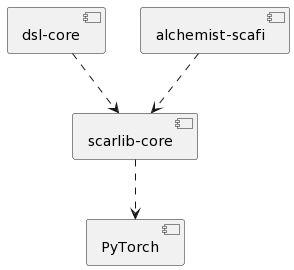
\includegraphics[width=0.4\textwidth]{figures/scarlib-modules.png}
    \caption{ScaRLib main modules.}
    \label{fig:mainmodules}
\end{figure}

\subsection*{ScaRLib Core}

The \texttt{scarlib-core} module contains the essential abstractions of the reference domain, including the necessary data structures 
    and learning algorithms. It has been conceptualised around several key components (\Cref{fig:uml-core}), the central one being the \emph{system}.
    \begin{figure*}[t]
        \centering
        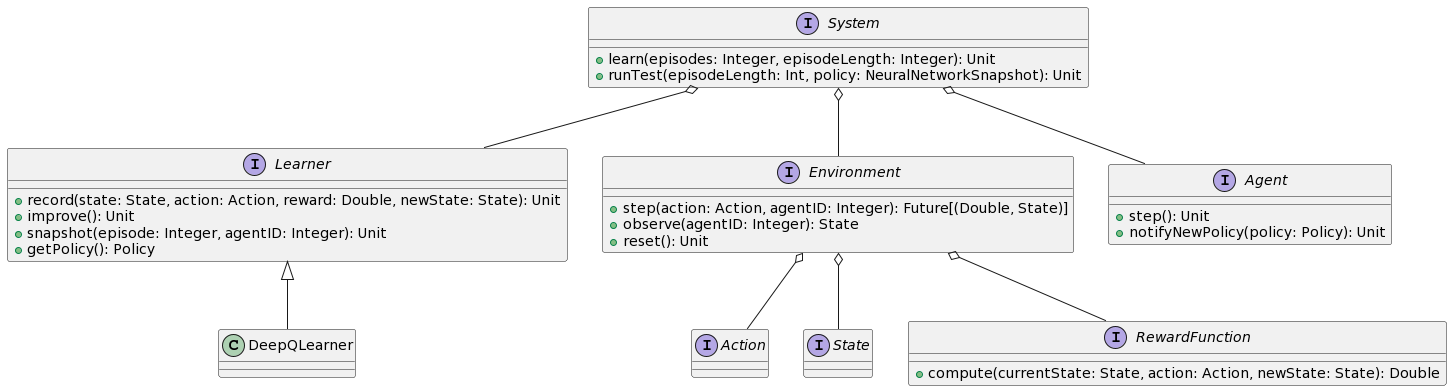
\includegraphics[width=\textwidth]{figures/uml-core.png}
        \caption{scarlib-core module UML class diagram.}
        \label{fig:uml-core}
    \end{figure*}
    A system serves as a generic representation of a collection of agents interacting with each other and with a shared 
    environment, trained to optimise a reward signal conveyed by a reward function. The tool offers two pre-implemented 
    systems that are widely used in literature \cite{Du2020}, namely the \texttt{CTDESystem} and \texttt{DTDESystem}. The distinction between them is based
    on the training of the different agents. To understand their dynamics better, it is useful to study their internal details. 
    Both systems undergo a training process that includes a specific number of \emph{epochs}, each of which comprises numerous \emph{episodes}. 
    Within a single episode, at a generic time step $t$, agents interact with the environment and receive the state $s_t$. 
    They choose which action $a_t$ to take based on this and the current policy $\pi_t$. The environment then gathers the 
    actions of all agents and returns a new state $s_{t+1}$ and the corresponding reward $r_{t+1}$. 
    When using a \texttt{CTDESystem}, the agents are trained in a centralised way, involving a specialised agent, called the \emph{Learner}, 
    that gathers the experience of all the other agents to update the policy, and then the updated policy is distributed to all 
    the agents,  resulting in a \emph{homogeneous} system. 
    Conversely, when using a \texttt{DTDESystem}, each agent assumes responsibility for individual policy training,
    thus making the policies different from each other, resulting in a \emph{heterogeneous} system. 
    The behaviors of these systems are depicted in \Cref{fig:systems}.
    
    \begin{figure*}[t]
        \centering
        \begin{subfigure}[b]{0.49\textwidth}
            \centering
            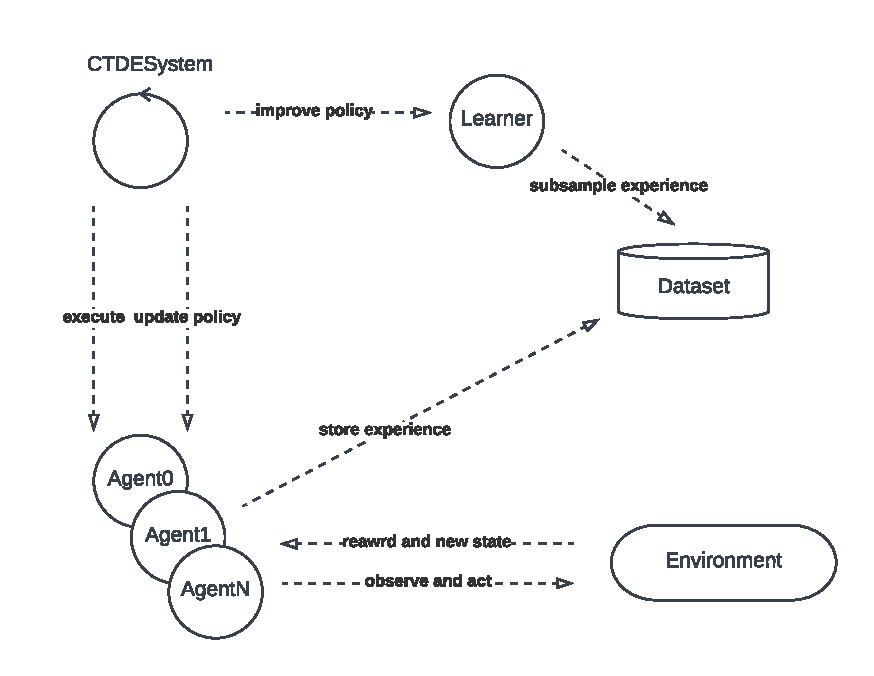
\includegraphics[width=\textwidth]{figures/ctdesystem.pdf}
            \caption{CTDE System}
        \end{subfigure}
        \begin{subfigure}[b]{0.49\textwidth}
            \centering
            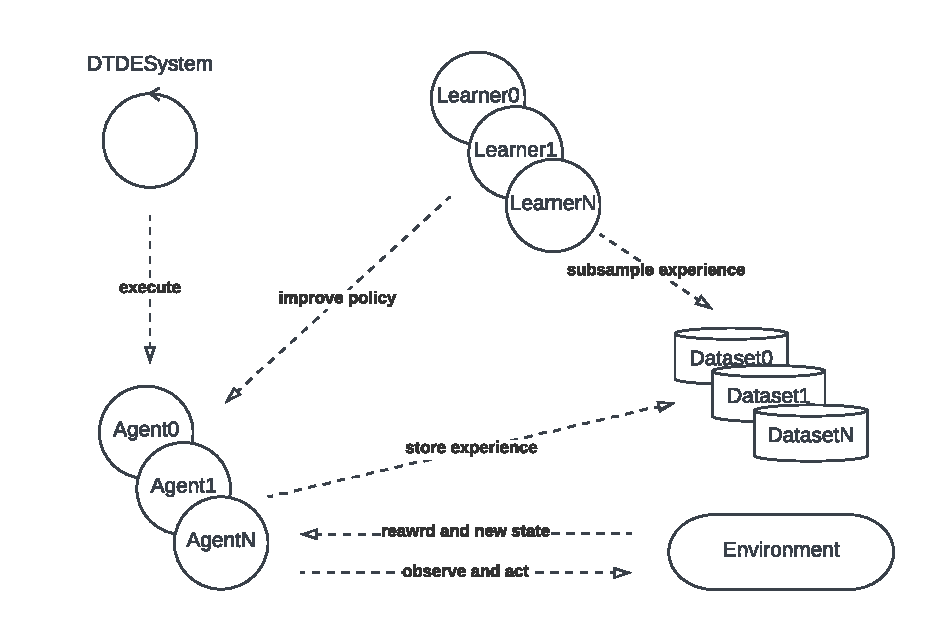
\includegraphics[width=\textwidth]{figures/DTDE.pdf}
            \caption{DTDE System}
        \end{subfigure}
    \caption{Examples of developed System dynamics. 
    On the left, there is the centralized system, 
    where a learner with a global view of the system 
    updates the policy shared with all agents. 
    %
    On the right, there is a decentralized system, 
    where each agent has a local policy and a local policy.}
    \label{fig:systems}
    \end{figure*}

Furthermore, the module provides a pre-implemented version of the DQN \cite{dqn} learning algorithm, which can be used 
    to train the agents. Alternatively, a user can define their own custom learning algorithm by creating a
    new class that extends the trait \texttt{Learner}.

\subsection*{DSL Core}
The \texttt{dsl-core} module is dedicated to implementing a \emph{Domain Specific Language} in Scala that can be used to 
    define the high-level configuration of the experiment to run. This module is the simplest of the three, 
    consisting of a series of \emph{contextual functions} that make the definition of the learning system 
    fluent and straightforward.
    The decision to implement a DSL, which essentially serves as a \emph{facade} for the abstractions defined 
    by the framework, was made to enable the identification of simple configuration errors at \emph{compile time} rather than waiting
    for execution to intercept them.

Let's take the example of a user who wants to define his own learning system for the experiment he wants to run 
    with the DSL. First of all, the basic components must be defined. To start with, a reward 
    function must be defined.
    \begin{lstlisting}
class MyRewardFunction extends CollectiveRewardFunction:
    override def computeReward(state: State, action: Action, nextState: State): Double = ...
    \end{lstlisting}
    Afterward, it will be necessary to define the action space, which can be done as follows, 
    leveraging Scala's \emph{product types}:
    \begin{lstlisting}
sealed trait CustomAction extends Action
object CustomActionSpace:
    case object A extends CustomAction
    case object B extends CustomAction
    case object C extends CustomAction
    def all: Seq[CustomAction] = Seq(A, B, C)
    \end{lstlisting}
Final refinements required include: 
    i) choosing the class of the Alchemist environment to instantiate, 
    ii) defining the number of agents living in the chosen environment, and 
    iii) defining the size of the buffer in which the memory will be stored.
    Finally, everything can be combined to create the configuration of the learning system through the DSL 
    as follows:
\begin{lstlisting}
val system = learningSystem {
    rewardFunction { new MyRewardFunction() }
    actions { CustomActionSpace.all}
    dataset { ReplayBuffer[State, Action](10000) }
    agents { 50 } // select the number of agent
    environment {
        // select a specific environment
        "it.unibo.scarlib.experiments.myEnvironment"
    }
}
\end{lstlisting}

\subsection*{Alchemist-ScaFi}

The \texttt{alchemist-scafi} (\Cref{fig:alchemist-scafi}) module has been designed to provide integration between the \texttt{scarlib-core} module 
    and the two tools \emph{Alchemist} \cite{alchemist} and \emph{ScaFi} \cite{casadei2022scafi}. 
    In addition to the \texttt{scarlib-core} module, this module provides an environment that implements bindings 
    with the Alchemist simulator. This way, the user only needs to provide a YAML file containing the 
    simulation specification they want to execute. 
    Another component is the abstract class \texttt{ScafiProgram}, which represents the logic of the agents. 
    In this case, the user only needs to implement the \texttt{computeState} method, specifying through \emph{aggregate 
    computing} how to reconstruct the state that will be returned to the various agents.

\begin{figure*}[t]
    \centering
    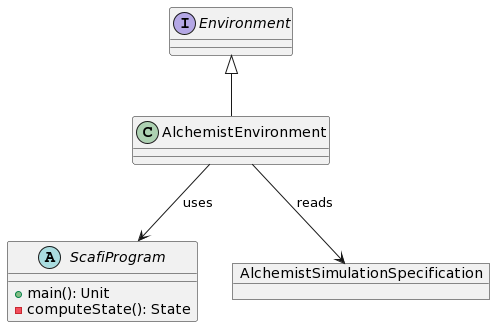
\includegraphics[width=0.7\textwidth]{figures/alchemist-scafi-uml.png}
    \caption{alchemist-scafi module UML class diagram.}
    \label{fig:alchemist-scafi}
\end{figure*}

\section{Component interactions}

The \emph{interaction} among the various components depends on the selected \emph{training and execution model}. 
    The framework provides two pre-implemented models, namely: \texttt{CTDESystem} and \texttt{DTDESystem}. 
    The interaction flow for the CTDE model is illustrated in \Cref{fig:ctde-sequence}, while that for the DTDE model is shown in
    \Cref{fig:dtde-sequence}. In general, the main interaction takes place between the \emph{agents} and the \emph{environment}, in both models: 
    initially, the agent observes the state of the environment and, based on this observation, 
    makes a query to its policy to choose an action to execute. When the action is received, the environment computes 
    the new state and returns a reward and the new state to the agent.
    At this point, the most significant difference between the two systems becomes evident. In the case of CTDE, the agent collects its experience 
    in a centralized Learner that takes responsibility for updating the policy following the implemented learning algorithm. Conversely, in the case of 
    DTDE, each agent interfaces directly with its own learner. In the former case, the policies of various agents will be homogeneous, 
    whilst in the latter case, each agent will have its own policy.

An important aspect to note regarding figures \ref{fig:ctde-sequence} and \ref{fig:dtde-sequence} is that they represent a simplification of what actually happens. 
    In fact, only one agent is illustrated, while in reality, the number of agents is much greater than $1$. Both systems manage agents \emph{concurrently}, 
    leveraging asynchronous programming to enable parallel execution. The environment, in order to compute the new state,
     must wait to collect the actions of all agents for the current time step.

\begin{figure*}[t]
    \centering
    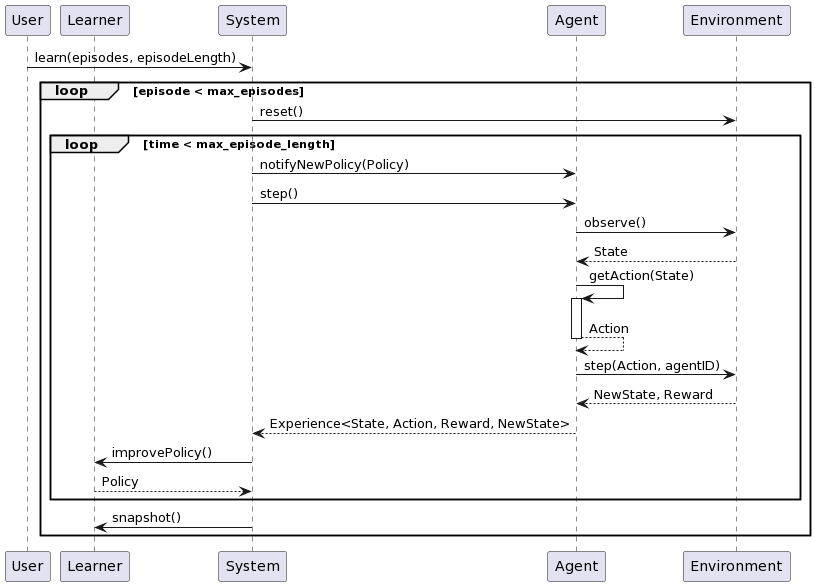
\includegraphics[width=0.8\textwidth]{figures/CTDE-System-Sequence-Diagram.png}
    \caption{UML sequence diagram of the learning process using a CTDE system.}
    \label{fig:ctde-sequence}
\end{figure*}

\begin{figure*}[t]
    \centering
    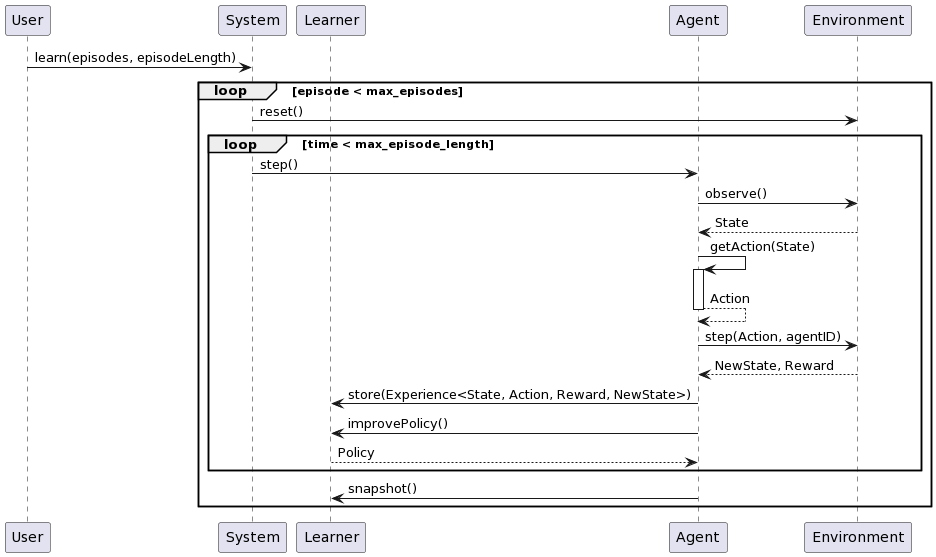
\includegraphics[width=0.8\textwidth]{figures/DTDE-System-Sequence-Diagram.png}
    \caption{UML sequence diagram of the learning process using a DTDE system.}
    \label{fig:dtde-sequence}
\end{figure*}

%----------------------------------------------------------------------------------------
\chapter{Project} 
\label{chap:project}
%----------------------------------------------------------------------------------------
\section{Technologies used in the project}

\subsection*{Scala language}

\emph{Scala} (short for \emph{Scalable Language}) is a general-purpose programming language. 
    It combines the \emph{object-oriented} paradigm with the \emph{functional} paradigm. The language is purely object-oriented 
    in that \emph{every value is an object}, while also incorporating the functional paradigm, ensuring 
    that \emph{every function is a value}. This permits the utilisation of higher-order functions, anonymous functions, and 
    lambdas in a straightforward and natural manner, fostering programmers to implement pure functions. This implies that, 
    for identical inputs, they returns the same output without side effects. This facilitates the implementation of more easily 
    comprehensible and maintainable code with fewer errors.

The Scala language has been designed for the succinct, elegant, and type-safe expression of commons programming patterns. 
    It is a \emph{statically-typed} language, and due to the expressiveness of its type system, its abstractions can be 
    used reliably and safely. Some of these abstractions include: upper and lower bounds for types, variance annotations, 
    implicit parameters, implicit conversions, as well as polymorphic methods, among others.
    Moreover, a very important feature of the compiler is its highly potent \emph{type inference}, 
    which makes the code very readable, allowing programmers to avoid using unnecessary and redundant type annotations.

Originally, Scala was designed as a language intended for seamless interoperability with the JVM (Java Virtual Machine). 
    Since then, native versions and interoperability with JavaScript have also been included. The compiler does not directly 
    manage support for cross-platform development; it is achieved by using plugins. These plugins enable the creation of an 
    intermediate representation that contains cross-platform aspects, which is then used to generate the final code.

\subsection*{Asynchronous programming}
\emph{Asynchronous programming} is crucial within modern software development. The importance of asynchronous programming is its 
    potential to improve the efficiency and responsiveness of applications. By permitting tasks to run concurrently without 
    blocking the primary execution thread, it allows applications to handle multiple operations at once, making them more 
    scalable and responsive to user interactions.
    In Scala, \emph{Future} and \emph{Promise} are crucial devices for handling asynchronous operations. 
    A future denotes a value or error computation that may finish at some point in the future, allowing non-blocking execution.
    A promise, conversely, performs as a writable, synchronized container for a future result. 
    This pairing encourages orderly and articulate code for dealing with asynchronous tasks, 
    encouraging a more natural and manageable codebase.

\subsection*{ScalaPy}
\emph{ScalaPy} \footnote{\url{https://scalapy.dev/}} is a software tool that effectively integrates Python and Scala, 
    two prominent programming languages. This bridge empowers developers to utilise the strengths of both languages 
    in a single project, offering flexibility and extensibility required for various tasks.
    At its heart, ScalaPy permits developers to utilise Python libraries and packages directly in Scala code, 
    removing the requirement for challenging interoperability workarounds. This capability is notably beneficial 
    when harnessing the extensive Python ecosystem, which comprises libraries for data science, machine learning, 
    and scientific computing, such as NumPy, Pandas, and TensorFlow. By bridging this gap, ScalaPy enables Scala developers
    to tap into the rich functionality and pre-existing solutions offered by the Python community, thereby accelerating 
    development and reducing duplication of effort.
    Moreover, ScalaPy provides robust support for data type conversions, allowing seamless passage of data between 
    Python and Scala, further enhancing the interoperability between the two languages. This capability simplifies 
    the process of combining Python's dynamic typing with Scala's strong, static typing, ensuring that the integration 
    remains type-safe and reliable.

\subsection*{PyTorch}

\emph{PyTorch} \cite{imambi2021pytorch} has become a groundbreaking framework for training \emph{deep neural networks}, providing a 
    potent and adaptable platform which has won over both researchers and developers in the field of deep learning. 
    PyTorch's dynamic computation graph, sophisticated design, and user-friendly interface distinguish it from the rest, 
    making it an indispensable tool for building and training neural networks.
    At the heart of PyTorch's appeal is its \emph{dynamic computation graph}, a sharp contrast to the static graphs seen in many 
    other deep learning frameworks. This dynamic nature allows developers to define and revise computational graphs as
    needed, empowering dynamic control flow and simplifying debugging. Researchers find this feature particularly useful 
    in implementing complex models, encouraging experimentation and streamlining prototyping.
    PyTorch's capacity to harness \emph{GPU acceleration} is effortless, allowing for the training of deep neural networks on 
    \emph{high-performance hardware}. \emph{Autograd}, an automatic differentiation engine, effectively calculates 
    gradients for optimization algorithms based on gradients such as \emph{stochastic gradient descent} \cite{amari1993backpropagation}. 
    This characteristic streamlines the implementation of custom loss functions and intricate optimization strategies.

\section{DevOps techniques}

\emph{DevOps} techniques are fundamental to the development of a project for several reasons. On the one hand, 
    they make it possible to improve code quality while keeping work organised, promoting testing and 
    ensuring continuous integration of the various components being developed, while systematically 
    tracking released versions. On the other hand, they make it easier to maintain high productivity 
    by avoiding downtime and automating repetitive and tedious tasks that can be performed more efficiently 
    by a computer than by a human, leaving more time for critical features.

\subsection*{Repository management}
The management of the codebase was carried out using the renowned \emph{Decentralized Version Control System (DVCS)} git \cite{spinellis2012git}, 
    specifically leveraging the \emph{GitHub} \footnote{\url{https://github.com/}} hosting service. To ensure standardized and consistent tool usage, 
    avoiding errors and compatibility issues, the \emph{GitFlow} methodology was chosen.
    GitFlow is a branching model that involves the use of two main branches: \texttt{master} and \texttt{develop} (\Cref{fig:gitflow}).
    \begin{figure*}[t]
        \centering
        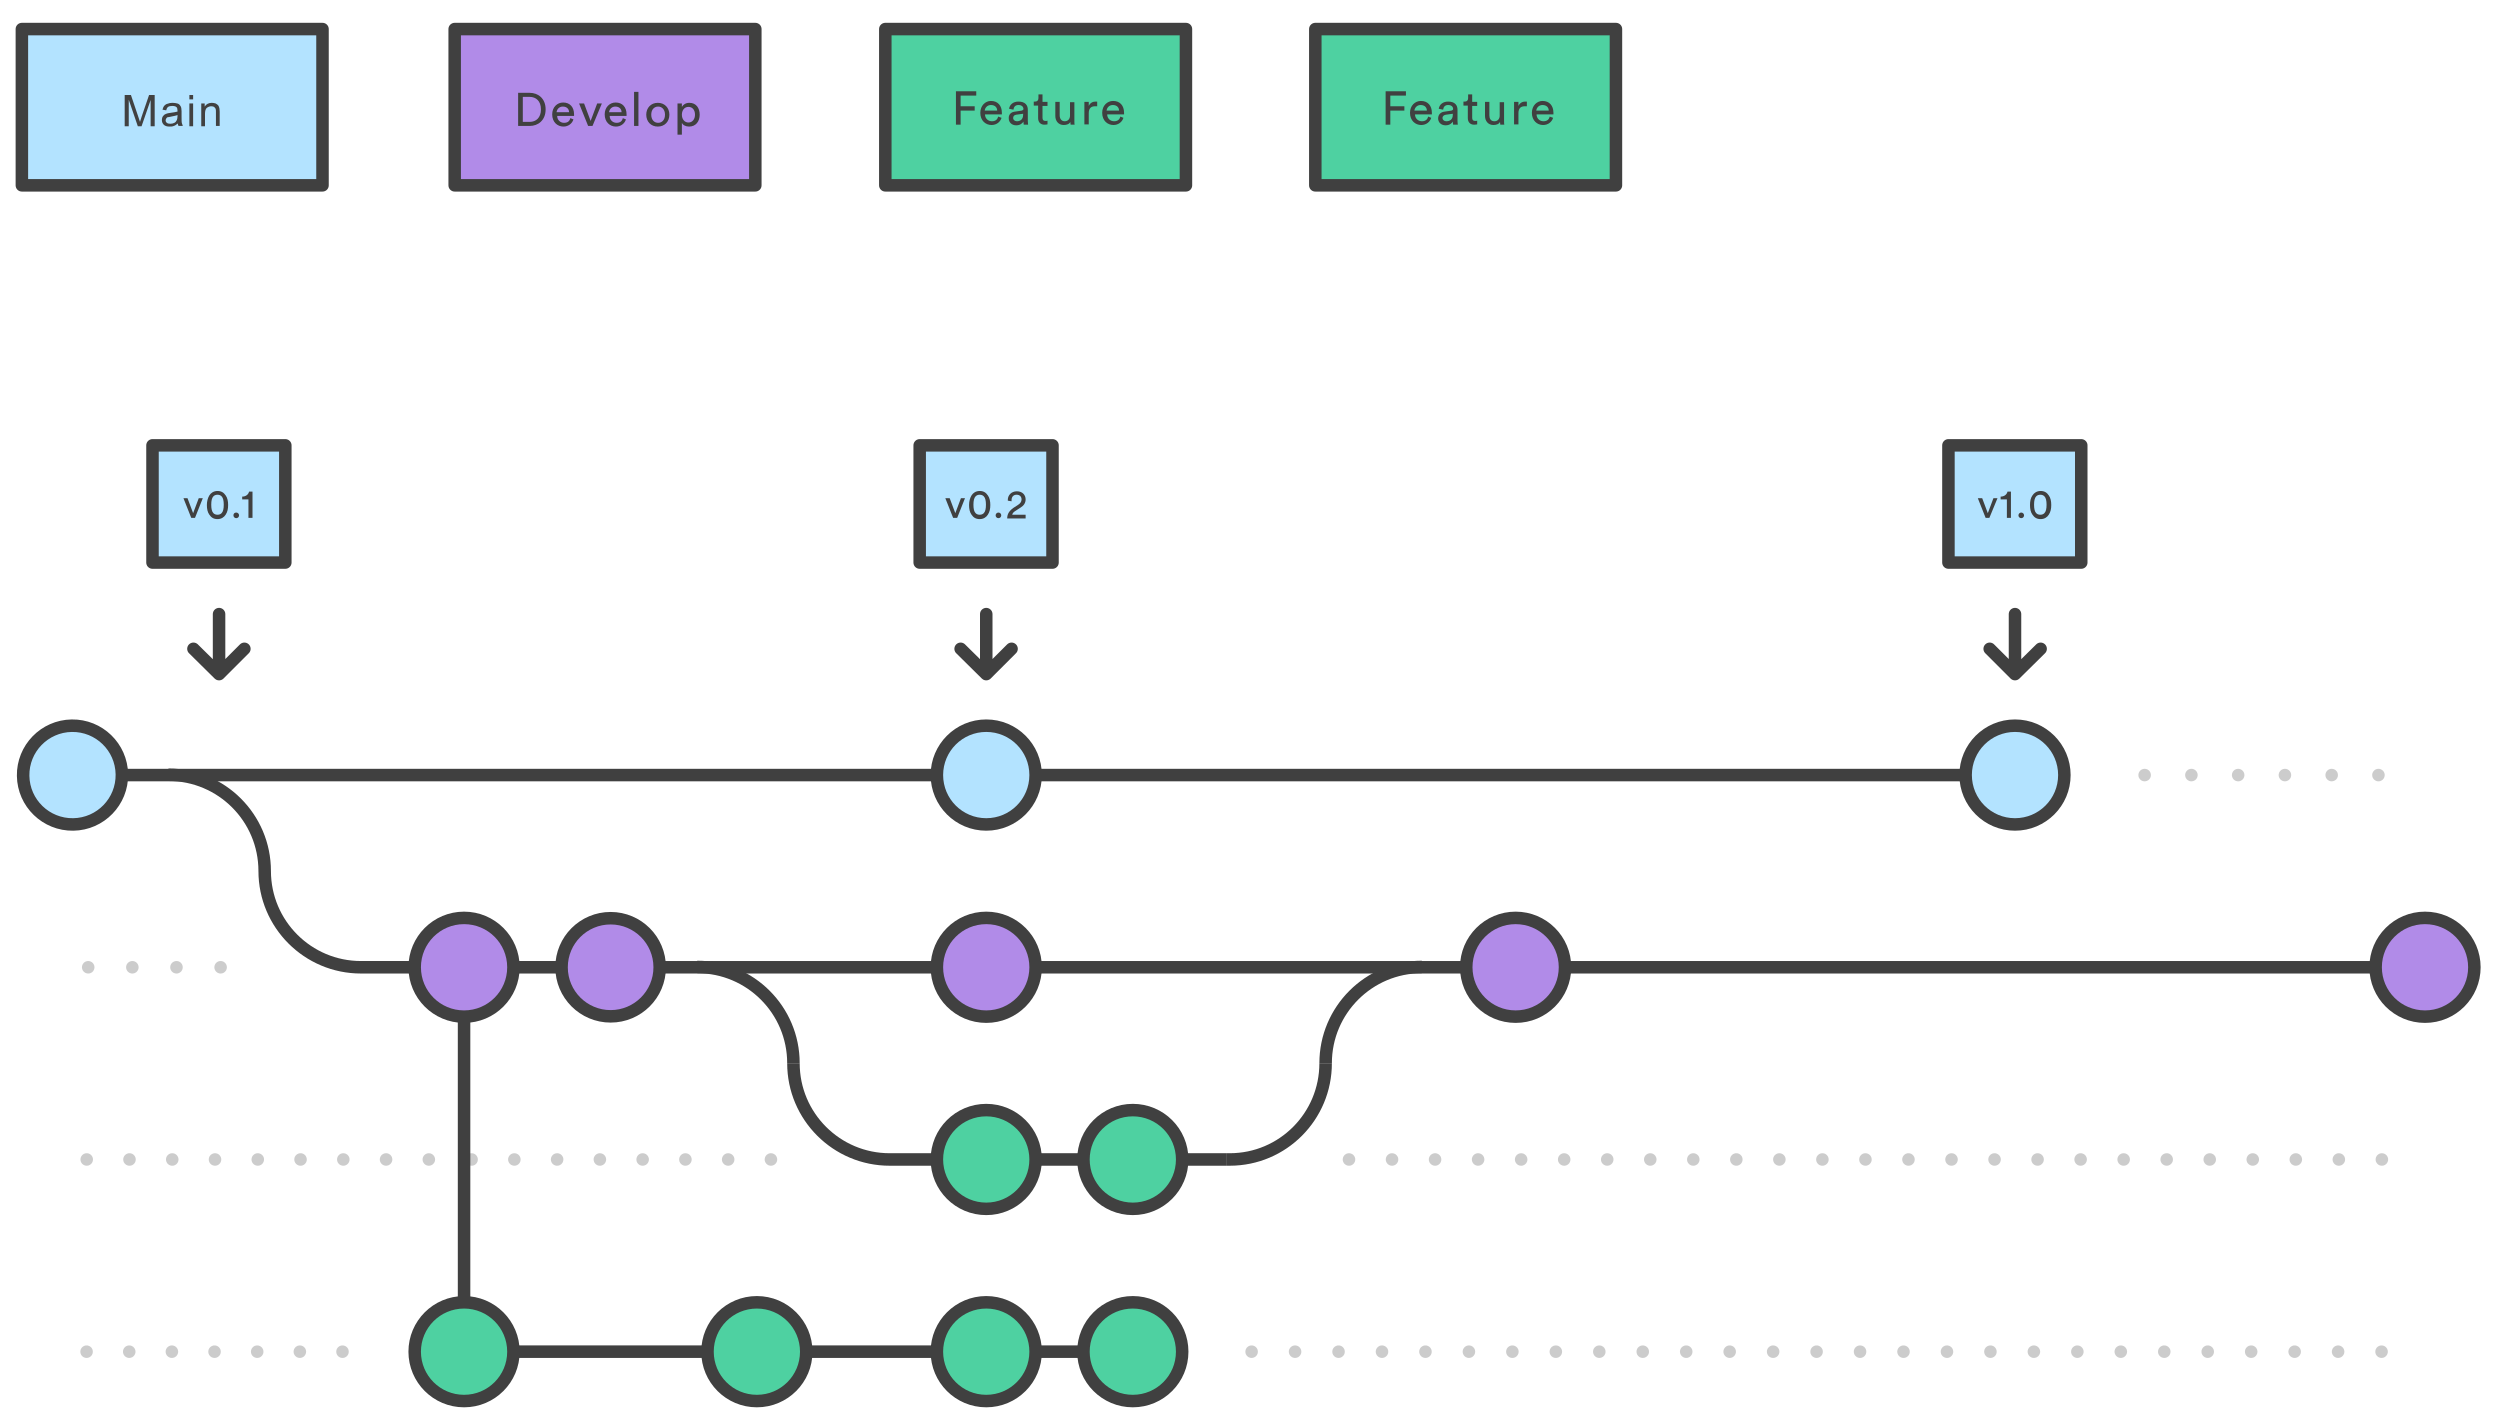
\includegraphics[width=0.8\textwidth]{figures/gitflow.png}
        \caption{GitFlow.}
        \label{fig:gitflow}
    \end{figure*}
    The \texttt{master} branch is used for \emph{releases}, while the \texttt{develop} branch is used for \emph{ongoing development}. 
    Additionally, for each feature, a branch named \texttt{feature/feature-name} is created, which is then merged 
    into the \texttt{develop} branch once the feature is completed.
    Furthermore, to ensure a standardized way of writing commit messages, 
        the \emph{Conventional Commits} \footnote{\url{https://www.conventionalcommits.org/en/v1.0.0/}} 
        approach was adopted. A commit is therefore written in the following format: \texttt{<type>[<optional scope>]: <description>}.
        Some examples of commit types are \texttt{feat}, \texttt{fix}, \texttt{docs} and \texttt{style}.
\subsection*{Build automation}

\emph{Build automation} aims to automate the \emph{management of dependencies}, \emph{compilation}, and 
    \emph{distribution} of a software project.
    Firstly, build automation decreases human errors during source code compilation by eliminating potential 
    sources of errors from manual omissions or configuration mistakes. This increases the software's reliability 
    and accelerates the development cycle, enabling developers to concentrate on more creative tasks and 
    problem-solving instead of manual compilation.
    Additionally, build automation aids in the regulation of \emph{project dependencies} and \emph{version control}, 
    permitting developers to explicitly and systematically establish the necessary libraries and resources 
    for the application and guaranteeing that they persistently maintain the accurate versions.
    Finally, build automation facilitates \emph{continuous integration and continuous delivery (CI/CD)},
    which are essential for timely releases of new features and bug fixes. 
    Through automation, it is possible to implement \emph{automated testing} and continuous deployment processes, 
    decreasing release times and enhancing the overall quality of the software.

In this project \emph{Gradle} \footnote{\url{https://gradle.org/}} was used as the build automation tool. 
    It is a powerful and versatile tool extensively used in the software development industry. 
    It supplies a flexible and efficient approach to regulate and automate different aspects of the build 
    process for projects of all sizes and complexities. One of Gradle's notable advantages is its backing 
    for multiple programming languages and platforms, which renders it a preferred choice for both 
    Java-based applications and a wide variety of other technologies. With Gradle, 
    developers are able to establish and adapt build scripts by utilising a Kotlin-based DSL 
    (Domain Specific Language), providing considerable versatility and expressiveness. 
    Gradle also performs exceedingly well in dependency management, allowing developers to simply 
    declare and manage project dependencies, making it an essential tool for building and maintaining 
    strong software projects. Whether building, testing or deploying applications, Gradle streamlines 
    and automates these tasks to enhance productivity and allow developers to concentrate on 
    writing superior code.
    Most of the Gradle configuration is in the \texttt{build.gradle.kts} file.
    For example, it's possible to specify a dependency on an third-party library as shown below:
\begin{lstlisting}[language=kotlin]
dependencies {
    implementation("it.unibo.alchemist:alchemist-incarnation-scafi:25.14.6")
}
\end{lstlisting}
    Another crucial aspect is the ability to define custom tasks, allowing for a series of actions
    to be carried out during the build stage. For instance, the following task creates a jar
    file that holds the documentation of the program's code.
\begin{lstlisting}[language=kotlin]
val scaladocJar by tasks.registering(Jar::class) {
    dependsOn("scaladoc")
    val destinationDirectory = tasks
            .named<ScalaDoc>("scaladoc")
            .get()
            .destinationDir
    from(destinationDirectory)
    archiveClassifier.set("docs-${project.name}")
}
\end{lstlisting}

\subsection*{Continuous integration}
\emph{Continuous Integration (CI)} is a software development technique that involves regularly integrating code modifications into a 
    shared repository following automated building and testing procedures. 
    Its significance lies in its ability to optimise the development workflow by pinpointing and resolving problems early on 
    in the development cycle. CI ensures that modifications made by multiple developers do not cause any conflicts or bugs. 
    This improves code quality, reduces integration issues, and ultimately speeds up the software delivery. 
    By automating these processes, CI not only saves time but also encourages collaboration and motivates developers 
    to write reliable and maintainable code. This results in a more efficient and robust software development pipeline.

In this project \emph{GitHub Actions} \footnote{\url{https://docs.github.com/en/actions}} were used to implement CI. 
    GitHub Actions is a \emph{CI/CD service}, integrated into GitHub, that allows developers to automate their software development workflows. 
    GitHub Actions is based on the concept of \emph{workflows}, which are a series of jobs that are executed when a specific event occurs. 
    For example, a workflow can be triggered when a pull request is opened or when a commit is pushed to the repository. 
    Workflows are defined in a YAML file called \texttt{.github/workflows/main.yml}. 
    The following is an example of a workflow that is triggered when a commit is pushed to the \texttt{main} branch. It is composed 
    of one job named \texttt{build} that runs on a \texttt{ubuntu} machine. The job consists of four steps: first it checks out the code, 
    then it sets up the Node.js environment, then it installs project dependencies, and finally it runs the tests.

\begin{lstlisting}[language=yaml]
name: Simple Pipeline

on:
  push:
    branches:
      - main

jobs:
  build:
    runs-on: ubuntu-latest

    steps:
    - name: Checkout Code
      uses: actions/checkout@v2

    - name: Set up Node.js
      uses: actions/setup-node@v2
      with:
        node-version: '14'

    - name: Install Dependencies
      run: npm install

    - name: Run Tests
      run: npm test
\end{lstlisting}

\subsection*{Versioning and releasing}

\emph{Software versioning} refers to the process of assigning a unique identifier to a software state. 
    The identifier is typically an alphanumeric sequence of characters separated by dots, slashes, or dashes.
    In this project, to distinguish different versions of the software, we decided to follow the guidelines 
    proposed by \emph{Semantic Versioning} \footnote{\url{https://semver.org/}}. 
    Consequently, the software version is represented by three numbers separated by a dot: \texttt{MAJOR.MINOR.PATCH}.

The correct version to be associated with the software state is based on the saved commits, 
    which were written following the Conventional Commit approach. In particular, we used the following approach:
    \begin{itemize}
        \item \textbf{MAJOR} release: any commit type and scope that causes a breaking change;
        \item \textbf{MINOR} release: any commit with type \texttt{feat};
        \item \textbf{PATCH} release: any commit with type \texttt{fix}, \texttt{doc}, \texttt{perf}, \texttt{revert}.
    \end{itemize}

With regard to the \emph{release} of the software, on the other hand, it was decided to publish the various versions 
    on the \emph{Maven Central repository} \footnote{\url{https://central.sonatype.com/}}, so as to make the framework easily available and importable for all users.  
    The release process, following good devops practices, was also fully automated.


\section{License}

A \emph{software license} is a legal agreement that governs the terms and conditions under which a user may use a particular piece of software.
    It serves as a critical tool in the world of software development and distribution because it defines the rights and responsibilities of both 
    the software creator (licensor) and the end user (licensee). The importance of a software licence lies in several key aspects. 
    First, it helps protect the software developer's intellectual property rights by specifying how the software can be used, copied,
    modified and distributed. This ensures that the developer retains control over his or her creation and can potentially generate 
    revenue from it. Secondly, a well-drafted licence can provide legal protection for both parties by clarifying liability and warranty 
    terms, thereby reducing the risk of disputes and litigation. Finally, software licences can promote responsible and ethical use of 
    software by preventing piracy and unauthorised distribution, which ultimately benefits the software industry as a whole and 
    encourages innovation. In summary, software licences are essential because they provide a framework for fair, legal and mutually 
    beneficial interactions in the software ecosystem.

\paragraph{ScaRLib license} 
ScaRLib is distributed under the \emph{MIT license}. 
The \emph{Massachusetts Institute of Technology License}, commonly referred to as the MIT License, is an open-source software license 
    that has gained widespread use. Its simplicity and permissiveness enable developers to utilise, adjust, distribute, and even 
    commercialise the software without significant restrictions. Users are usually expected to include the original copyright notice 
    and disclaimer when redistributing the software. This licence advocates \emph{collaboration} and \emph{code sharing} 
    within the \emph{open-source community} while ensuring legal protection for creators and users. Its straightforward terms make it a 
    popular choice for developers intending to utilise or contribute to open-source projects.

%----------------------------------------------------------------------------------------
\chapter{Validation} 
\label{chap:validation}
%----------------------------------------------------------------------------------------
To test the functionalities of the framework, a series of experiments were created using selected 
    features from well-known problems in literature. This allowed for a large number of 
    agents to be involved and non-trivial coordination tasks to be undertaken.

\section{Cohesion and collision}

\paragraph{Description}
The aim of this experiment is to create a flock of drones with the task of avoiding \emph{collisions}
    and maintaining a \emph{cohesive} movement pattern. The goal is to learn a policy that guides each
    agent's movement based on the distances from neighbors.
    This problem is well-known in the literature as \emph{flocking} \cite{DBLP:conf/siggraph/Reynolds87,inverserl}.

In our study, we examine an unbounded 2D environment where every agent has a set number of neighbours 
    (the five nearest, a hyper-parameter that is configurable), and can move in eight directions 
    (the four cardinal points and the four diagonals). The state of the environment is reconstructed 
    through aggregate computing, using ScaFi, as follows:
\begin{lstlisting}
    val state = foldhoodPlus(Seq.empty)(_ ++ _)(Set(nbrVector))
\end{lstlisting}    
In the code above: 
    i) \texttt{nbrVector} represents relative distances to neighbours, 
    ii) \texttt{foldhoodPlus} is a ScaFi function that iterates over all neighbours, and
    iii) \texttt{++} is the concatenation operation between sequences.
 
A crucial aspect of this task involves defining the \emph{reward function}. 
    The aim is to learn a policy that enables agents, initially placed randomly within the environment, 
    to approach one another and reach a specific \emph{target distance} $\delta$ (set in advance as a parameter of the 
    experiment) without any collisions occurring. In this case, a function composed of two components 
    was selected. The \emph{collision factor} kicks in when the distance is less than the target distance:

    \begin{equation}
        \label{eq:collision-factor}
        \begin{split}
            \text{collision} = \begin{cases}
                0 & \text{if } d > \delta \\
                \exp\left(-\frac{d}{\delta}\right) & \text{otherwise}
            \end{cases}
        \end{split}
    \end{equation}
    Following this function, the distance $d$ from the nearest neighbour is \emph{exponentially weighted}, 
    causing agents to move away from each other.
    The second element aims to enhance \emph{cohesion}. Considering the neighbour with the longest distance $D$, 
    the reward function is defined as follows:
    \begin{equation}
        \text{cohesion} = \begin{cases}
            0 & \text{if } d < \delta \\
            -(D - \delta) & \text{otherwise}
        \end{cases}
    \end{equation}
    The overall reward function is defined as the sum of these two factors $(cohesion + collision)$ as shown in \Cref{fig:cc-rf}.

    \begin{figure}[t]
        \centering
        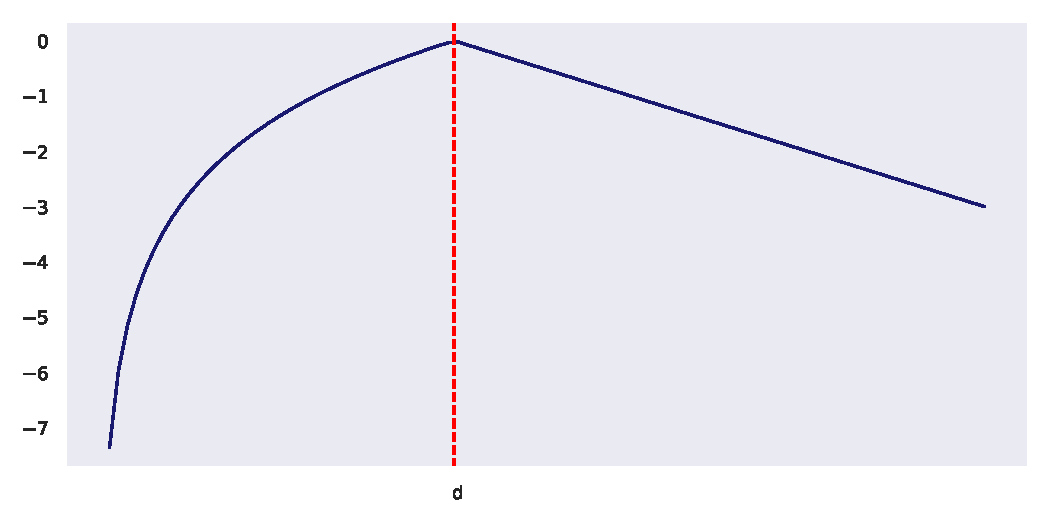
\includegraphics[width=0.6\textwidth]{figures/ccreward.pdf}
        \caption{Cohesion-Collision reward function: the red vertical line represents the target distance $d$.
            The portion of the graph to the right of the red line represents the influence of the cohesion term,
            while the left one represents the influence of the collision term.
        }
        \label{fig:cc-rf}
    \end{figure}

\paragraph{Results}
The experiment's training involved conducting 1000 \emph{epochs}, each with 100 \emph{episodes}, using 50 \emph{agents}, an 
    \emph{environment} measuring 50x50 metres and a \emph{target distance} $\delta$ set to 2 metres. The training was conducted 
    using both \emph{CTDE} and \emph{DTDE} processes.

\Cref{fig:cc-results} shows the \emph{multi-objective} nature of the problem. In fact, cohesion and collision are two \emph{adverse signals},
    and the system had to find a \emph{balance} between these two values. The graphs show that the learning algorithm optimizes one signal 
    at a time, with cohesion tending towards zero and collision increasing. Nonetheless, after $500$ epochs in CTDE simulation, 
    it is possible to see that the system had already found a balance between these two factors. 
    Instead, in the case of DTDE learning, convergence can be observed after approximately $50$ epochs, 
    which is due to the presence of a larger number of policies.

To verify the \emph{homogenous policy} learned using the CTDE process, $16$ simulations were conducted, each with agents randomly 
    positioned and varying the seeds. Given the homogenous nature of the policy learned with CTDE, we also varied the \emph{number 
    of agents} by conducting simulations with $50$, $100$ and $200$ agents. According to our \emph{hypotheses}, 
    this should not impact the \emph{quality} of the learned policy and its \emph{performance}.
    \Cref{fig:simulation-snapshots} displays screenshots from a simulation with $50$ and $200$ agents, illustrating how they gradually form \emph{cohesive clusters} 
    over time. \Cref{fig:test} shows the performance of the learned policy with $50$, $100$ and $200$ agents. From these graphs, it can 
    be observed that the \emph{performance does not change significantly} with varying numbers of agents, and the system is able to 
    maintain approximately a distance $\delta$ between the agents.

    \begin{figure*}[t]
        \centering
        \begin{subfigure}[b]{0.32\textwidth}
            \centering
            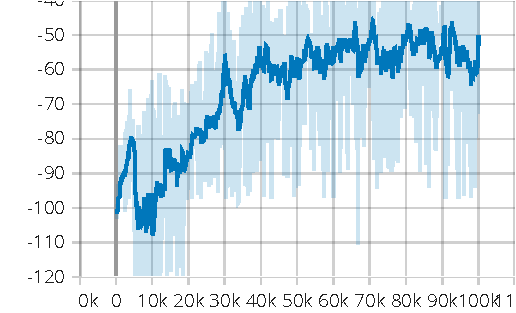
\includegraphics[width=\textwidth]{figures/reward-ctde.pdf}
            %\caption{Total average reward}
            %\label{fig:reward-cc}
        \end{subfigure}
        \hfill
        \begin{subfigure}[b]{0.32\textwidth}
            \centering
            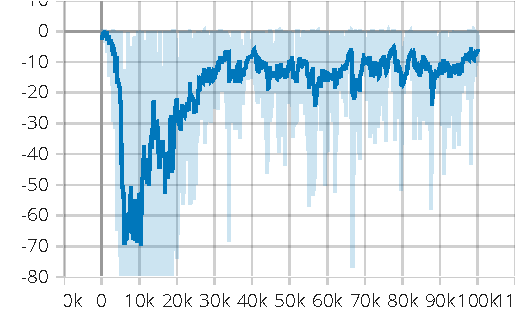
\includegraphics[width=\textwidth]{figures/collision-ctde.pdf}
            %\caption{Average collision factor}
            %\label{fig:collision-cc}
        \end{subfigure}
        \hfill
        \begin{subfigure}[b]{0.32\textwidth}
            \centering
            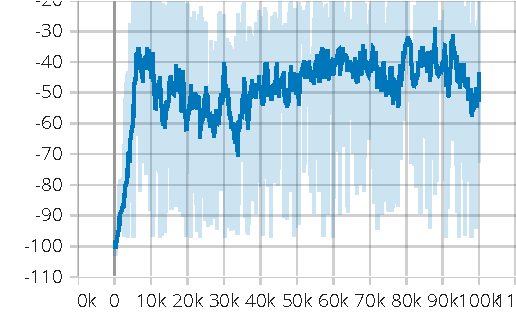
\includegraphics[width=\textwidth]{figures/cohesion-ctde.pdf}
            %\caption{Average cohesion factor}
            %\label{fig:cohesion-cc}
        \end{subfigure}
        \par\bigskip
        \begin{subfigure}[b]{0.32\textwidth}
            \centering
            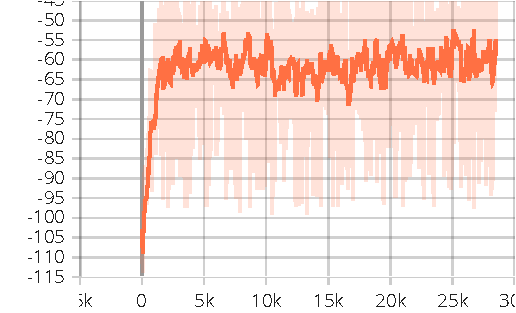
\includegraphics[width=\textwidth]{figures/reward-dtde.pdf}
            \caption{Total average reward}
            \label{fig:reward-dcc}
        \end{subfigure}
        \hfill
        \begin{subfigure}[b]{0.32\textwidth}
            \centering
            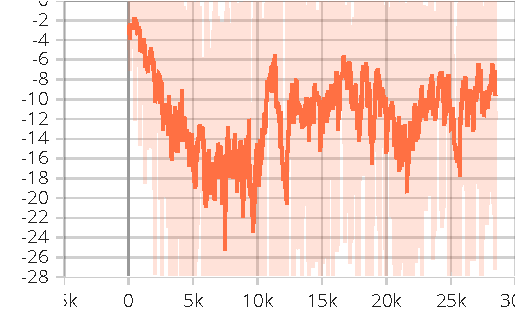
\includegraphics[width=\textwidth]{figures/collision-dtde.pdf}
            \caption{Average collision factor}
            \label{fig:collision-dcc}
        \end{subfigure}
        \hfill
        \begin{subfigure}[b]{0.32\textwidth}
            \centering
            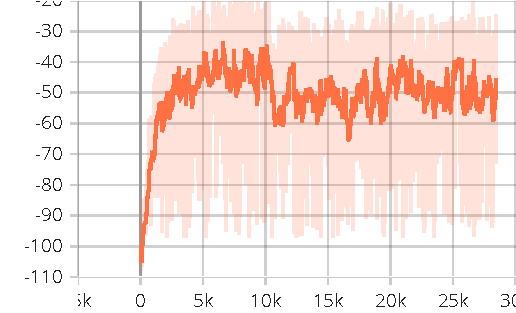
\includegraphics[width=\textwidth]{figures/cohesion-dtde.pdf}
            \caption{Average cohesion factor}
            \label{fig:cohesion-dcc}
        \end{subfigure}
    \caption{Cohesion and collision experiment results. The y-axis represents the reward value.
    The x-axis represents the total number of timesteps.
    The first three graphs show the results of the CDTE learning process, while the last three show the results of the DTDE learning process.}
    \label{fig:cc-results}
    \end{figure*}
    
    \begin{figure*}[t]
        \centering
        \begin{subfigure}[b]{0.25\textwidth}
            \centering
            \fbox{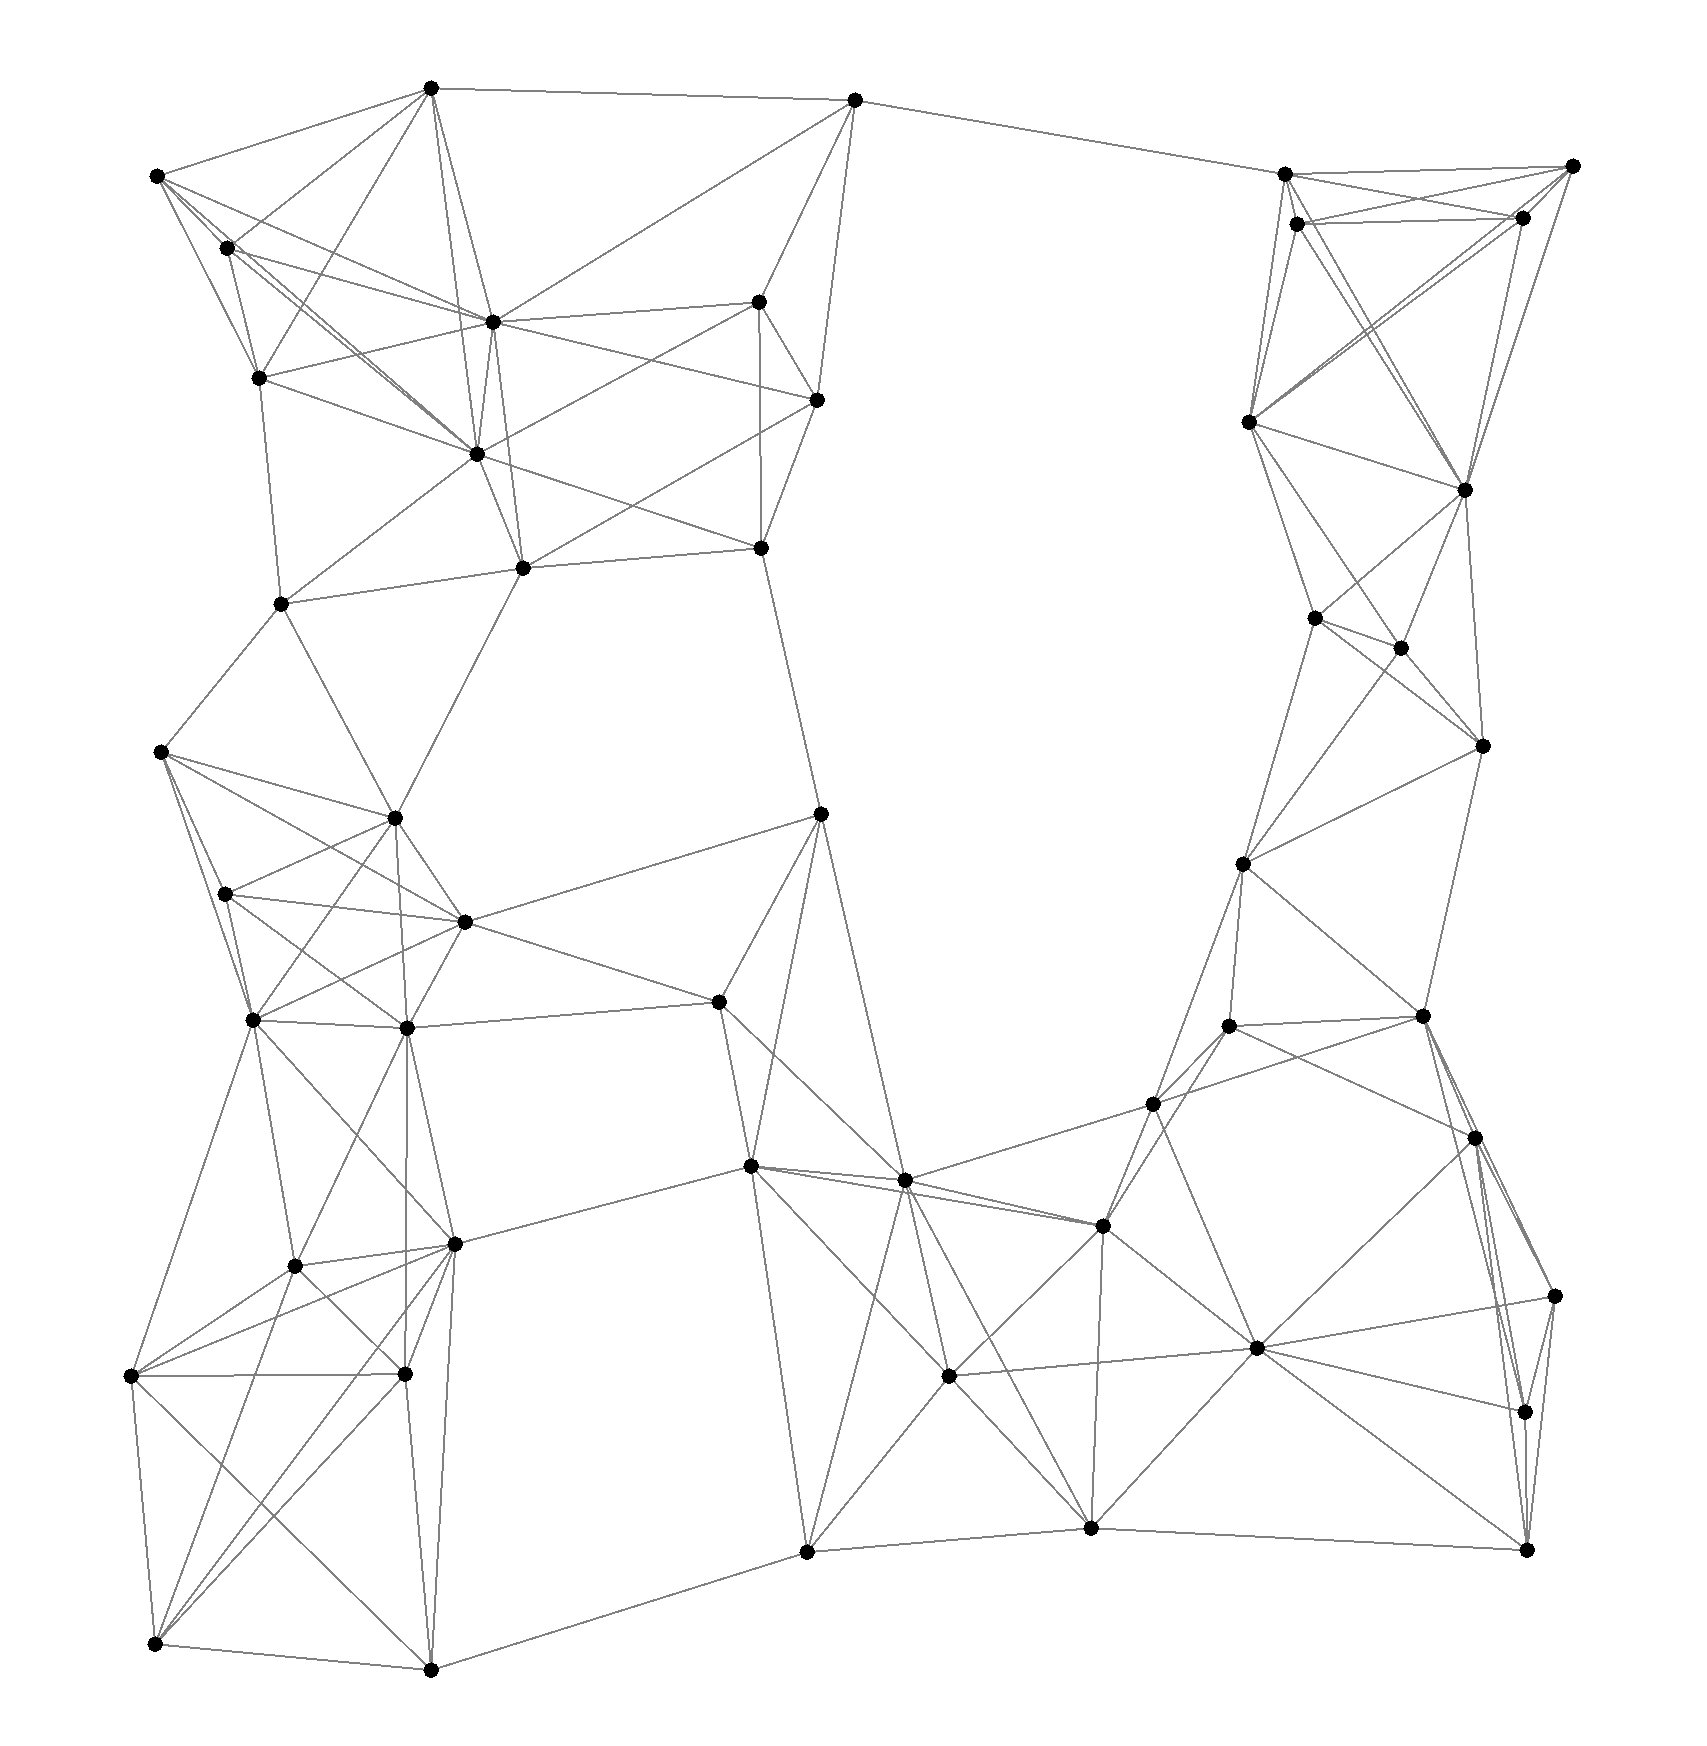
\includegraphics[width=\textwidth]{figures/1.png}}
            \caption{}
        \end{subfigure}
        \hfill
        \begin{subfigure}[b]{0.25\textwidth}
            \centering
            \fbox{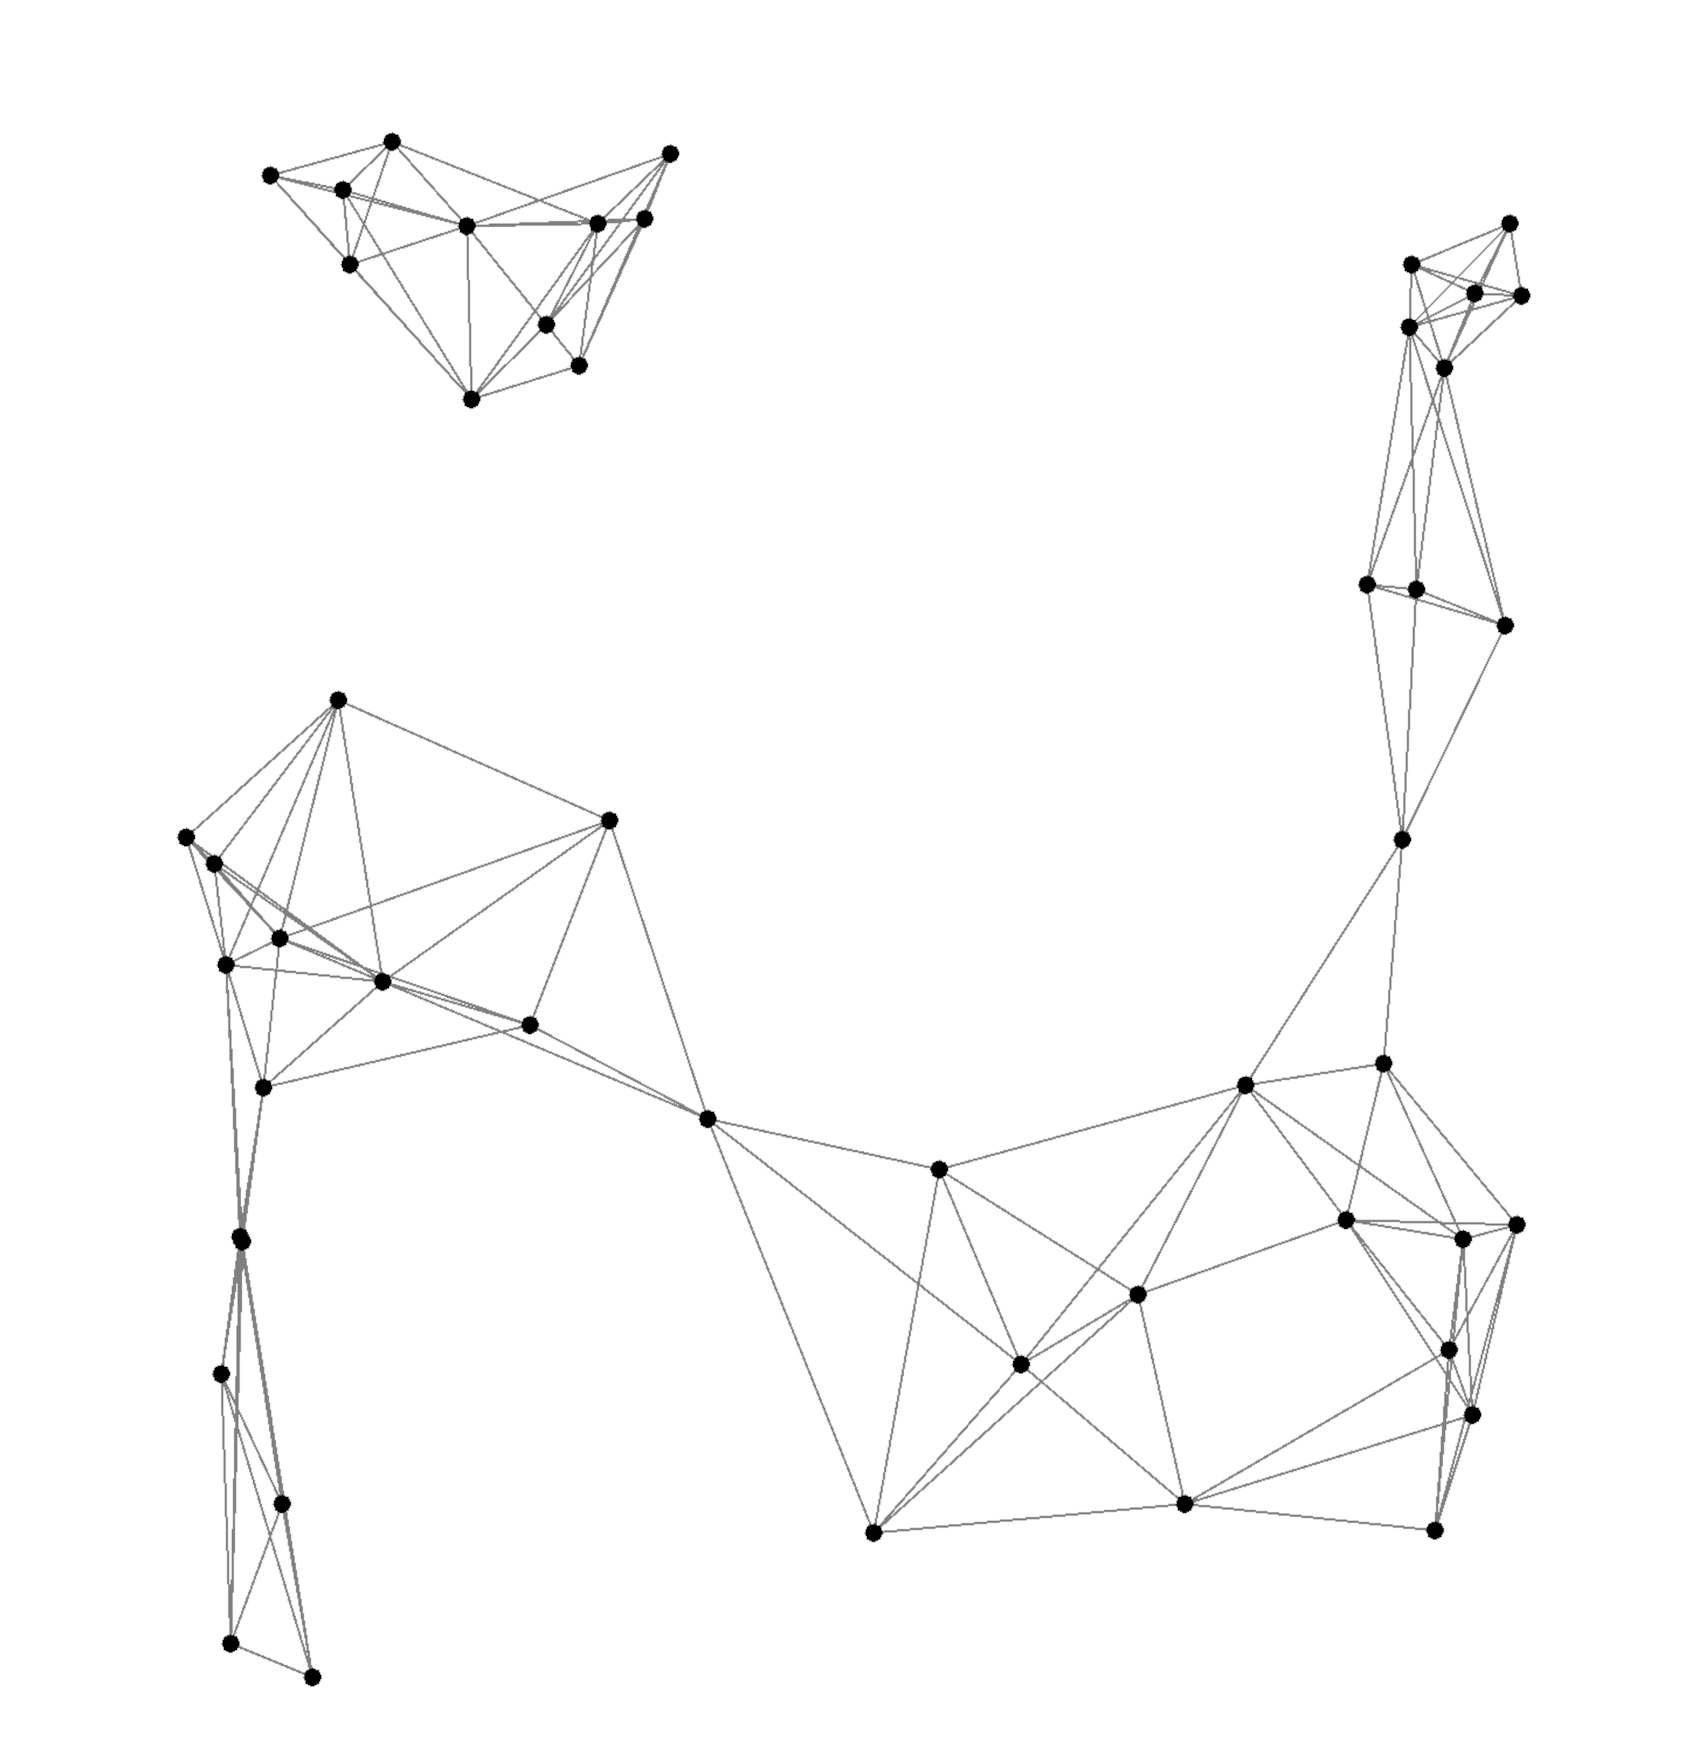
\includegraphics[width=\textwidth]{figures/4.png}}
            \caption{}
        \end{subfigure}
        \hfill
        \begin{subfigure}[b]{0.25\textwidth}
            \centering
            \fbox{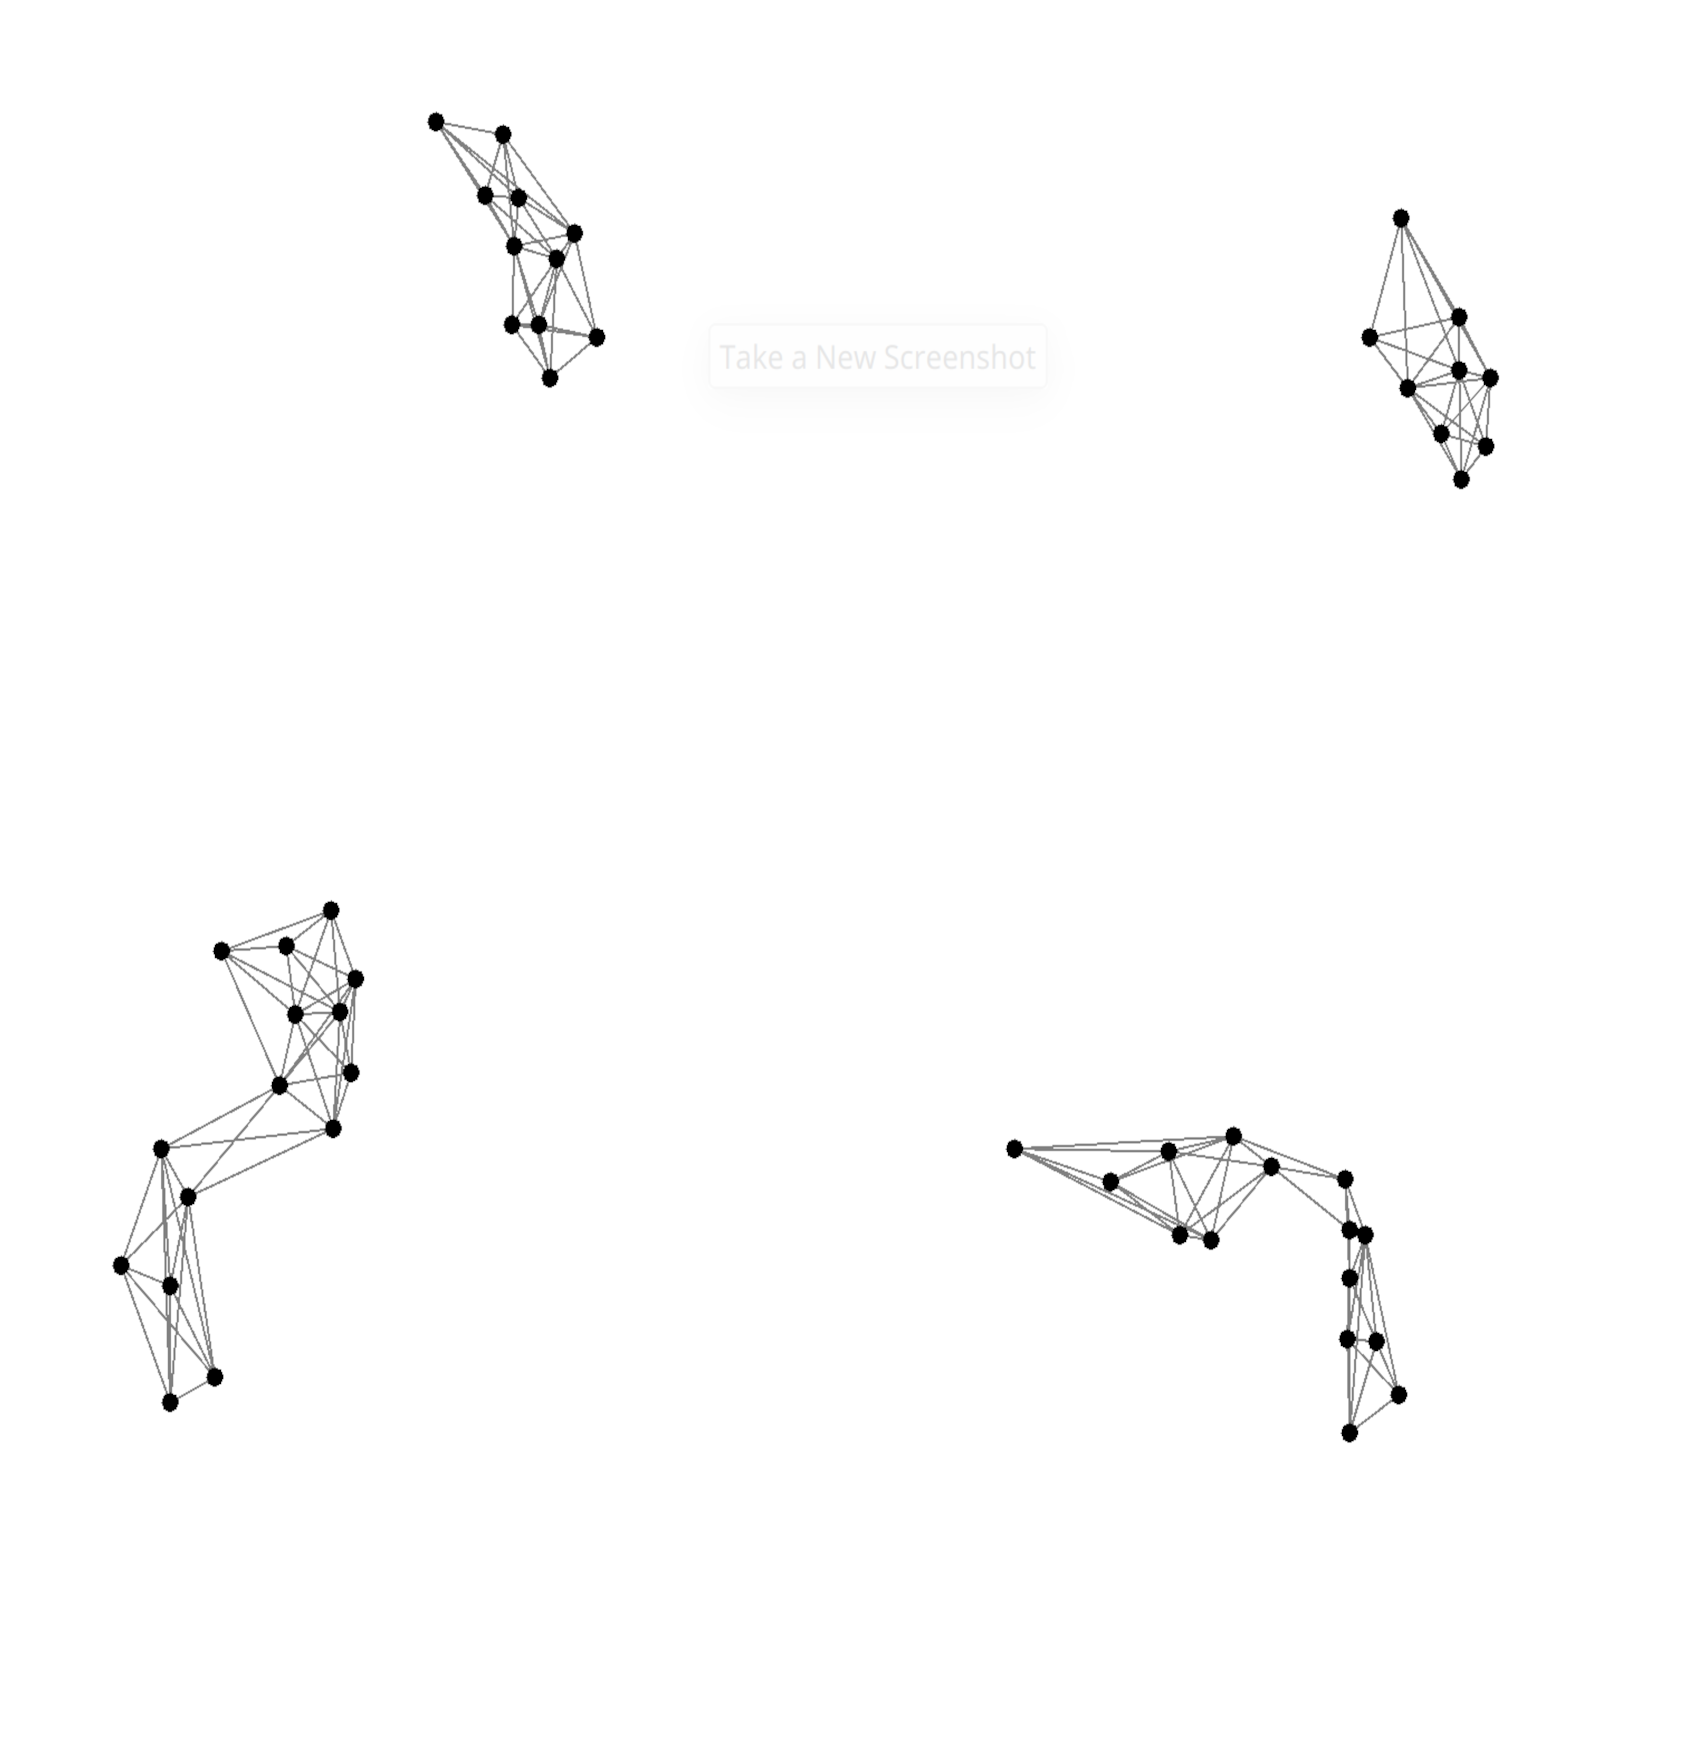
\includegraphics[width=\textwidth]{figures/7.png}}
            \caption{}
        \end{subfigure}
        \par
        \begin{subfigure}[b]{0.25\textwidth}
            \centering
            \fbox{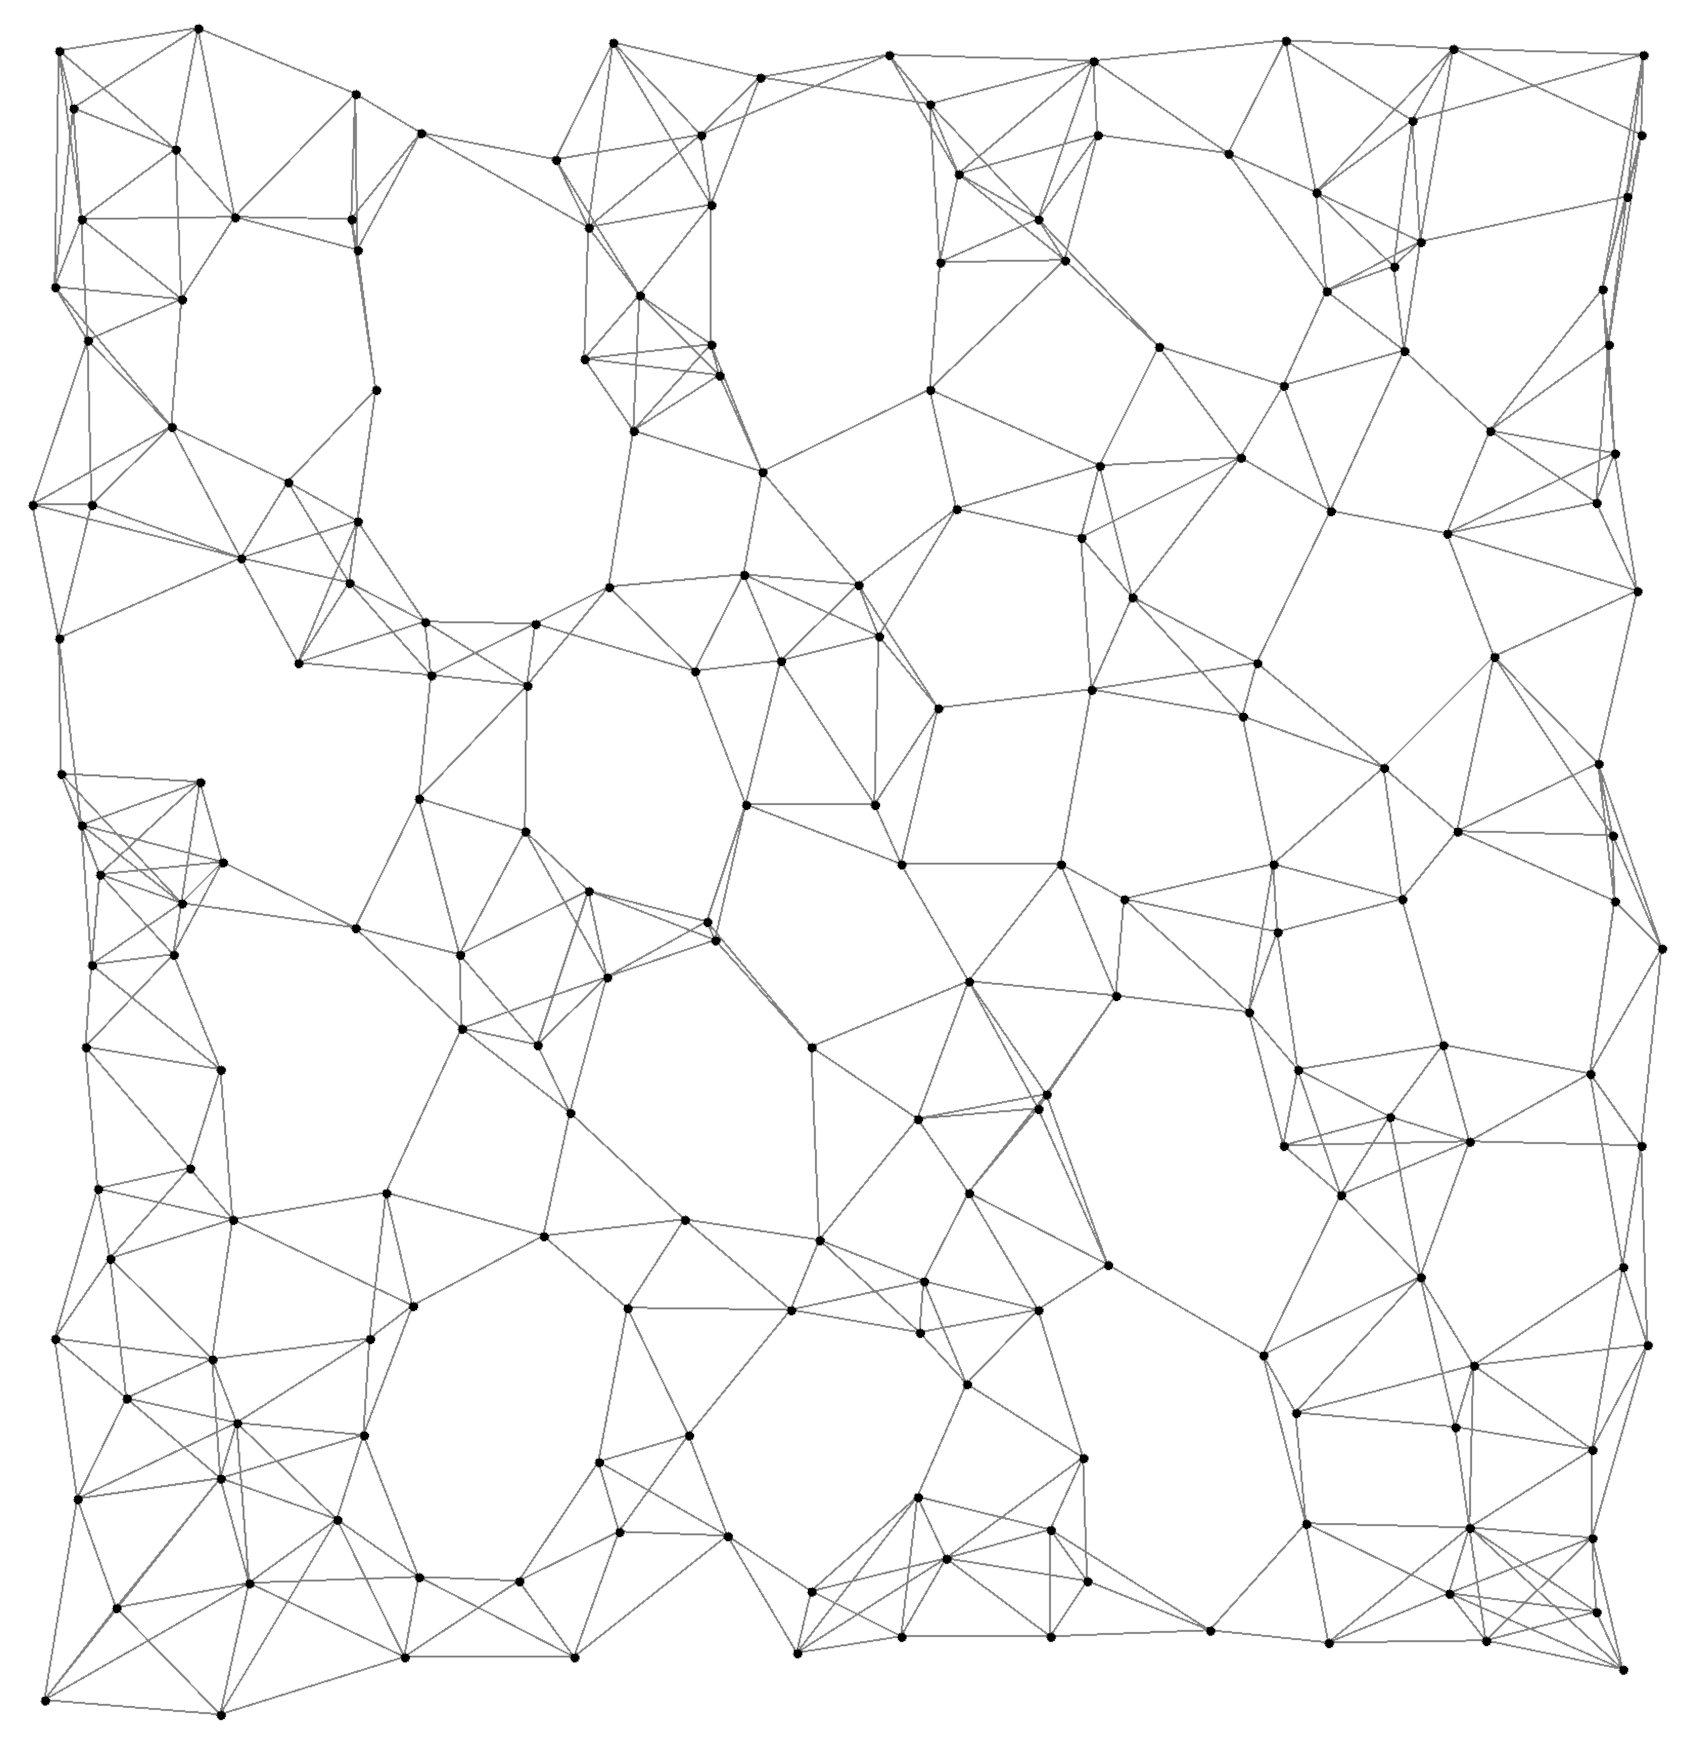
\includegraphics[width=\textwidth]{figures/1-large.png}}
            \caption{}
        \end{subfigure}
        \hfill
        \begin{subfigure}[b]{0.25\textwidth}
            \centering
            \fbox{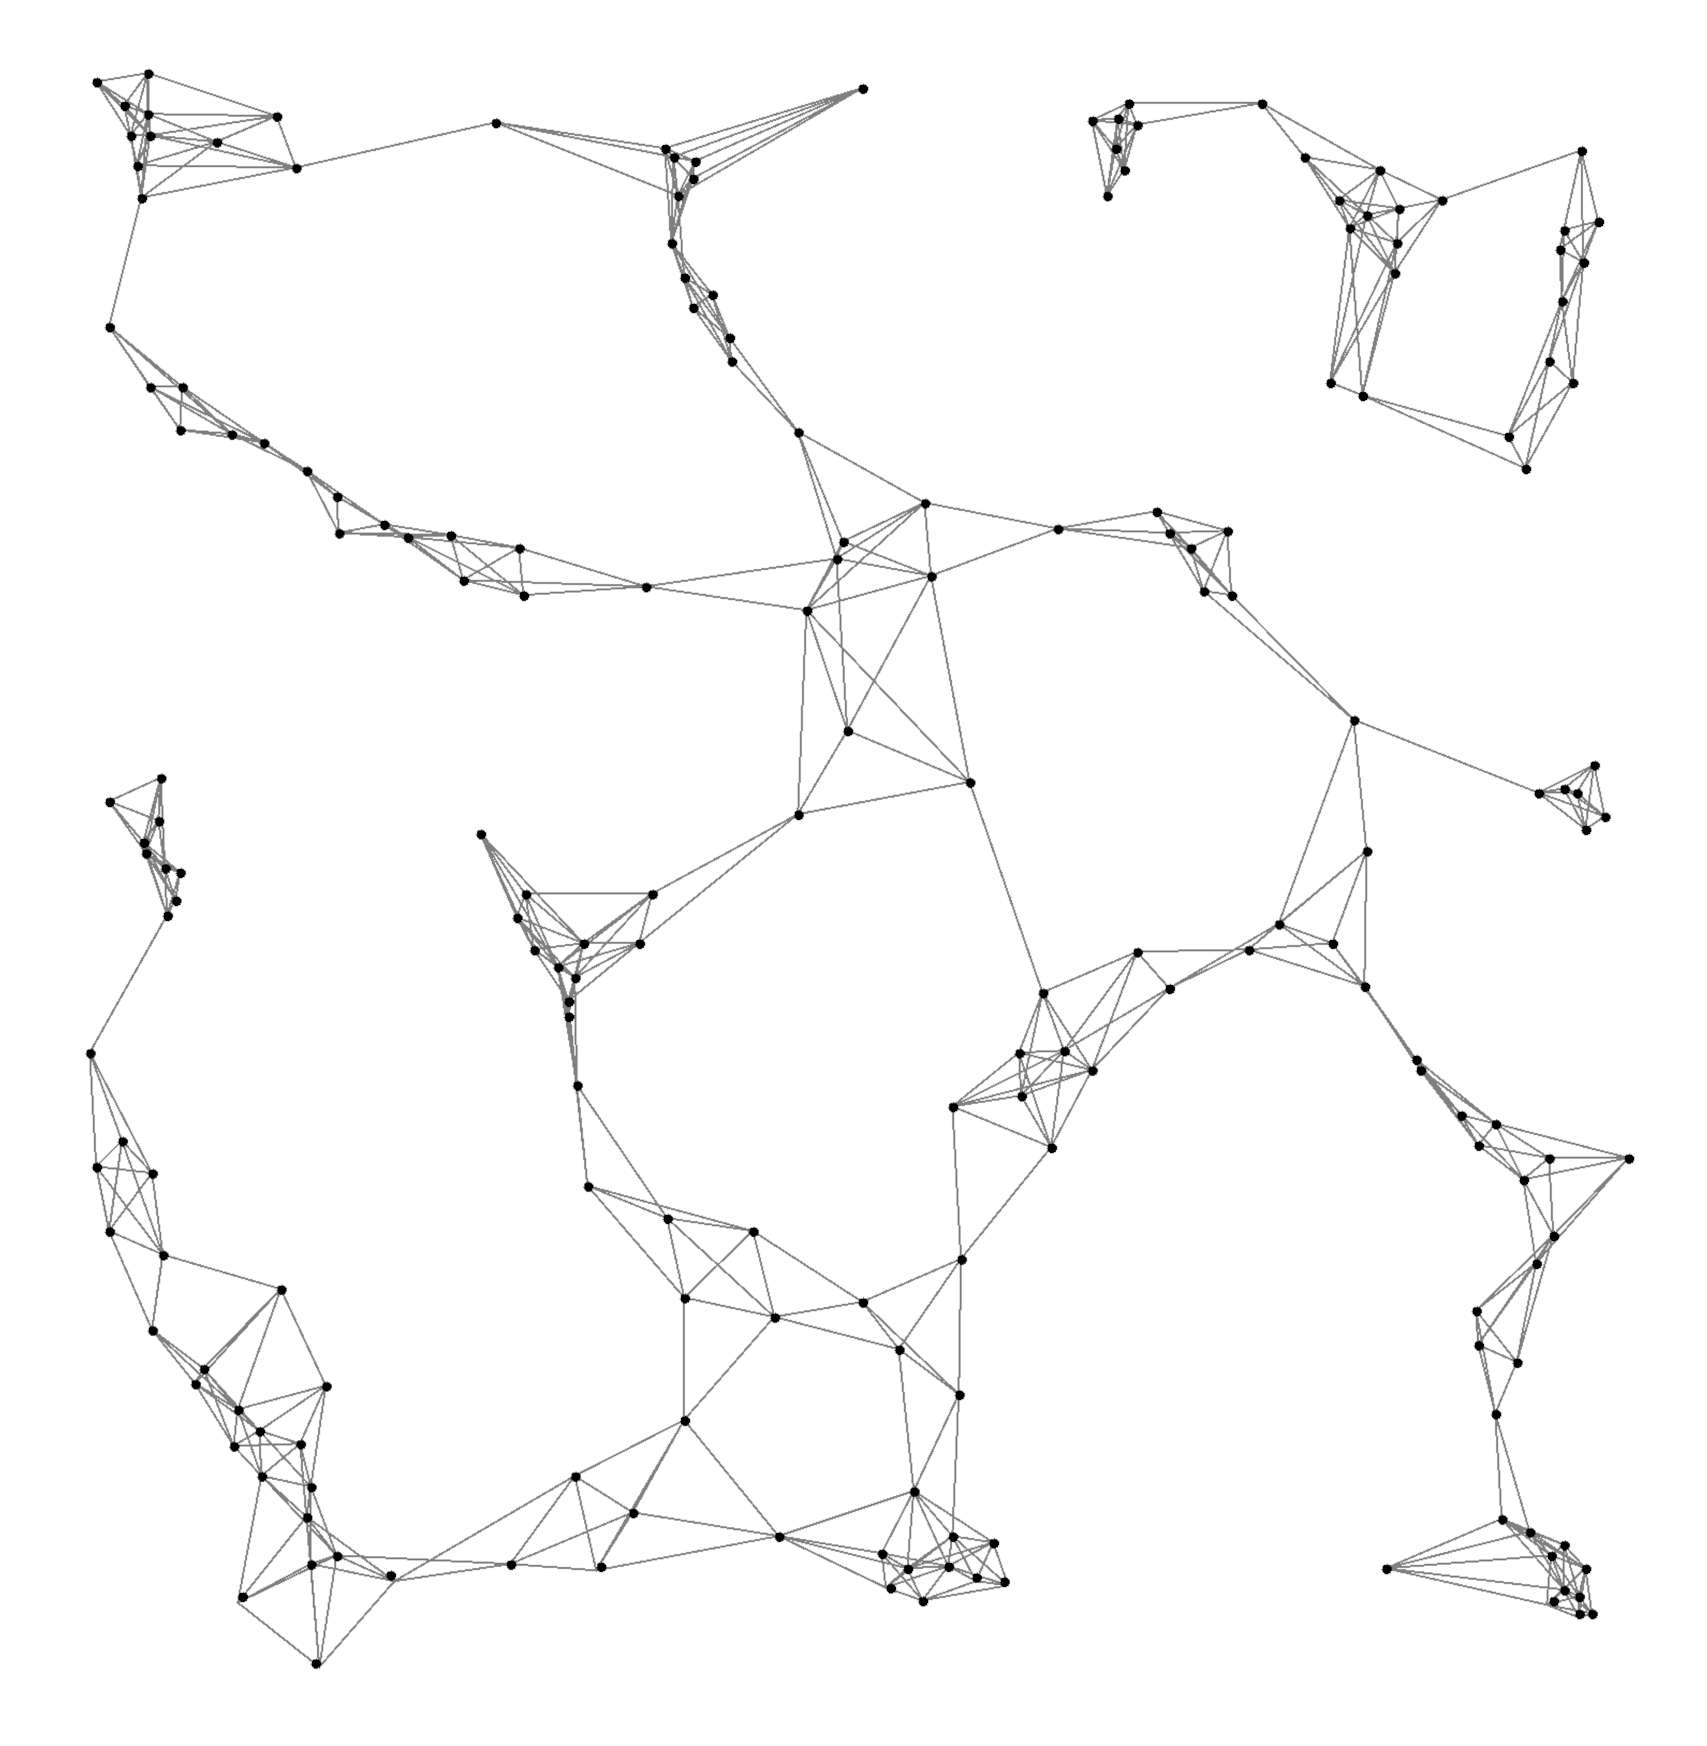
\includegraphics[width=\textwidth]{figures/3-large.png}}
            \caption{}
            \label{fig:sim2}
        \end{subfigure}
        \hfill
        \begin{subfigure}[b]{0.25\textwidth}
            \centering
            \fbox{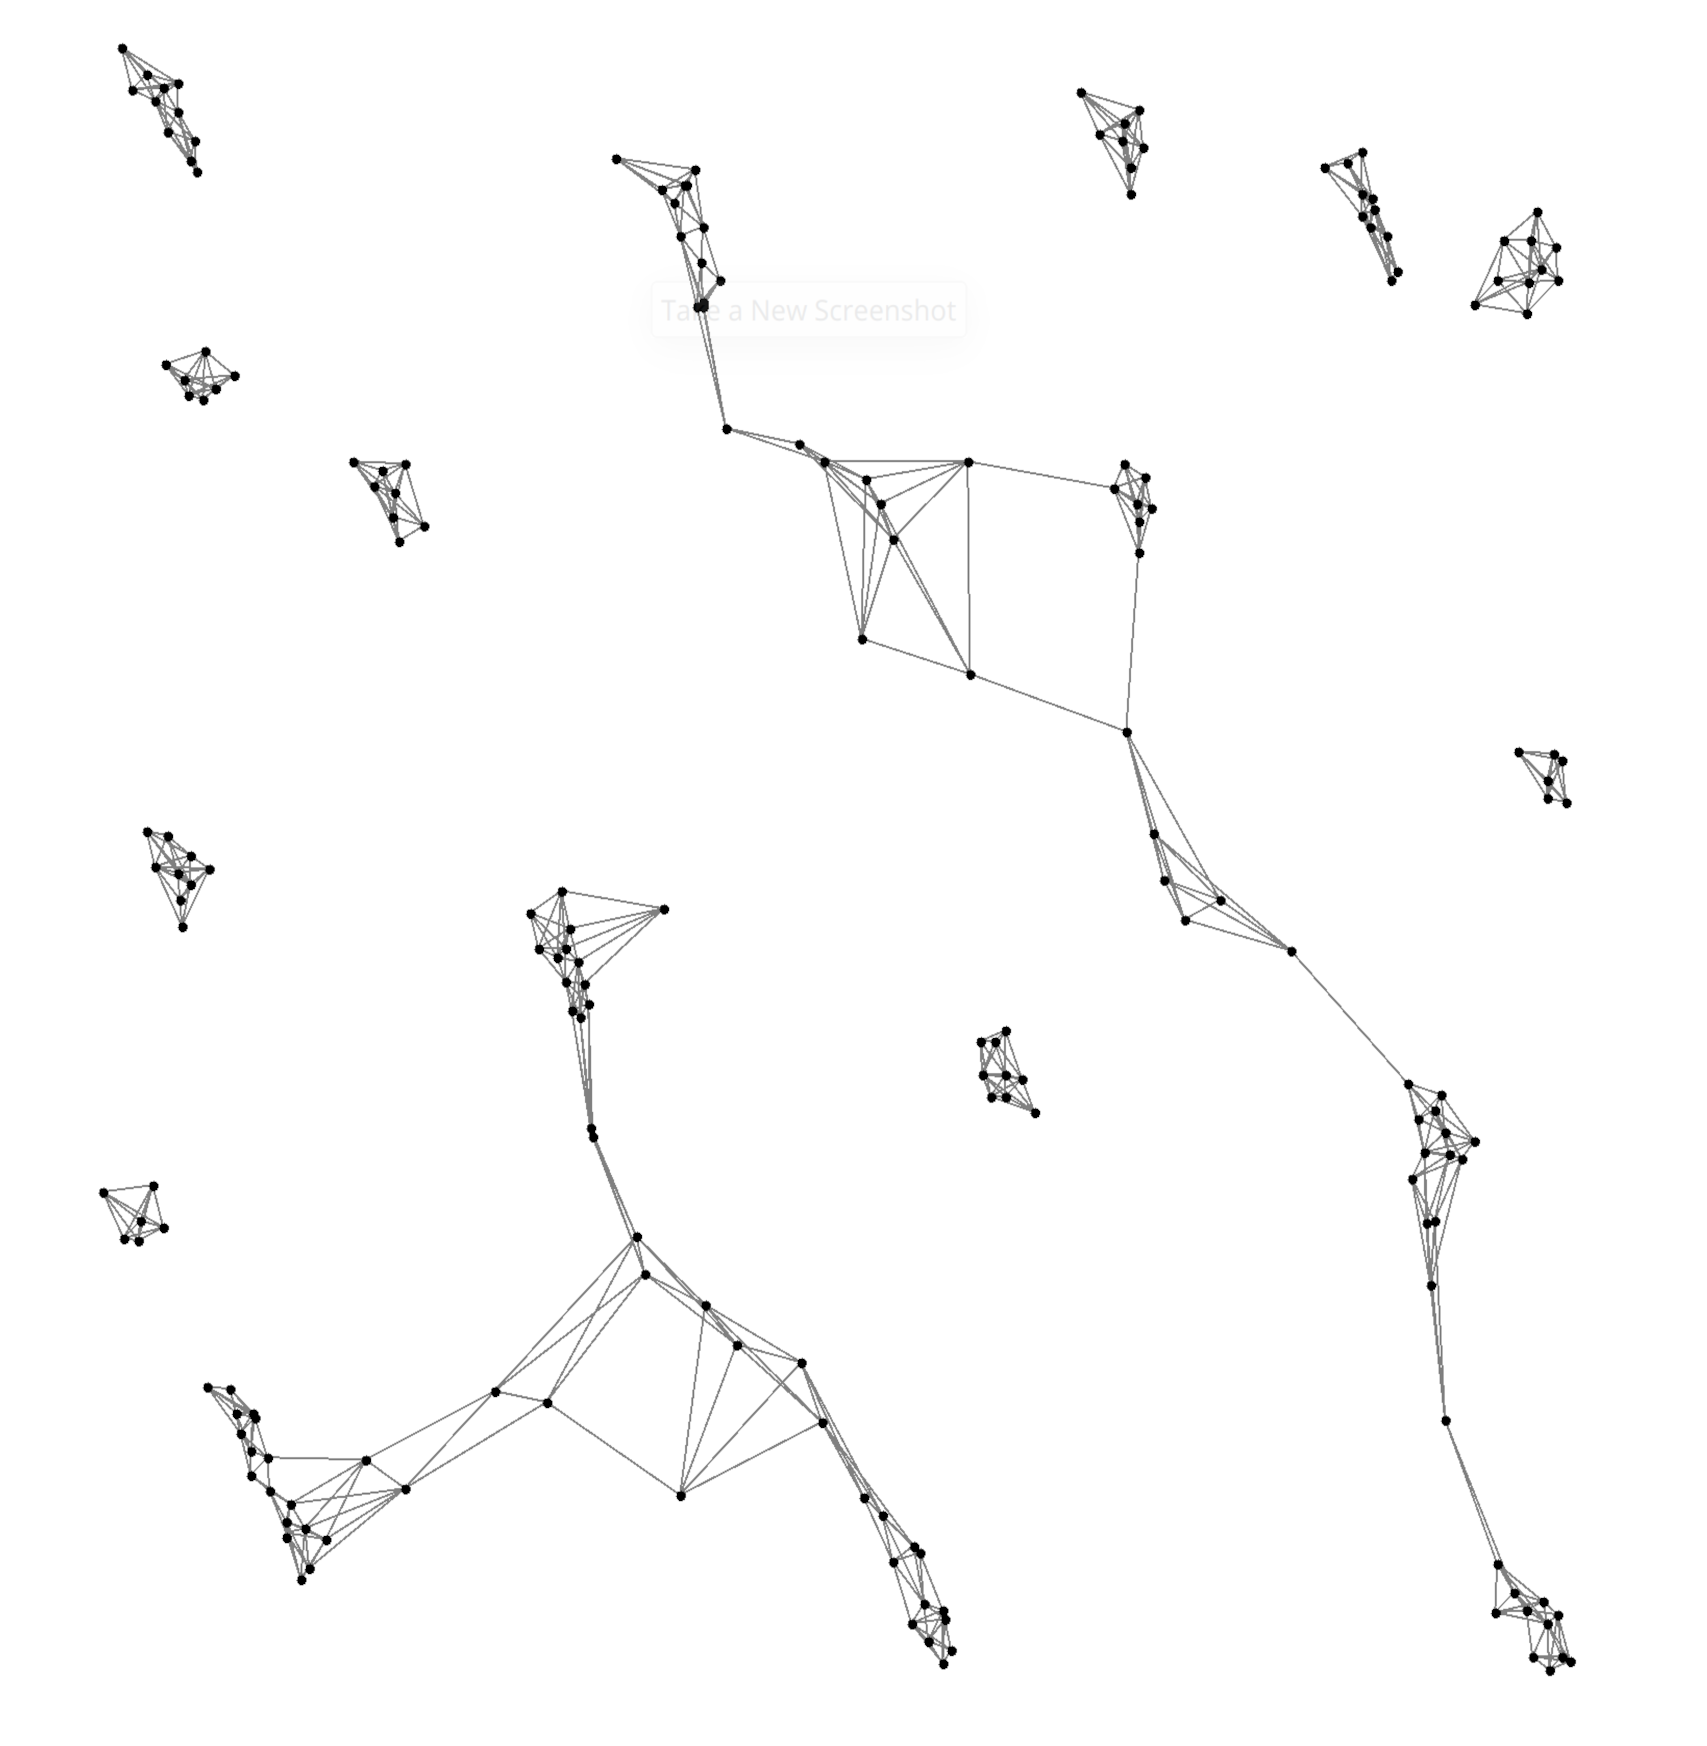
\includegraphics[width=\textwidth]{figures/4-large.png}}
            \caption{}
            \label{fig:sim3}
        \end{subfigure}
    \caption{Snapshots of the learned policy, the time flow is from left to right. 
    In the first row, there are 50 agents, whereas in the second row, there are 200 agents.
    In the last step of the simulation, the agents converged to a distance of approximately $\delta$.}
    \label{fig:simulation-snapshots}
    \end{figure*}
    
    \begin{figure*}[h!]
        \centering
        \begin{subfigure}[b]{0.32\textwidth}
            \centering
            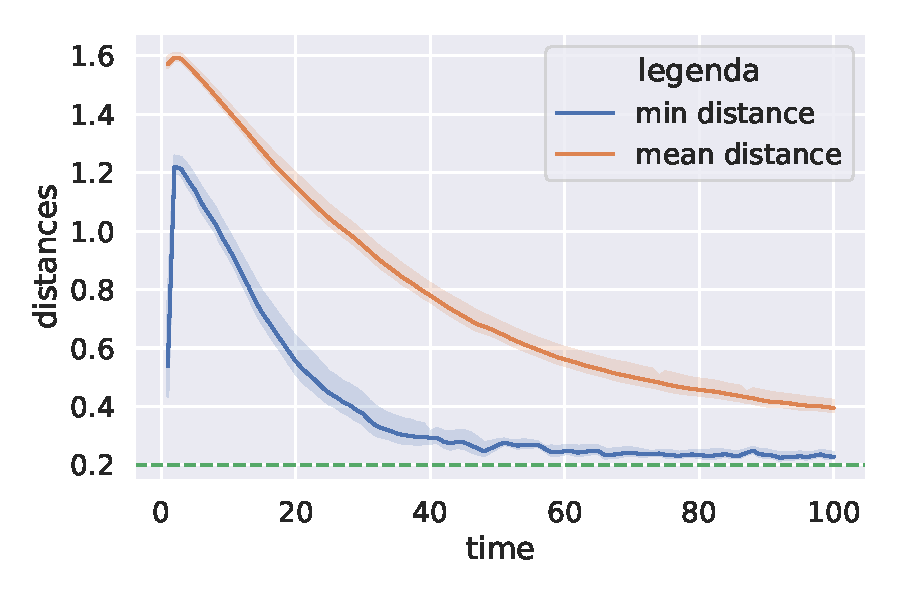
\includegraphics[width=\textwidth]{figures/data-50.pdf}
            \caption{50 agents}
        \end{subfigure}
        \hfill
        \begin{subfigure}[b]{0.32\textwidth}
            \centering
            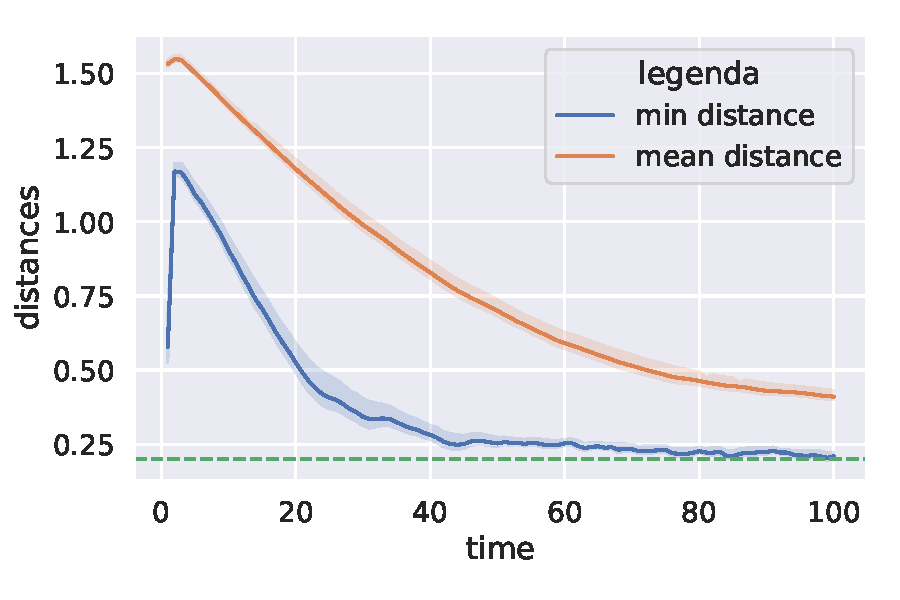
\includegraphics[width=\textwidth]{figures/data-100.pdf}
            \caption{100 agents}
        \end{subfigure}
        \hfill
        \begin{subfigure}[b]{0.32\textwidth}
            \centering
            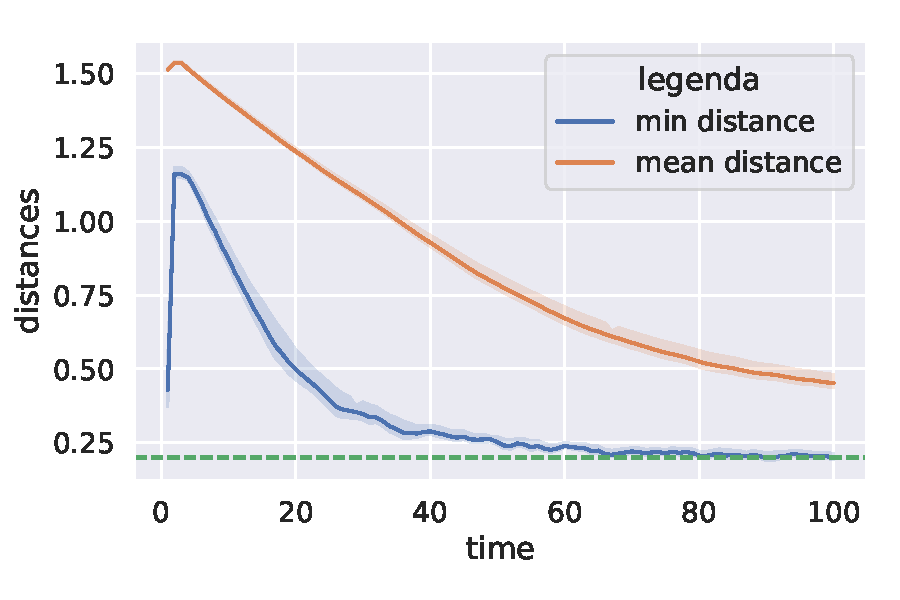
\includegraphics[width=\textwidth]{figures/data-200.pdf}
            \caption{200 agents}
        \end{subfigure}
    \caption{The performance of the learned policy. 
    The y-axis represents the distance between the agents.
    The x-axis represents the time.
    The green line is equal to $\delta$.
    In the charts, as the number of agents varies, the performance of the learned policy is similar.
    Moreover, the minimum (blue line) distance between the agents is always greater than $\delta$.
    The average distance (orange line) stays close to 2 * $\delta$ (after convergence).
    }
    \label{fig:test}
    \end{figure*}

\section{Follow the leader}

\paragraph{Description}
The aim of this experiment is to create a flock of drones with the task of avoiding \emph{collissions} while 
    following a special agent, the \emph{leader}. The goal is to learn a policy that guides each agent's movement
    based on the distances from neighbors and the leader. 

In our study, we examine an unbounded 2D environment where each agent has a set number of neighbours 
    (the five nearest, a hyper-parameter that is configurable), and can move in eight directions 
    (the four cardinal points and the four diagonals). During training the leader is placed in a random position and 
    cannot move, instead, during evaluation, the leader choose a random direction every $h$ time steps (a hyper-parameter that is configurable).

The \emph{reward function} is composed of two components. The first component is the \emph{collision factor},
    which is the same as the one used in the previous experiment, kicks in when the distance is less than 
    a given target distance $\delta$:
    \begin{equation}
        \label{eq:ftl-collision-factor-eq}
        \begin{split}
            \text{collision} = \begin{cases}
                0 & \text{if } d > \delta \\
                \exp\left(-\frac{d}{\delta}\right) & \text{otherwise}
            \end{cases}
        \end{split}
    \end{equation}
    The second component aims to reduce the distance between each agent and the leader:
    \begin{equation}
        \label{eq:ftl-distance-factor-eq}
        \text{distance to leader} = -d
    \end{equation}
    The overall reward function is defined as the sum of these two factors.

\paragraph{Results}
The experiment's training involved conducting $1000$ \emph{epochs}, each with $100$ \emph{episodes}, 
    using $50$ \emph{agents}, an \emph{environment} measuring $50$x$50$ metres and a \emph{target distance} $\delta$ set to $2$ metres.
    The training was conducted using a \emph{CTDE} process.

\Cref{fig:ftl-results} shows the results of the training. The graphs show that the learning algorithm optimizes one signal 
    at a time, with distance to leader tending towards zero and collision increasing. Nonetheless, after some epochs, 
    it is possible to see that the system had already found a balance between these two factors.

To verify the \emph{homogeneous policy} learned using the CTDE process, $16$ simulations were conducted, each with agents randomly
    positioned and varying the seeds. Given the homogeneous nature of the policy learned with CTDE, we also varied the 
    \emph{number of agents} by conducting simulations with $50$, $100$ and $200$ agents. According to our \emph{hypotheses}, this
    should not impact the \emph{quality} of the learned policy and its \emph{performance}. \Cref{fig:ftl-simulation-snapshots} shows 
    screenshots from a simulation with $50$ agents, illustrating how they gradually tend to get closer to the leader 
    (who is represented by the agent with the blue circle). \Cref{fig:test-ftl} shows the performance of the learned policy with $50$,
    $100$ and $200$ agents. From these graphs, it can be observed that the \emph{performance does not change significantly} with varying
    numbers of agents.

\begin{figure*}[t]
    \centering
    \begin{subfigure}[b]{0.9\textwidth}
        \centering
        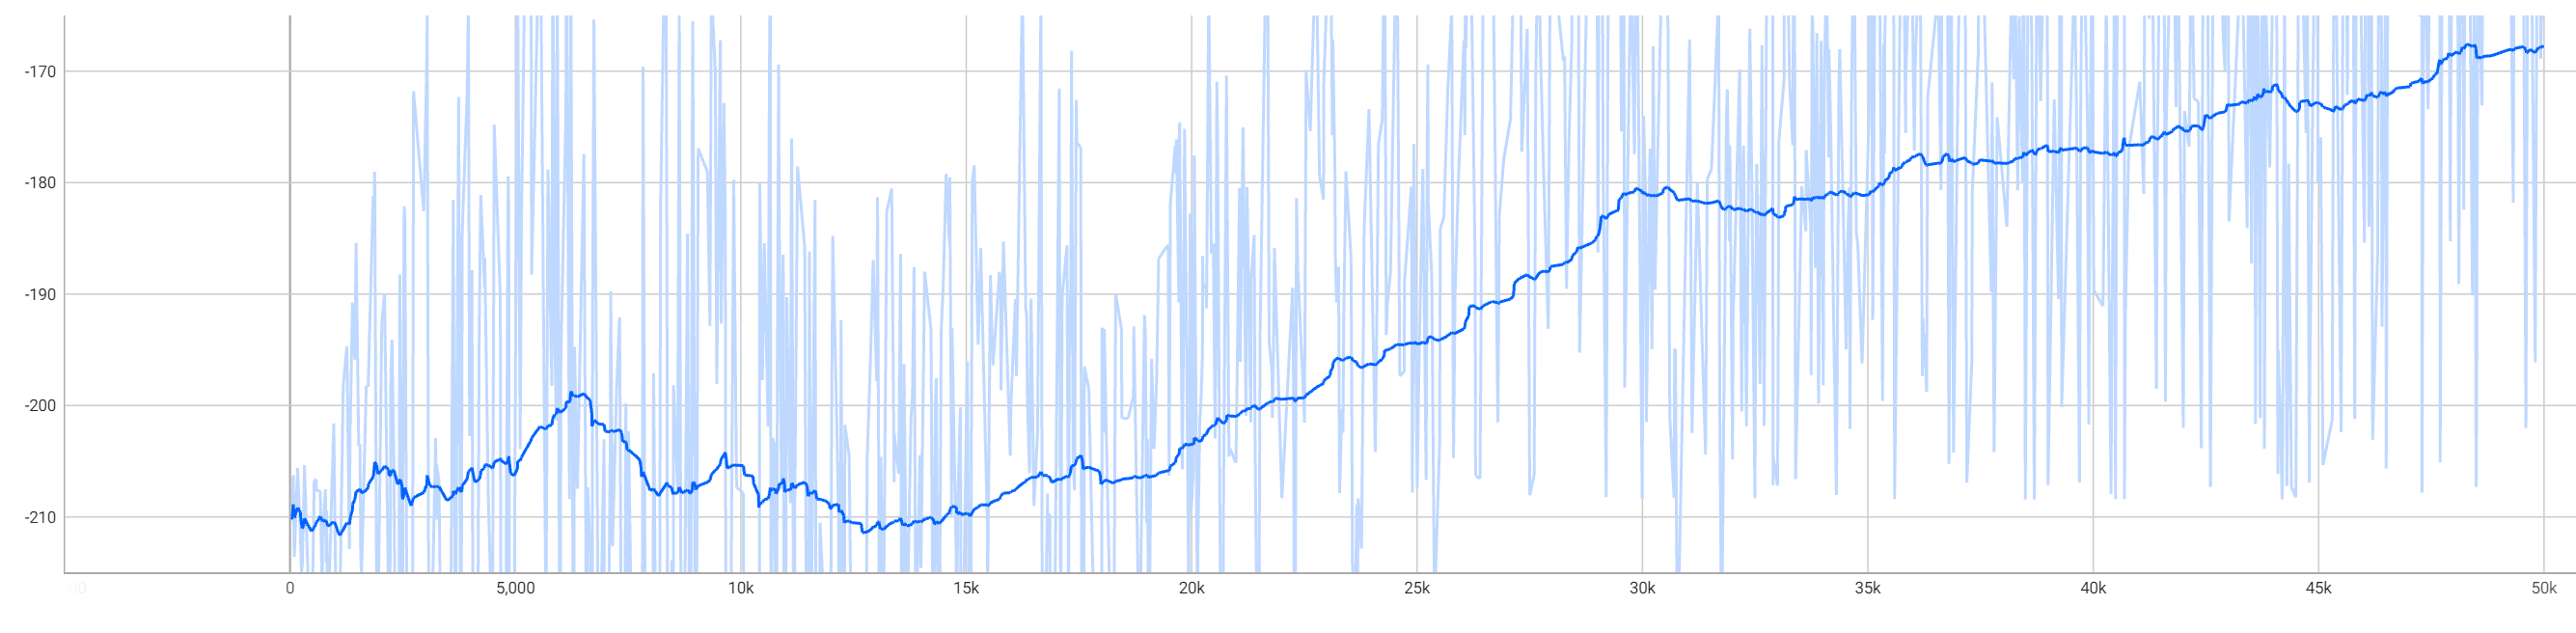
\includegraphics[width=\textwidth]{figures/ftl-reward.png}
        \caption{Total average reward}
    \end{subfigure}
    \hfill
    \begin{subfigure}[b]{0.9\textwidth}
        \centering
        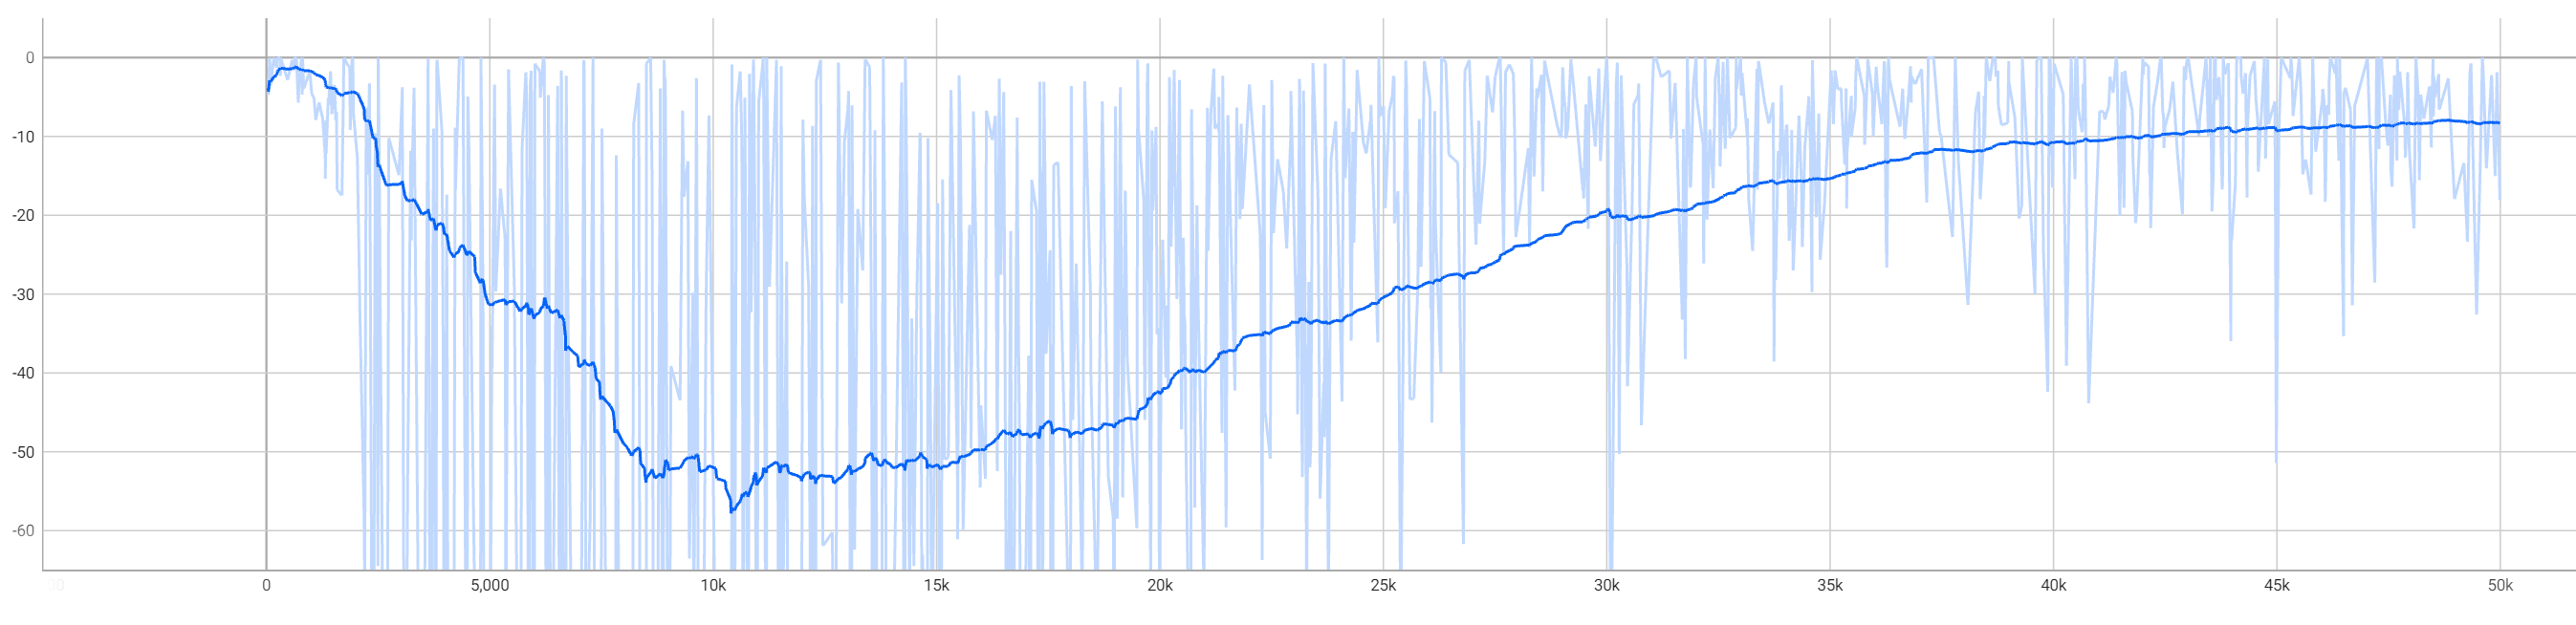
\includegraphics[width=\textwidth]{figures/ftl-collision.png}
        \caption{Average collision factor}
    \end{subfigure}
    \hfill
    \begin{subfigure}[b]{0.9\textwidth}
        \centering
        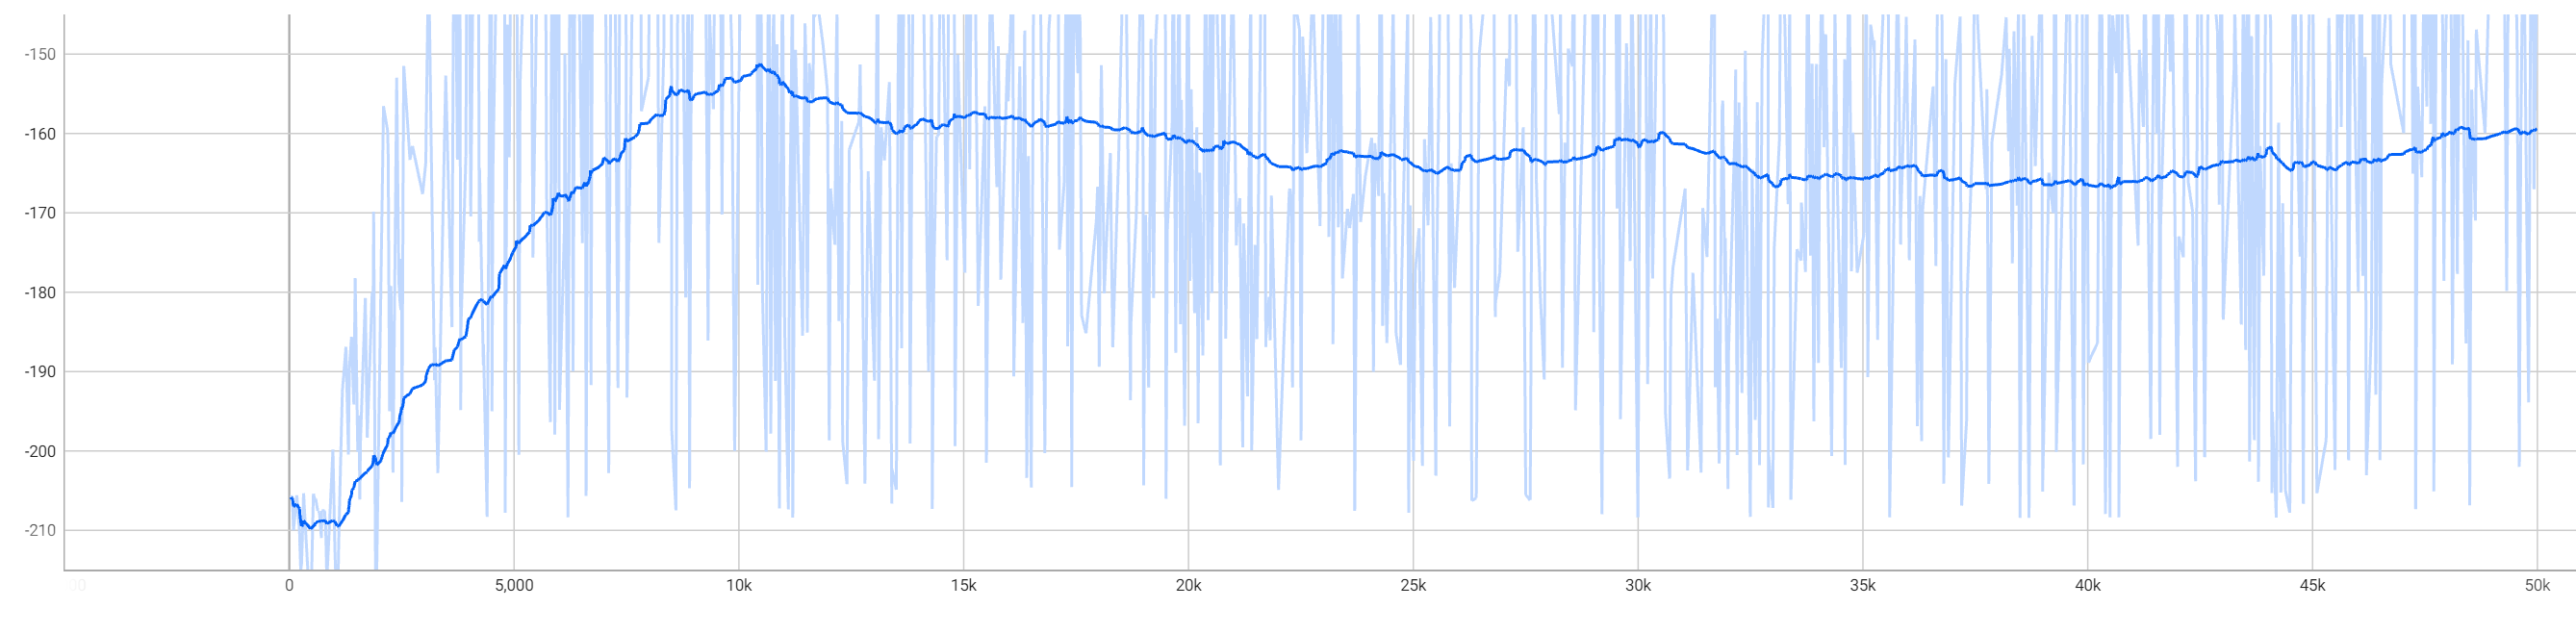
\includegraphics[width=\textwidth]{figures/ftl-distance-leader.png}
        \caption{Average distance to leader factor}
    \end{subfigure}
\caption{Follow the leader training experiment results. The y-axis represents the reward value.
The x-axis represents the total number of timesteps.}
\label{fig:ftl-results}
\end{figure*}

\begin{figure*}[t]
    \centering
    \begin{subfigure}[b]{0.25\textwidth}
        \centering
        \fbox{\includegraphics[width=\textwidth]{figures/ftl-start.png}}
        \caption{}
    \end{subfigure}
    \hfill
    \begin{subfigure}[b]{0.25\textwidth}
        \centering
        \fbox{\includegraphics[width=\textwidth]{figures/ftl-middle.png}}
        \caption{}
    \end{subfigure}
    \hfill
    \begin{subfigure}[b]{0.25\textwidth}
        \centering
        \fbox{\includegraphics[width=\textwidth]{figures/ftl-end.png}}
        \caption{}
    \end{subfigure}
\caption{Snapshots of the learned policy, the time flow is from left to right.}
\label{fig:ftl-simulation-snapshots}
\end{figure*}

\begin{figure*}[h!]
    \centering
    \begin{subfigure}[b]{0.32\textwidth}
        \centering
        \includegraphics[width=\textwidth]{figures/data-ftl-50.pdf}
        \caption{50 agents}
    \end{subfigure}
    \hfill
    \begin{subfigure}[b]{0.32\textwidth}
        \centering
        \includegraphics[width=\textwidth]{figures/data-ftl-100.pdf}
        \caption{100 agents}
    \end{subfigure}
    \hfill
    \begin{subfigure}[b]{0.32\textwidth}
        \centering
        \includegraphics[width=\textwidth]{figures/data-ftl-200.pdf}
        \caption{200 agents}
    \end{subfigure}
\caption{The performance of the learned policy. 
The y-axis represents the distance between the agents.
The x-axis represents the time.
The green line is equal to $\delta$.
In the charts, as the number of agents varies, the performance of the learned policy is similar.
The blue line represents the average distance between the agents, while the orange line represents
the average distance between each agent and the leader.
}
\label{fig:test-ftl}
\end{figure*}

\section{Framework limitations}
This section aims to highlight the main limitations present in the framework. These limitations are
 present for various reasons, some due to the nature of the domain, others due to implementation choices. 
 Furthermore, they provide a foundation for future improvements and expansion of the framework's capabilities.

\paragraph{Performance} 
Currently, a thorough and comprehensive performance benchmarking has not been carried out. This choice was made to 
    favor a simpler, more modular, and flexible design and implementation, following the principle of:
    ``Avoid premature optimization. First make it right, then make it fast" \cite{hyde2006fallacy}.
    Nonetheless, this aspect is crucial and will undoubtedly be considered in future work to ensure the tool is 
    fully prepared for community use.

\paragraph{Training and execution model} 
Currently, the framework offers solely two training and execution models, both among the most renowned in literature. 
    While these models can address various problems, they are not exclusive and may limit functionality in certain scenarios. 
    To facilitate user implementation and avoid the need to start from scratch, the framework must be expanded 
    to include additional models.

\paragraph{Scala-Python integration}
The integration between the framework, which is based on the Scala language, and PyTorch deep learning framework, 
    which is based on Python, is facilitated by the ScalaPy tool. However, despite the usefulness and potency of this tool, 
    it remains in an experimental and research phase that imposes certain usability and configuration restrictions, particularly 
    in non-Linux environments.

%----------------------------------------------------------------------------------------
\chapter{\conclusionsname}
\label{chap:conclusions}
%----------------------------------------------------------------------------------------
The work conducted in this thesis has resulted in the creation of \emph{ScaRLib}. The primary objective of this framework is to minimize complexity 
    in the design and building of \emph{multi-agent cyber-physical systems} (such as swarms of robots, IoT sensor networks, and various others) 
    exploiting and merging the potential of the two established methods employed in developing these systems, 
    namely: \emph{macro-programming} (i.e., aggregate computing) and \emph{artificial intelligence} (i.e., reinforcement learning).

In order to achieve this goal, the framework has been designed in a modular and extensible way, which has two main advantages.
    Firstly, users can effortlessly integrate fresh components including distinct simulators, various learning engines, and new learning algorithms or models.
    Secondly, users can leverage solely the elements of the framework that are required for their 
    specific project needs, without being duty-bound to use all of the modules.

A key aspect was to create abstractions within the reference domain to allow a concise and unambiguous definition of a new experiment. 
    Furthermore, standard training and execution models were pre-implemented (i.e., \emph{CTDE} and \emph{DTDE}), alongside a well-known learning algorithm (i,e., \emph{DQN}). 
    Afterwards, the core framework was combined with two tools, \emph{Alchemist} and \emph{ScaFi}. Alchemist permits the simulation of highly complex
    distributed systems whereas ScaFi enables the functional use of the aggregate computing paradigm through a Scala 
    programming language API. Additionally, a \emph{Domain Specific Language} was developed to declaratively specify 
    experiments and preemptively detect configuration errors during compile time, avoiding the need to wait for runtime occurrences.

In our opinion, the framework serves as an excellent point of initiation for developing such systems with a hybrid method 
    and streamlines the definition of complex new experiments. Our aim is to showcase the potential of this technique 
    and inspire the scientific community to delve further into this realm.

\section{Future work}

Despite the work that has been done, the reference domain is very broad, 
    and many aspects still require further improvement. This section aims to outline the primary areas 
    that need to be explored.

\paragraph{Performance}
The performance of the framework has only been assessed in relation to a small number of moderately 
    challenging use cases. However, it is essential to conduct further research in order to detect 
    potential bottlenecks and ensure that the minimum desired level of performance can be achieved, 
    thus meeting the diverse needs of users.

\paragraph{Execution model}
Currently, ScaRLib has pre-implemented integration with the Alchemist simulator via a basic, single execution model. 
    This model operates through each agent interacting with the environment at each timestep, followed by the
    environment awaiting action collection before transition to a new state. While this configuration is typical 
    in this field, it will be necessary to explore new solutions that enable the development of more specialised systems.


\paragraph{Learning framework}
The framework currently supports solely the PyTorch learning framework. However, it would be beneficial 
    to include additional frameworks, such as TensorFlow \cite{abadi2016tensorflow} or DL4J, to provide users with 
    a wider range of options.

\paragraph{Scala-Pyhton integration}
Currently, the framework utilises the ScalaPy tool to integrate Scala and Python programming languages. 
    Despite its potential, the tool has inherent research tool limitations, necessitating a judicious evaluation 
    of continuing its use or exploring alternative options, including custom bindings or third-party tools.

\paragraph{Online learning}
The inclusion of \emph{online learning} models in the framework, namely models that can continue learning after 
    deployment, would provide significant value. However, this is a field with few existing solutions, 
    made more complicated by the domain's multi-agent nature. We suggest leveraging 
    \emph{federated learning} \cite{zhang2021survey, abdulrahman2020survey} as an interesting approach, 
    enabling agents to exchange parts of their policy neural networks. 
    This approach may have the potential to \emph{distribute knowledge} within the system. 
    Nevertheless, additional research is required, and alternative options should also be taken into account.


%----------------------------------------------------------------------------------------
% BIBLIOGRAPHY
%----------------------------------------------------------------------------------------

%\nocite{*} % uncomment this to show all the reference in the .bib file
\bibliographystyle{plain}
\bibliography{bibliography}


\end{document}